%\RequirePackage{snapshot}

%\documentclass[letterpaper]{article}
\documentclass[a5paper]{article}

%% Language and font encodings
\usepackage[english]{babel}
\usepackage[utf8]{inputenc}
\usepackage[T1]{fontenc}

%% Sets page size and margins
%\usepackage[letterpaper,top=1in,bottom=1in,left=1in,right=1in,marginparwidth=1.75cm]{geometry}
\usepackage[a5paper,top=1cm,bottom=1cm,left=1cm,right=1.5cm,marginparwidth=1.75cm]{geometry}

%% Useful packages
\usepackage{amssymb, amsmath, amsthm} 
%\usepackage{graphicx}  %%this is currently enabled in the default document, so it is commented out here. 
\usepackage{calrsfs}
\usepackage{braket}
\usepackage{mathtools}
\usepackage{lipsum}
\usepackage{tikz}
\usetikzlibrary{cd}
\usepackage{verbatim}
%\usepackage{ntheorem}% for theorem-like environments
\usepackage{mdframed}%can make highlighted boxes of text
%Use case: https://tex.stackexchange.com/questions/46828/how-to-highlight-important-parts-with-a-gray-background
\usepackage{wrapfig}
\usepackage{centernot}
\usepackage{subcaption}%\begin{subfigure}{0.5\textwidth}
\usepackage{pgfplots}
\pgfplotsset{compat=1.13}
\usepackage[colorinlistoftodos]{todonotes}
\usepackage[colorlinks=true, allcolors=blue]{hyperref}
\usepackage{xfrac}					%to make slanted fractions \sfrac{numerator}{denominator}
\usepackage{enumitem}            
    %syntax: \begin{enumerate}[label=(\alph*)]
    %possible arguments: f \alph*, \Alph*, \arabic*, \roman* and \Roman*
\usetikzlibrary{arrows,shapes.geometric,fit}

\DeclareMathAlphabet{\pazocal}{OMS}{zplm}{m}{n}
%% Use \pazocal{letter} to typeset a letter in the other kind 
%%  of math calligraphic font. 

%% This puts the QED block at the end of each proof, the way I like it. 
\renewenvironment{proof}{{\bfseries Proof}}{\qed}
\makeatletter
\renewenvironment{proof}[1][\bfseries \proofname]{\par
  \pushQED{\qed}%
  \normalfont \topsep6\p@\@plus6\p@\relax
  \trivlist
  %\itemindent\normalparindent
  \item[\hskip\labelsep
        \scshape
    #1\@addpunct{}]\ignorespaces
}{%
  \popQED\endtrivlist\@endpefalse
}
\makeatother

%% This adds a \rewnewtheorem command, which enables me to override the settings for theorems contained in this document.
\makeatletter
\def\renewtheorem#1{%
  \expandafter\let\csname#1\endcsname\relax
  \expandafter\let\csname c@#1\endcsname\relax
  \gdef\renewtheorem@envname{#1}
  \renewtheorem@secpar
}
\def\renewtheorem@secpar{\@ifnextchar[{\renewtheorem@numberedlike}{\renewtheorem@nonumberedlike}}
\def\renewtheorem@numberedlike[#1]#2{\newtheorem{\renewtheorem@envname}[#1]{#2}}
\def\renewtheorem@nonumberedlike#1{  
\def\renewtheorem@caption{#1}
\edef\renewtheorem@nowithin{\noexpand\newtheorem{\renewtheorem@envname}{\renewtheorem@caption}}
\renewtheorem@thirdpar
}
\def\renewtheorem@thirdpar{\@ifnextchar[{\renewtheorem@within}{\renewtheorem@nowithin}}
\def\renewtheorem@within[#1]{\renewtheorem@nowithin[#1]}
\makeatother

%% This makes theorems and definitions with names show up in bold, the way I like it. 
\makeatletter
\def\th@plain{%
  \thm@notefont{}% same as heading font
  \itshape % body font
}
\def\th@definition{%
  \thm@notefont{}% same as heading font
  \normalfont % body font
}
\makeatother

%===============================================
%==============Shortcut Commands================
%===============================================
\newcommand{\ds}{\displaystyle}
\newcommand{\B}{\mathcal{B}}
\newcommand{\C}{\mathbb{C}}
\newcommand{\F}{\mathbb{F}}
\newcommand{\N}{\mathbb{N}}
\newcommand{\R}{\mathbb{R}}
\newcommand{\Q}{\mathbb{Q}}
\newcommand{\T}{\mathcal{T}}
\newcommand{\Z}{\mathbb{Z}}
\renewcommand\qedsymbol{$\blacksquare$}
\newcommand{\qedwhite}{\hfill\ensuremath{\square}}
\newcommand*\conj[1]{\overline{#1}}
\newcommand*\closure[1]{\overline{#1}}
\newcommand*\mean[1]{\overline{#1}}
%\newcommand{\inner}[1]{\left< #1 \right>}
\newcommand{\inner}[2]{\left< #1, #2 \right>}
\newcommand{\powerset}[1]{\pazocal{P}(#1)}
%% Use \pazocal{letter} to typeset a letter in the other kind 
%%  of math calligraphic font. 
\newcommand{\cardinality}[1]{\left| #1 \right|}
\newcommand{\domain}[1]{\mathcal{D}(#1)}
\newcommand{\image}{\text{Im}}
\newcommand{\inv}[1]{#1^{-1}}
\newcommand{\preimage}[2]{#1^{-1}\left(#2\right)}
\newcommand{\script}[1]{\mathcal{#1}}


\newenvironment{highlight}{\begin{mdframed}[backgroundcolor=gray!20]}{\end{mdframed}}

\DeclarePairedDelimiter\ceil{\lceil}{\rceil}
\DeclarePairedDelimiter\floor{\lfloor}{\rfloor}

%===============================================
%===============My Tikz Commands================
%===============================================
\newcommand{\drawsquiggle}[1]{\draw[shift={(#1,0)}] (.005,.05) -- (-.005,.02) -- (.005,-.02) -- (-.005,-.05);}
\newcommand{\drawpoint}[2]{\draw[*-*] (#1,0.01) node[below, shift={(0,-.2)}] {#2};}
\newcommand{\drawopoint}[2]{\draw[o-o] (#1,0.01) node[below, shift={(0,-.2)}] {#2};}
\newcommand{\drawlpoint}[2]{\draw (#1,0.02) -- (#1,-0.02) node[below] {#2};}
\newcommand{\drawlbrack}[2]{\draw (#1+.01,0.02) --(#1,0.02) -- (#1,-0.02) -- (#1+.01,-0.02) node[below, shift={(-.01,0)}] {#2};}
\newcommand{\drawrbrack}[2]{\draw (#1-.01,0.02) --(#1,0.02) -- (#1,-0.02) -- (#1-.01,-0.02) node[below, shift={(+.01,0)}] {#2};}

%***********************************************
%**************Start of Document****************
%***********************************************
 %find me at /home/trevor/texmf/tex/latex/tskpreamble_nothms.tex

%===============================================
%===============Theorem Styles==================
%===============================================

%================Default Style==================
%\theoremstyle{plain}% is the default. it sets the text in italic and adds extra space above and below the \newtheorems listed below it in the input. it is recommended for theorems, corollaries, lemmas, propositions, conjectures, criteria, and (possibly; depends on the subject area) algorithms.
%===============Highlight Style=================
\usepackage{xcolor}
\usepackage{mdframed}
%\newtheorem{mdtheorem}{Theorem}
\newenvironment{theorembold}%
  {\begin{mdframed}[backgroundcolor=gray!20]\begin{mdtheorem}}%
  {\end{mdtheorem}\end{mdframed}}
  
%==============Definition Style=================
\theoremstyle{definition}% adds extra space above and below, but sets the text in roman. it is recommended for definitions, conditions, problems, and examples; i've alse seen it used for exercises.
\newtheorem{theorem}{Theorem}
%\numberwithin{theorem}{section} %This sets the numbering system for theorems to number them down to the {argument} level. I have it set to number down to the {section} level right now.
\newtheorem*{theorem*}{Theorem} %Theorem with no numbering
\newtheorem{corollary}[theorem]{Corollary}
\newtheorem{conjecture}[theorem]{Conjecture}
\newtheorem{lemma}[theorem]{Lemma}
\newtheorem*{lemma*}{Lemma}
\newtheorem{proposition}[theorem]{Proposition}
\newtheorem*{proposition*}{Proposition}
\newtheorem{problemstatement}[theorem]{Problem Statement}

\newtheorem{definition}[theorem]{Definition}
\newtheorem*{definition*}{Definition}
\newtheorem{condition}[theorem]{Condition}
\newtheorem{problem}[theorem]{Problem}
\newtheorem{example}[theorem]{Example}
\newtheorem*{example*}{Example}
\newtheorem*{romantheorem*}{Theorem} %Theorem with no numbering
\newtheorem{exercise}{Exercise}
\numberwithin{exercise}{section}
\newtheorem{algorithm}[theorem]{Algorithm}

%================Remark Style===================
\theoremstyle{remark}% is set in roman, with no additional space above or below. it is recommended for remarks, notes, notation, claims, summaries, acknowledgments, cases, and conclusions.
\newtheorem{remark}[theorem]{Remark}
\newtheorem*{remark*}{Remark}
\newtheorem{notation}[theorem]{Notation}
%\newtheorem{claim}[theorem]{Claim}  %%use this if you ever want claims to be numbered
\newtheorem*{claim}{Claim}

%===============================================
%===========Document-specific commands==========
%===============================================
%\newcommand{\T}{\mathcal{T}}
%\newcommand{\B}{\mathcal{B}}
%\newcommand{\S}{\mathcal{S}}

%\newcommand{\arbcup}[1]{\bigcup\limits_{\alpha\in\Gamma}#1_\alpha}
%\newcommand{\arbcap}[1]{\bigcap\limits_{\alpha\in\Gamma}#1_\alpha}
%\newcommand{\arbcoll}[1]{\{#1_\alpha\}_{\alpha\in\Gamma}}
%\newcommand{\arbprod}[1]{\prod\limits_{\alpha\in\Gamma}#1_\alpha}
%\newcommand{\finitecoll}[1]{#1_1, \ldots, #1_n}
%\newcommand{\finitefuncts}[2]{#1(#2_1), \ldots, #1(#2_n)}


%================Start of document==============

\title{Topology - Fuller, 2017}
\author{Trevor Klar}

\begin{document}
\maketitle

\tableofcontents

\addcontentsline{toc}{section}{Introduction}
\section*{Introduction}

\begin{mdframed}[backgroundcolor=blue!20]
If you would like to copy and paste some of this \LaTeX \, for your own notes, you can download the .tex file \href{https://goo.gl/GYnmeX}{here}. (Warning, this file won't compile as-is, it needs a bunch of other files which are stored on my computer.)
\end{mdframed}

\begin{highlight}
Note: If you find any typos in these notes, please let me know at \\ \href{mailto:trevor.klar.834@my.csun.edu}{trevor.klar.834@my.csun.edu}. If you could include the page number, that would be helpful. 

Note to the reader: I have highlighted topics which seem important to me, but the emphasis is mine, not Professor Fuller's. Bear that in mind when studying. 
\end{highlight}

\subsection{Definitions}

\begin{definition*}
Two sets $A$ and $B$ have the \emph{same cardinality} if there exists a 1-1 and onto function $f:A \to B$. 

Then, we write $|A| = |B|$.
\end{definition*}

\begin{remark*} 
\begin{itemize}
\item if there exists a 1-1 function $f:A \to B$, we write $|A| \leq |B|$.
\item if there exists a 1-1 function $f:A \to B$, but no onto function exists, we write $|A| < |B|$.
\end{itemize}
\end{remark*}

\begin{definition*}
if $|A| = |\{1, \ldots , n\}|$, we say $A$ is \emph{finite}. (Assume $\emptyset$ is finite.)

If $A$ has a subset $S$ with $|S| = |\N|$, then $A$ is \emph{infinite}. (Equivalently, $A$ is infinite if it is not finite). 
\end{definition*}

\begin{definition*}
If $A$ is finite or $|A| = |\N|$, we say $A$ is \emph{countable}. Otherwise, $A$ is \emph{uncountable}.
\end{definition*}

\begin{proposition*}
$\Z$ and $\Q$ are countable. 
\end{proposition*}

\begin{remark*}
The argument for $\Q$ above (the standard zigzag pictorial chart) generalizes to show that a countable union of countable sets is countable. 
\end{remark*}

\begin{definition*}
Let $A$ be a set. The set of all subsets of $A$, denoted $\mathcal{P}(A)$ is called the \emph{power set} of $A$. (Remember, we always regard $\emptyset$ as a subset of $A$.)
\end{definition*}

\begin{example*}
$A = \{a,b\}$

$\mathcal{P}(A) = \{ \emptyset, \{a\}, \{b\}, \{a,b\} \}$.
\end{example*}

\begin{proposition*}
There is a 1-1 function $A \to \mathcal{P}(A)$.

proof: $a \to \{a\}$.
\end{proposition*}

\begin{theorem*}\textbf{(Cantor's Theorem)}

There is no onto function $a \to \mathcal{P}(A).$
\end{theorem*}

\begin{remark*}
Prop 0.2 and Thm 0.3 show that $|A| < |\powerset{A}|$.
\end{remark*}

\begin{theorem*}
$\R$ is uncountable.

\begin{proof}(sketch)
Show $(0,1)$ is uncountable. 

\begin{enumerate}
\item Let $\phi: (0,1) \to \powerset{\N}$ (This is uncountable by Cantor's thm)

\item Represent $x$ as a decimal in base 2, that is, $x=0.a_1a_2a_3...$ or 
$$x=\frac{a_1}{2}+\frac{a_2}{2^2}+\frac{a_3}{2^3}+\cdots \quad \text{where }a_i \in (0,1).$$ 

\item Now, define $\phi(x) = \{n:a_n=1\}$. So, $\phi$ returns a list of the base-2 decimal places which contain a 1, when representing $x$ as a base-2 decimal.

\item This almost works, but it is not well-defined.

\item Note that if $x=0.[\text{zeros and ones}]1$, then $x=0.[\text{zeros and ones}]01111\ldots$. So, this reresentation is not unique, so our function isn't technically well-defined. 

\item To get a well-defined function, we must make the convention that if $x=0.[\text{zeros and ones}]1$, we define $\phi(x)$ according to that representation, not the repeating version. 

\item With this convention, we have a $\phi: (0,1) \to \powerset{\N}$ which is 1-1, but not onto. However, it is onto $\powerset{\N}-T$, where $T$ is the set of all subsets of $\N$ containing $\{N, N+1, N+2, \ldots, \}$ for some $N$. 

\item Now, $T$ is a countable set, so $\powerset{\N}-T$ is still uncountable, so we don't have a problem. 
\end{enumerate}
\end{proof}
\end{theorem*}

\begin{definition*}
Let $f:X \to Y$, $B \subset	 Y$. The \emph{preimage} of $B$ under $f$ is $f^{-1}(B)=\{x:f(x)\in B\}$.

We often write $f^{-1}(\{y\})=f^{-1}(y)$, to suppress notation. This could evaluate to a singleton, or to a set of multiple points. 
\end{definition*}

\subsection{Motivation}

\begin{definition*}
$\R^n=\{x_1,\ldots x_n\}$

$d(\vec{x}, \vec{y})=\sqrt{\sum(x_i-y_i)^2}$
\end{definition*}

\begin{definition*}(n=1)

$f:\R \to \R$ is \emph{continuous} at $x_0$ if for every $\epsilon > 0$ there is a $\delta > 0$ such that $|x-x_0| < \delta \implies |f(x)-f(x_0)| < \epsilon$.
\end{definition*}

\begin{definition*}
In $\R^n$, $B(x_0, r)=\{x\in \R^n : d(x,x_0) < r\}$. We call this an \emph{open ball} with center $x_o$ and radius $r$. 
\end{definition*}

\begin{definition*}(general n)

$f:\R^n \to \R^m$ is continuous at $\vec{x_0}$ if for every $\epsilon > 0$ there is a $\delta > 0$ such that $d(\vec{x},\vec{x_0}) < \delta \implies d(\vec{f(x)},\vec{f(x_0)}) < \epsilon$.

or, $\vec{x} \in B(\vec{x_0},\delta) \implies \vec{f(x)} \in B(\vec{f(x_0)},\epsilon)$

or, $\vec{x} \in B(\vec{x_0},\delta) \implies \vec{x} \in f^{-1}(B(\vec{f(x_0)},\epsilon))$

or, $B(\vec{x_0},\delta) \subset f^{-1}(B(\vec{f(x_0)},\epsilon))$
\end{definition*}

\begin{definition*}
A set $U \subset \R^n$ is \emph{open} if for all $x \in U$, there is a real number $r(x)>0$ such that $B(x,r(x))\subset U$. (The set contains a neighborhood of every element in the set)
\end{definition*}

\noindent \textbf{Facts about open sets:}
\begin{enumerate}
\item Open balls are open sets. 
\begin{proof}
Let $x \in B(x_0,R)$. Let $r(x)=R-d(x,x_0)$. Let $x' \in B(x,r(x))$. 

Now, $d(x',x_0) \leq d(x',x) + d(x,x_0)$

$\quad < R-d(x,x_0) + d(x,x_0)$

$\quad = R$

So, $x' \in B(x_0,R)$, and $B(x,r(x)) \subset B(x_0,R)$.
\end{proof}
\item Every open set $U$ in $\R^n $ is a union of open balls. 
\item $\R^n$ and $\emptyset$ are open. 
\item Arbitrary unions of open sets are open. That is, suppose $\{U_\alpha\}_{\alpha \in \Gamma}$ is a collection of open sets. Then, $\bigcup_{\alpha \in \Gamma} U_\alpha$ is open. 
\item If $U_1, U_2$ are open, then $U_1 \cap U_2$ is open. This also works with any finite number of sets. 
\end{enumerate}

\begin{theorem*}
Given $f:\R^n \to \R^m$\\
The following are equivalent:
\begin{enumerate}
\item $f$ is continuous at $x$ for all $x \in \R^n$ (with $\epsilon$-$\delta$ definition).
\item $f^{-1}(V)$ is open for all open $V \in \R^n$. 
\begin{proof}\mbox{}\\
Show that statement (1) $\implies$ (2). \\
Let $x \in f{-1}(V)$. Then $f(x) \in V$. Since $V$ is open, there exists some $\epsilon > 0$ such that $B(f(x),\epsilon)\subset V$. Since $f$ is contionuous at $x$, there is a $\delta >0$ such that 
$$B(x,\delta)\subset f^{-1}(B(f(x),\epsilon)) \subset	f^{-1}(V).$$ 

Show that statement (2) $\implies$ (1).\\
Let $x \in \R^n$, and let $\epsilon >0$. Since $B(f(x),\epsilon)$ is open, by assumption $f^{-1}(B(f(x),\epsilon))$ is open in $\R^n$. Note that $x \in f^{-1}(B(f(x),\epsilon))$. So, there exists some $\delta >0$ such that $B(x,\delta) \subset f^{-1}(B(f(x),\epsilon))$. So, $f$ is continuous at $x$. 
\end{proof}
\end{enumerate}
\end{theorem*}

All that is meant to motivate what follows:

\section{Topologies}

\subsection{Definition and examples of a topology}

\begin{highlight}
\begin{definition*}
Let $X$ be a set. A collection $\pazocal{T}$ of subsets of $X$ is a \emph{topology on $x$} if:
\begin{enumerate}
\item $\emptyset \in \T, X \in \T$
\item If $U_\alpha \in \T$ for all $\alpha \in \Gamma$, then 
$$\bigcup_{\alpha \in \Gamma}U_\alpha \in \T.$$
($\T$ is closed under arbitrary unions)
\item If $U_1 \in \T$ and $U_2 \in \T$, then $U_1\cap U_2 \in \T$. \\
($\T$ is closed under finite intersections)
\end{enumerate}
\end{definition*}
\end{highlight}

\begin{definition*}
The sets in $\T$ are called \emph{open sets}. 
\end{definition*}

\begin{definition*}
We will refer to $X$ together with a topology $\T$ on $X$ as a \emph{topological space} (or simply a \emph{space}, when context is clear).
\end{definition*}

\begin{definition*}
We will sometimes denote a topological space as $(X, \T)$.
\end{definition*}

\begin{highlight}
\begin{definition*}
A function $f:(X, \T_x) \to (Y, \T_y)$ is \emph{continuous} if $\preimage{f}{V}\in\T_x$ for all $V \in \T_y$.\\
(That is, iff the preimage of an open set is open)
\end{definition*}
\end{highlight}

\begin{remark*}
A set $V \in \T$ means that the set $V$ is open under the rules for $\T$ which define open sets. 
\end{remark*}

\begin{example*}\textbf{(1)}
Let $X=\R^n$, and define $\T$ by $U \in \T$ if for all $x \in U$, there exists $r(x) >0 $ such that $B(x,r(x))\subset U$. $(\R^n, \T)$ is a topological space. \\
We will refer to this as \emph{the usual topology} on $\R^n$. 
\end{example*}

\begin{example*}\textbf{(2) (generalizing (1))}
Let $X$ be any set together with a function $d:X\times X \to \R_+$ such that 
\begin{enumerate}
\item $d(x_1,x_2)=0$ iff $x_1 = x_2$. \\
(Positivity)
\item $d(x_1,x_2)=d(x_1,x_2)\quad$ for all $x_1,x_2 \in X$.\\
(Symmetric property)
\item $d(x_1,x_2) \leq d(x_1,x_3) + d(x_3,x_2) \quad$ for all $x_1,x_2,x_3 \in X$. \\
(Triangle Inequality)
\end{enumerate}
Define $B_d(x,r)=\{y\in X : d(x,r)<r\}$.\\
$U \subset X$ is \emph{open} if for all $x \in U$, there is $r(x)>0$ such that $B_d(x,r(x))\subset U$. 
A proof similar to example (1) will show that this forms a topology on $X$. In this case, we say that $X$ is a \emph{metric (topological) space}.

\noindent \textbf{Claim:}$\T$ as defined forms a topology on $X$. 
\begin{proof}\mbox{}
\begin{enumerate}
\item $\emptyset \in \T$ vacuously. Just to be thorough, let $r=1$. Then, $\emptyset \subset B(x,r)$ for all $x \in emptyset$. 
\item Assume $U_\alpha \in \T$ for all $\alpha \in \Pi$. Let $x \in \bigcup U$. This means $x \in$ some $U_{\alpha_0}$, and $U_{\alpha_0} \in \T$. 
\item Assume $U_1, U_2 \in \T$. Let $x \in U_1 \cap U_2$. Then, since $x \in U_1 \in \T$, then $\exists r_1$ such that $B(x,r1) \in U_1$. Also, since $x \in U_2 \in \T$, then $\exists r_2$ such that $B(x,r2) \in  U_2$. Then, let $r = min(r_1, r_2)$. Therefore, $B(x,r) \in U_1\cap U_2$, so $U_1\cap U_2 \in \T$.
\end{enumerate}
\end{proof}

\end{example*}

\begin{example*}\textbf{(3)}\\
Let $X = \{a,b,c\}$.\\
Let $\T = \{\emptyset, \{a\}, \{b,c\}, \{a,b,c\}\}$
\end{example*}

\begin{example*}\textbf{(4)}\\
Let $X$ be any set.\\
Let $\T=\powerset{X}.$ (i.e. all sets are open)\\
This is called the \emph{discrete topology} on $X$. 
\end{example*}

\begin{example*}\textbf{(5)}\\
Let $X$ be any set.\\
Let $\T=\{\emptyset, X\}.$ (i.e. almost no sets are open)\\
This is called the \emph{indiscrete topology} on $X$. 
\end{example*}

\begin{example*}\textbf{(6)}\\
Let $X$ be any set.\\
Define $$d(x,y)=
\begin{cases}
1 &  x \neq y\\
0 &  x = y
\end{cases}$$
\textbf{Claim:} $X$ with the metric space topology from $d$ is just the discrete topology. \\
To see this, we want to show that every set $S \subset X$ is open. This follows from observing that $\forall x \in S$, $B_d(x,\sfrac{1}{2})=\{x\}$, so it is open. Then, since arbitrary unions of open sets are open, then $\bigcup_{x\in S}\{x\} = S$ is open. So it follows that $(X,\T)$ is the discrete topology. 
\end{example*}

\begin{example*}\textbf{(7)}\\
Let $X$ be any set.\\
Define $U$ such that $U \in \T$ if $X-U$ is finite or if $U=\emptyset$.
\textbf{Claim:} $\T$ forms a topology on $X$. 
\begin{enumerate}
\item $\emptyset \in \T$ is given. $X-X=\emptyset$, so $X \in \T$. 
\item Let $U_\alpha \in \T$ for $\alpha \in \Gamma$.\\
$X-\bigcup_{\alpha \in \Gamma}U_\alpha=\bigcap_{\alpha \in \Gamma}(X-U_\alpha)$. Since $U_\alpha \in \T$, then $(X-U_\alpha)$ is finite, so an arbitrary intersection of those sets is also finite. 
\item Let $U_1, U-2 \in \T$, so $X-U_1$ and $X-U_2$ are both finite. \\
$X-(U_1 \cap U-2) = (X-U_1)\cup(X-U_2)$, which is finite. So, $U_1 \cap U-2 \in \T$. 
\end{enumerate}
We will refer to this as the \emph{finite complement topology}. 

\begin{remark*}\mbox{}
\begin{enumerate}
\item Consider $(\R, \T_{\text{finite complement}})$. Then, $\T_{\text{finite complement}} \subset \T_{\text{usual}}$, but $\T_{\text{usual}} \not\subset \T_{\text{finite complement}}$. 
\item $(\R, \T_{\text{finite complement}})$ is not a metric topology for any $d$. \\
Note that every $d$-metric topology has the following property:\\
For any two distinct points $x,y \in X$, there exist open sets $U$ and $V$ with $x \in U$, $y\in V$, and $U\cap V = \emptyset$. 
\begin{proof}
Given $x,y \in X$, let $\delta = d(x,y)$. Then let $U=B(x, \frac{\delta}{2})$, $V=B(y, \frac{\delta}{2})$. Then, $U\cap V= \emptyset$, since if $z\in U\cap V$, then $d(x,z)<\frac{\delta}{2}$ and $d(y,z)<\frac{\delta}{2}$, which is impossible, since $d(x,y)=\delta$. 
\end{proof}
\end{enumerate}
\end{remark*}
\end{example*}

\begin{definition*} A topological space $(X,\T)$ is \emph{Hausdorff} if for all $x\neq y$ in $X$, there exist open sets $U$ and $V$ with $x \in U$, $y \in V$, $U \cap V = \emptyset$. 
\end{definition*}

\noindent \textbf{Claim:} $(\R, \T_{\text{finite complement}})$ is not Hausdorff. \\
To see this, suppose $x \in U$, $y \in V$, $U \cap V = \emptyset$ for $U,V \in \T$.

\subsection{Open and Closed sets}

\begin{definition*}
Let $(X, \T)$ be a topological space.\\
A set $K\subset X$ is \emph{closed} if $X-K\in \T$. \\
(Warning: "Closed" $\neq$ "Not open".) 
\end{definition*}

\begin{highlight}
\begin{theorem}
\textbf{(Openness Criterion)}
Let $(X, \T)$ be a topological space. A set $S \subset X$ is open if and only if for every $x \in S$, there exists an open set $U_x \subset S$. 
\end{theorem}
\end{highlight}
\begin{proof}(Copied from Trevor's homework)\\
$\implies$: Suppose $S \subset X$ is open. For any $x \in S$, let $U_x = S$. $U_x$ is an open set such that $x \in U_x \subset S$, so we are done. \qedwhite \\
$\impliedby$ Suppose for every $x \in S$, there exists an open set $U_x \subset S$. Consider 
$$\bigcup_{x\in S}U_x.$$
Now, every element of $\bigcup_{x\in S} U_x$ is in $S$, and every element of $S$ is in $U_x \subset \bigcup_{x\in S} U_x$, so $\bigcup_{x\in S} U_x = S$. Since any arbitrary union of open sets is open, $S$ is open. 
\end{proof}



\begin{definition*}
Let $Y \subset X$, where $(X,\T)$ is a topological space. We define the \emph{subspace topology} on $(T, \T_Y)$ by declaring $V \subset \T_Y$ if $V$ is of the from $Y\cap U$ for some $U \in \T$. 
$$V \subset \T_Y \iff V = Y\cap U, \text{ for some }U \in \T.$$ 
\end{definition*}

\begin{proposition} Let $X,Y,Z$ be spaces. 
\begin{enumerate}[label=(\alph*)]
\item $f:X\to Y$ constant is continuous. 
\item If $f:X\to Y$, $g:Y\to Z$ are continuous, then $g\circ f:X \to Z$ is continuous. 
\item Let $A \subset X$ The inclusion map
$$i:A \to X$$
$$a \mapsto a$$
is continuous. 
\item Let $A \subset X$, and $f:X\to Y$ continuous. then $f|_A:A \to Y$ is continuous. 
\end{enumerate}
\end{proposition}

\begin{definition*}
Let $X$ be a space. A set $F\subset X$ is \emph{closed} if its complement, $X-F$, is open. 
\end{definition*}

\begin{highlight}
\begin{proposition}
Let $X$ be a space. 
\begin{enumerate}[label=(\alph*)]
\item If $\{F_\alpha\}_{\alpha\in\Gamma}$ is a collection of closed sets, then $\bigcap_{\alpha\in\Gamma} F_\alpha$ is closed. \\
(The closed sets are closed under arbitrary intersections)
\item If $F_1, F_2$ are closed, $F_1\cup F_2$ is closed. \\
(The closed sets are closed under finite unions)
\end{enumerate}
\end{proposition}
\end{highlight}

\begin{highlight}
\begin{definition*}
Let $X$ be a space, and $A \subset X$. \\
The \emph{closure} of $A$, written $\closure{A}$ is $$\closure{A} = \bigcap_{F\supset A} F, \quad \forall \, F\text{ is closed}.$$
(That is, the intersection of all closed sets which contain $A$.) 
\end{definition*}
\end{highlight}

\begin{highlight}
\begin{definition*}
Let  $X$ be a space, with $A \subset X$. \\
The \emph{interior} of $A$, written int$(A)$ is $$\text{int}(A) = \bigcup_{U\subset A} U, \quad \forall \, U\text{ is open}.$$
(That is, the union of all open sets which are subsets of $A$.)
\end{definition*}
\end{highlight}

\begin{highlight}
\begin{definition*}
Let  $X$ be a space, with $A \subset X$. \\
The \emph{boundary} of $A$, written $\partial A$ is
$$\partial A = \closure{A} -\text{int}(A).$$
\end{definition*}
\end{highlight}

\begin{highlight}
\begin{definition*}
Let  $X$ be a space, with $A \subset X$. \\
A point $x \in X$ is a \emph{limit point} of $A$ if for every open set $U$ containing $x$, $A\cap (U-\{x\})\neq \emptyset$. That is, every open set containing $x$ also contains elements of $A$ distinct from $x$. 

We denote the set of all limit points of $A$ by $A^\ell$. 
\end{definition*}
\end{highlight}

\begin{proposition}\mbox{}
\begin{enumerate}[label=(\alph*)]
\item int$(A) \subset A \subset \overline{A}$
\item int $A$ is open in $X$. 
\item $\overline{A}$ is closed in $X$.
\end{enumerate}
\end{proposition}

\begin{proposition}\mbox{}
\begin{enumerate}[label=(\alph*)]
\item int$(A) = A$ if and only if $A$ is open. 
\item $\overline{A} = A$ if and only if $A$ is closed.
\end{enumerate}
\end{proposition}

\begin{example*}(1)\\
$A = [0,1) \in \R$, usual topology. \\
Int($A$)$=(0,1)$. \\
$\overline{A} = [0,1]$. 
\end{example*}

\begin{example*}(2)\\
$A = [0,1) \in \R$, finite complement topology. \\
Int($A$)$=\emptyset$. \\
$\overline{A} = \R$. 
\end{example*}

\begin{example*}(3)\\
$A = [0,1) \in [-1,1]$, "either-or" topology. (sets not containing zero, or containing $(-1,1)$)\\
Int($A$)$=(0,1)$. \\
$\overline{A} = A$. 
\end{example*}

\begin{highlight}
\begin{proposition}Let $X,Y$ be spaces, and $F:X\to Y$.\\
$f$ is continuous if and only if $f^{-1}(k)$ is closed for every closed $k \in Y$. \\
(That is, iff the preimage of a closed set is closed)
\end{proposition}
\end{highlight}

\begin{proposition}Let $X$ be a space, with $A \subset B \subset X$. \\
If $A$ is closed in $B$ (with respect to the subspace topology), and $B$ is closed in $X$, then $A$ is closed in $X$. 
\end{proposition}

\begin{highlight}
\begin{proposition}
Let  $X$ be a space, with $A \subset X$. \\
$A$ is closed iff $A$ contains all of its limit points. 
\end{proposition}
\end{highlight}
\begin{proof}\mbox{}\\
$\implies:$ Suppose $A$ is closed and $x \not\in A$. We want to show that $x$ cannot be a limit point of $A$. $x \not\in A$ implies that $a \in A^\complement$, which is open. So by the Openness criterion, there is an open set $U$ containing $x$ with $x \in U \subset x^\complement. $ This gives $(U-x)\cap A = \emptyset$, so $x$ is not a limit point of $A$. \\
\\
$\impliedby:$ Supose $A$ contains all its limit points. We want to show that $A^\complement$ is open. By assumption, $x \not\in A$ is not a limit point of $A$, so there must exist $U$ containing $x$ such that  $(U-x)\cap A = \emptyset$. Since $x\not\in A$, we actually have $U\cap A=\emptyset$. Thu gives $X \in U \subset X - A$, so $X^\complement$ is open, and $X$ is closed. 
\end{proof}

\begin{theorem}\mbox{}\\
Let  $X$ be a space, with $A \subset X$. \\
Then, $\overline{A}=A\cup A^\ell$.
\end{theorem}

\pagebreak

\begin{highlight}
\begin{proposition}[The Piecing Lemma]\mbox{}\\
Let $f:X\to Y$ be a function between spaces. Suppose $X=A\cup B$, with $A$ and $B$ closed, and that $f|_A:A\to Y$ and $f|_B:B\to Y$ are continuous. Then, $f$ is continuous. (If $f$ is continuous on finitely many closed sets, then it is continuous on their union.)
\end{proposition}
\end{highlight}
\begin{proof}
Let $K$ be closed in $Y$. Then, 
\[
\begin{array}{rcl}
\inv{f}(k)&=&(A\cup B)\cap \inv{f}(k)\\
&=&(A\cap \inv{f}(k)\cup(B\cap \inv{f}(k))\\
&=&f|_A^{-1}(k)\cup f|_B^{-1}(k)\\
\end{array}
\]
Now, since $f|_A^{-1}(k)$ is closed in $A$ and $A$ is closed in $X$, then $f|_A^{-1}(k)$ is closed in $X$. Also, same with $f|_B^{-1}(k)$. Thus, under $f$, the preimage of a closed set is closed, so $f$ is continuous. 
\end{proof}

\subsection{Bases of a Topology}

\begin{definition*}
Let $(X,\T)$ be a topological space (not necessarily a metric space). 

A subcollection $\B \subseteq \T$ is a \emph{basis} for $\T$ is every open set $U\in \T$ is a union of sets in $\B$. (Sets in $\B$ are called \emph{basic open sets}.)
\end{definition*}

\begin{highlight}
\begin{proposition}\mbox{}\\
Let $(X,\T)$ be a topological space, with $\B\subset\T$. 

$\B$ is a basis for $\T$ if and only if $\emptyset\in \B$, and for all points $x\in X$, and $U\in \T$ with $x\in U$, there is $B\in\B$ with $x\in B\subset U$. That is, every open set $U$ has a basis set $B\subset U$ containing every $x\in U$. 
\end{proposition}
\end{highlight}

\begin{proof}\mbox{}\\
$\implies$: Suppose $\B\in \T$ is a basis. Given $x\in U\in\T$, by hypothesis $U=\bigcup_{\alpha\in\Gamma}B_\alpha$ where $B_\alpha\in\B$ for all $\alpha\in\Gamma$. So, every $x\in U=\bigcup_{\alpha\in\Gamma}B_\alpha$, so $x\in B_{\alpha_0}$ for some $\alpha_0$, and we have $x \in B_{\alpha_0}\subset U$. 
\\
$\impliedby$: Conversely, let $U\in\T$. By hypothesis, for all $x\in U$, there is $B_x\in \B$ with $x\in B_x \subset U$. Then, $U=\bigcup_{x\in U}B_x$. 
\end{proof}

\begin{example*}
Consider $R^n$ with the usual topology. Then, the collection of open balls $B(\vec{x},r)$ forms a basis for $\T$. 
\end{example*}

\begin{example*}
The space $(\R, \text{usual})$ has a basis 
$$\{(a,b):a,b\in\Q\}.$$
It follows from Proposition 11 that this is a basis. By the way, $(1,1)=\emptyset$.
\end{example*}

\begin{example*}
Let $X$ be a set. A collection of all singletons $\set{x}$ and $\emptyset$ is a basis for the discrete topology on $X$. 
\end{example*}


\begin{highlight}
\begin{proposition} Let $f:(X,\T_X)\to(Y,\T_Y)$ be a function between two topological spaces and let $\B$ be a basis for $\T_Y$.

$f$ is continuous if and only if $\preimage{f}{B}$ is open for all $B\in\B$. (That is, iff the preimage of a basic set is open)
\end{proposition}
\end{highlight}
\begin{proof}
$\implies:$ If $f$ is continuous, then since every basis set is open, then its preimage is open and we are done. \\
$\impliedby:$ Suppose that the preimage of a basic set is open. Let $V$ be open in $Y$, so $V=\bigcup\limits_{\alpha\in\Gamma}B_\alpha$, with each $B_\alpha\in\B$. Now, $$\preimage{f}{V}=\preimage{f}{\bigcup\limits_{\alpha\in\Gamma}B_\alpha}=\bigcup\limits_{\alpha\in\Gamma}\preimage{f}{B_\alpha},$$
which is open by assumption. Thus, $\preimage{f}{V}$ is open, so $f$ is continuous. 
\end{proof}

\noindent\textbf{Question:} Given a set $X$, and a collection $\B$ of subsets of $X$. When does $\B$ form the basis for \emph{some} topology on $X$?

\begin{highlight}
\begin{theorem}\mbox{}\\
Let $X$ be a set, and let $\B$ be a collection of subsets of $X$. Then, $\B$ generates a topology on $X$ iff:
\begin{enumerate}[label=(\roman*)]
\item $\emptyset\in\B$.
\item For all $x\in X$, there is $B_x\in \B$ with $x\in B_x$. (The collection covers $X$)
\item If $x\in B_1\cap B_2$ with $B_1, B_2 \in \B$, then there exists $B_x\in \B$ with $x\in B_x\subset B_1\cap B_2$. (The collection is closed under finite intersections)
\end{enumerate}
\end{theorem}
\end{highlight}
\begin{proof}
$\implies:$ Let $\T$ be the collection of all unions of sets in $\B$. We need to confirm that $\T$ forms a topology on $X$. \\
First, $\emptyset\in\T$ because $\emptyset\in\B$. \\
Now, $X\in\T$ by (ii). $X=\bigcup_{x\in X}B_x$. \\
Third, if $U_\alpha\in\T$ for all $\alpha\in\Gamma$, then each $U_\alpha$ is a union of sets from $\B$, so $\bigcup_{\alpha\in\Gamma}U_\alpha\in\T$. \\
Finally, suppose $U_1, U_2 \in \T$. For any $x\in U_1\cap U_2$, we have that there is a set $B_1\in\B$ with $x\in B_1\subset U_1$, and $B_2\in\B$ with $x\in B_2\subset U_2$. By assumption (iii), there is $B_X\in\B$ with $x\in\B_x\subset B_1\cap B_2 \subset U_1\cap U_2$. Now we have 
$$U_1\cap U_2 = \bigcup_{x\in B_1\cap B_2}B_x.$$
So, $U_1\cap U_2 \in \T$. 
\end{proof}

\begin{remark*}
The converse of Thm 13 is also true. This implies that if $\B$ does \emph{not} satisfy (a), (b), and (c), then $\B$ does \emph{not} form a basis for a topology.
\end{remark*}

\subsection{Subbases of a Topology}

\begin{highlight}
\begin{definition*}
Let $(X, \T)$ be a topological space. A collection $\script{S}\subseteq\T$ is a \emph{subbasis for $\T$} if the collection of all finite intersections of sets in $\script{S}$ is a basis for $\T$. (You could say that this refers to the closure of $\script{S}$ under the intersection operator.)
\end{definition*}
\end{highlight}

\begin{example*}(a)\\
Consider the topological space $(\R, usual)$. The collection consisting of all intervals $(-\infty, b), (a,\infty)$ with $a,b\in \R$ is a subbasis for the usual topology on $\R$. 
\end{example*}

\begin{example*}
Similarly, $(-\infty, b), (a,\infty)$ with $a,b\in \Q$ is a subbasis for the usual topology on $\R$. 
\end{example*}

\begin{example*}
The collection of all $\R-\set{a}$ with $a\in\R$ is a subbasis for the finite complement topology on $\R$. 
\end{example*}

\begin{example*}
The collection of all "half-planes" is a subbasis for $(\R^2, usual)$. 

\begin{figure}[h]
\begin{subfigure}{0.5\textwidth}
\[
\begin{array}{c}
\set{(x,y)\in\R^2:x>c}\\
\set{(x,y)\in\R^2:x<c}\\
\set{(x,y)\in\R^2:y>c}\\
\set{(x,y)\in\R^2:y<c}\\
\end{array}
\]
\end{subfigure}
\begin{subfigure}{0.5\textwidth}
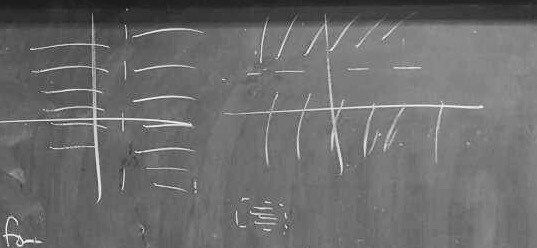
\includegraphics[scale=.3]{old_homework/topology_homework/half_planes}
\end{subfigure}
\end{figure}
\end{example*}
\begin{proof}(Trevor's proof) Let $\B$ be the collection of all finite interesections of $\script{S}$. 
\begin{itemize}
\item $\emptyset\in\B$, since $\set{x>1}\cap\set{x<1}=\emptyset$. 
\item $\B$ covers $X$, since $\set{x>0}\cup\set{x<1}=X$.
\item $\B$ is closed under finite intersections by assumption. 
\end{itemize}
So, by Thm 13, $\script{S}$ is a subbasis for $(\R^2, usual)$. 
\end{proof}

%It's rather convenient that we have the above proof, since the general proof is very similar. 

\pagebreak

\begin{highlight}
\begin{theorem}
Let $X$ be a set, with $\script{S}$ as a collection of subsets of $X$. 

$\script{S}$ forms a subbasis for some topology on $X$ iff
\begin{enumerate}[label=(\alph*)]
\item There are $V_1 \ldots V_n \in \script{S}$ with $\emptyset=V_1\cap \ldots\cap V_n$. \\
(That is, there is a finite subcollection of disjoint sets in $\script{S}$.)
\item For every $x\in X$, there is $V\in\script{S}$ with $x\in V$. \\
(That is, $\script{S}$ covers $X$. )
\end{enumerate}
\end{theorem}
\end{highlight}

\begin{proof}
Given $\script{S}$ as described, define $\B$ to be the collection of all finite intersections of sets from $\script{S}$. We need to show that $\B$ is a basis for a topology, using Thm 13. 
\begin{enumerate}[label=(\alph*)]
\item $\emptyset\in\B$ since $\emptyset=V_1\cap\ldots\cap V_n$, thus $\emptyset$ is a finite intersection of sets in $\script{S}$. 
\item Since $\script{S}\subset\B$ and $\script{S}$ covers $X$, then $\B$ also covers $X$. That is, $\forall x\in X, \exists B\in\B$ such that $x\in B$. 
\item Suppose that we have $x\in B_1\cap B_2$, with $B_1, B_2\in \B$. This means that both $B_1$ and $B_2$ are finite intersections of sets in $\script{S}$. So, $B_1\cap B_2$ is also a finite intersection of sets in $\script{S}$, so $B_1\cap B_2\in\B$. Now we can take $B_x$ to be $B_1\cap B_2$, so we have $x\in B_x \subset B_1\cap B_2\in\B$. 
\end{enumerate}
\end{proof}

\section{Homeomorphisms}

\begin{highlight}
\begin{definition*}
Let $X$ and $Y$ be spaces. A \emph{homeomorphism} is a continuous bijection $f:X\to Y$, with $\inv{f}$ also continuous.
\end{definition*}
\end{highlight}

\begin{definition*}
If there is a homeomorphism between $X$ and $Y$, we say $X$ and $Y$ are \emph{homeomorphic}, and write $X\cong Y$. 
\end{definition*}

\begin{example*}
Consider the identity function $f:(\R,discrete)\to(\R,usual)$. In this case, $f$ is a bijection which is continuous, since the preimage of every open set is open. However, $\inv{f}$ is not continuous, so these two space are not homeomorphic. 
\end{example*}

\begin{example*}\textbf{(1)}\\
In $(\R,usual)$: $\R\cong (-\frac{\pi}{2},\frac{\pi}{2}).$ \\
This is true because $\tan: (-\frac{\pi}{2},\frac{\pi}{2})\to \R$ is a continuous bijection with a continuous inverse, $\arctan$. Note: we are implying that we mean for $(-\frac{\pi}{2},\frac{\pi}{2})$ to have the subspace topology in $(\R,usual)$. 
\end{example*}

\begin{example*}\textbf{(2)}\\
$(a,b)\cong (0,1)$. (usual topology)\\
Consider $f:(0,1)\to (a,b)$ such that $f(t)=(1-t)a+tb$. By the way, the same function shows that $[a,b]\cong [0,1]$.
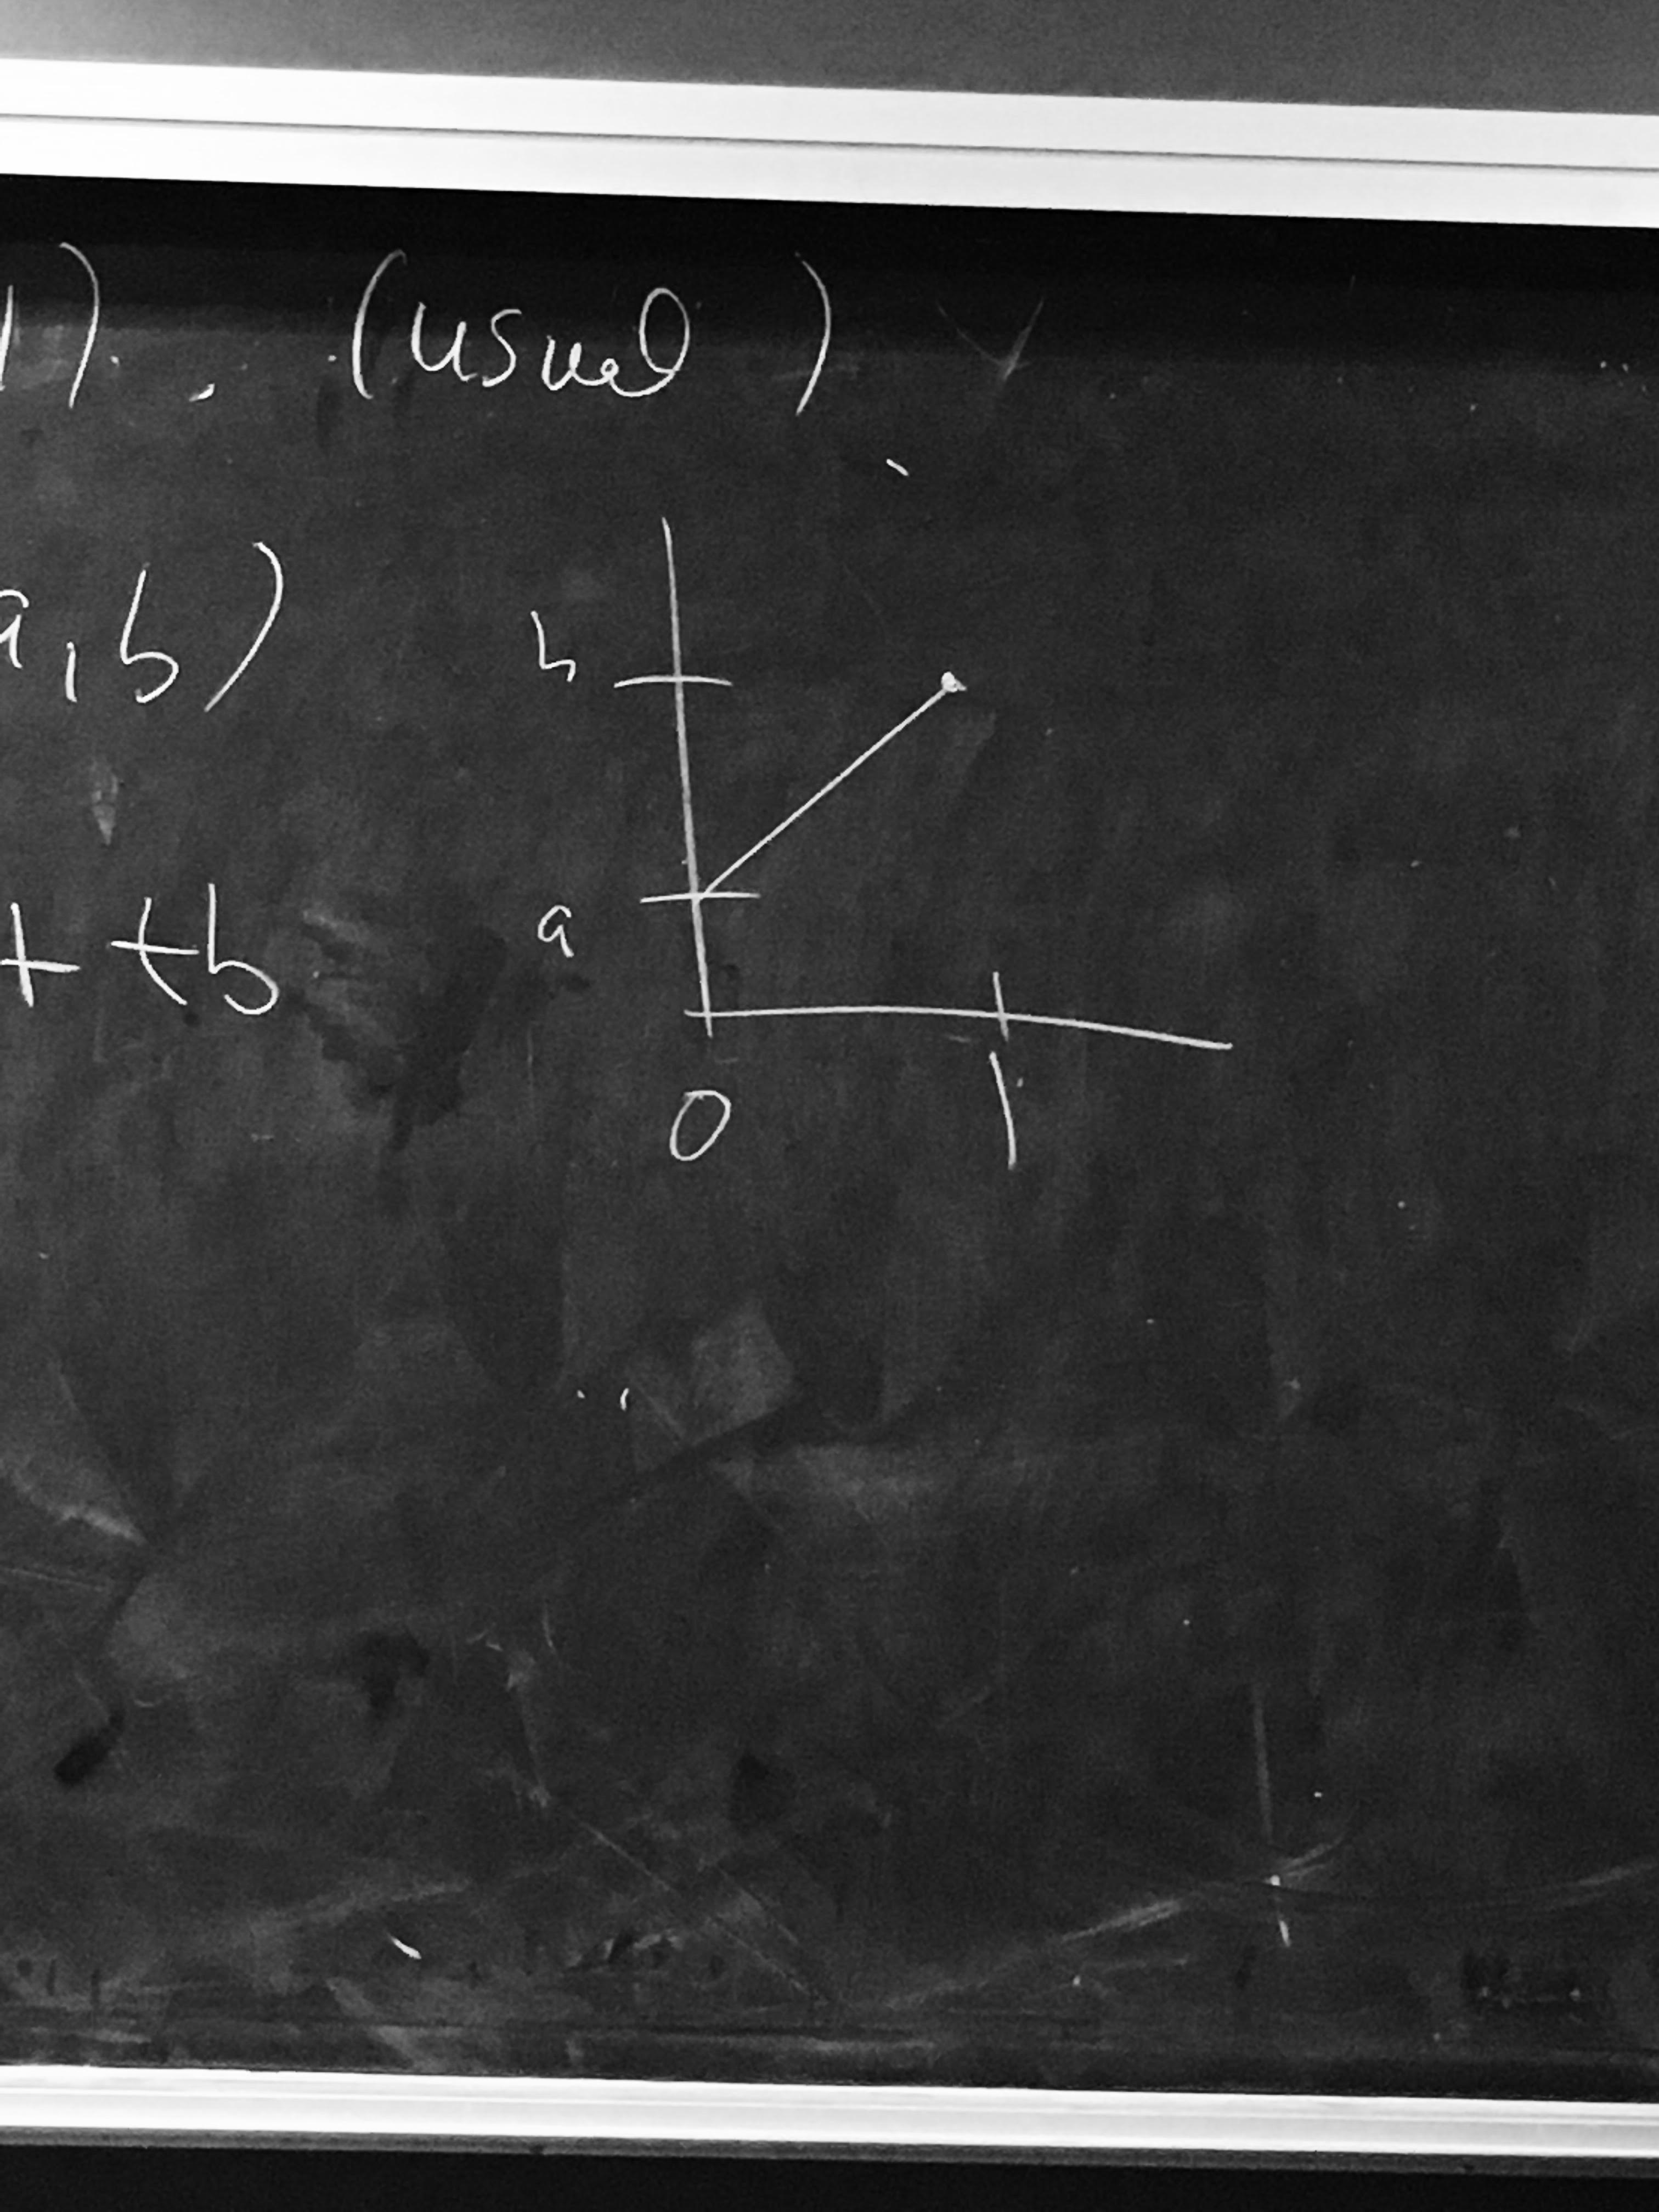
\includegraphics[scale=.02]{images/ab_01_homeomorph}
\end{example*}

\begin{remark*}
Examples (1) and (2) together show that $\R\cong (a,b), \forall a<b\in\R$. 
\end{remark*}

\begin{example*}\textbf{(3)}\\
$(\R, usual)$ is homeomorphic to $X=\{(x,0):x\in\R\}\subset(\R^2, usual)$. 

Consider $f:\R \to X$. Such that $f(x)=(x,0)$, and $\inv{f}(x,0)=x$. Now, $\inv{f}$ is continuous, because $\inv{(\inv{f})}(a,b)=f(a,b)=X\cap B(\frac{a+b}{2},\frac{b-a}{2})$. $f$ is continuous because every basic open set in $X$ is of the form $B((x_0,y_0),r)\cap X=\{(x,0):a<x<b\},$ for some $a,b$ and $\inv{f}(B(x_0,y_0),r)\cap X)=(a,b)$. 

\begin{center}
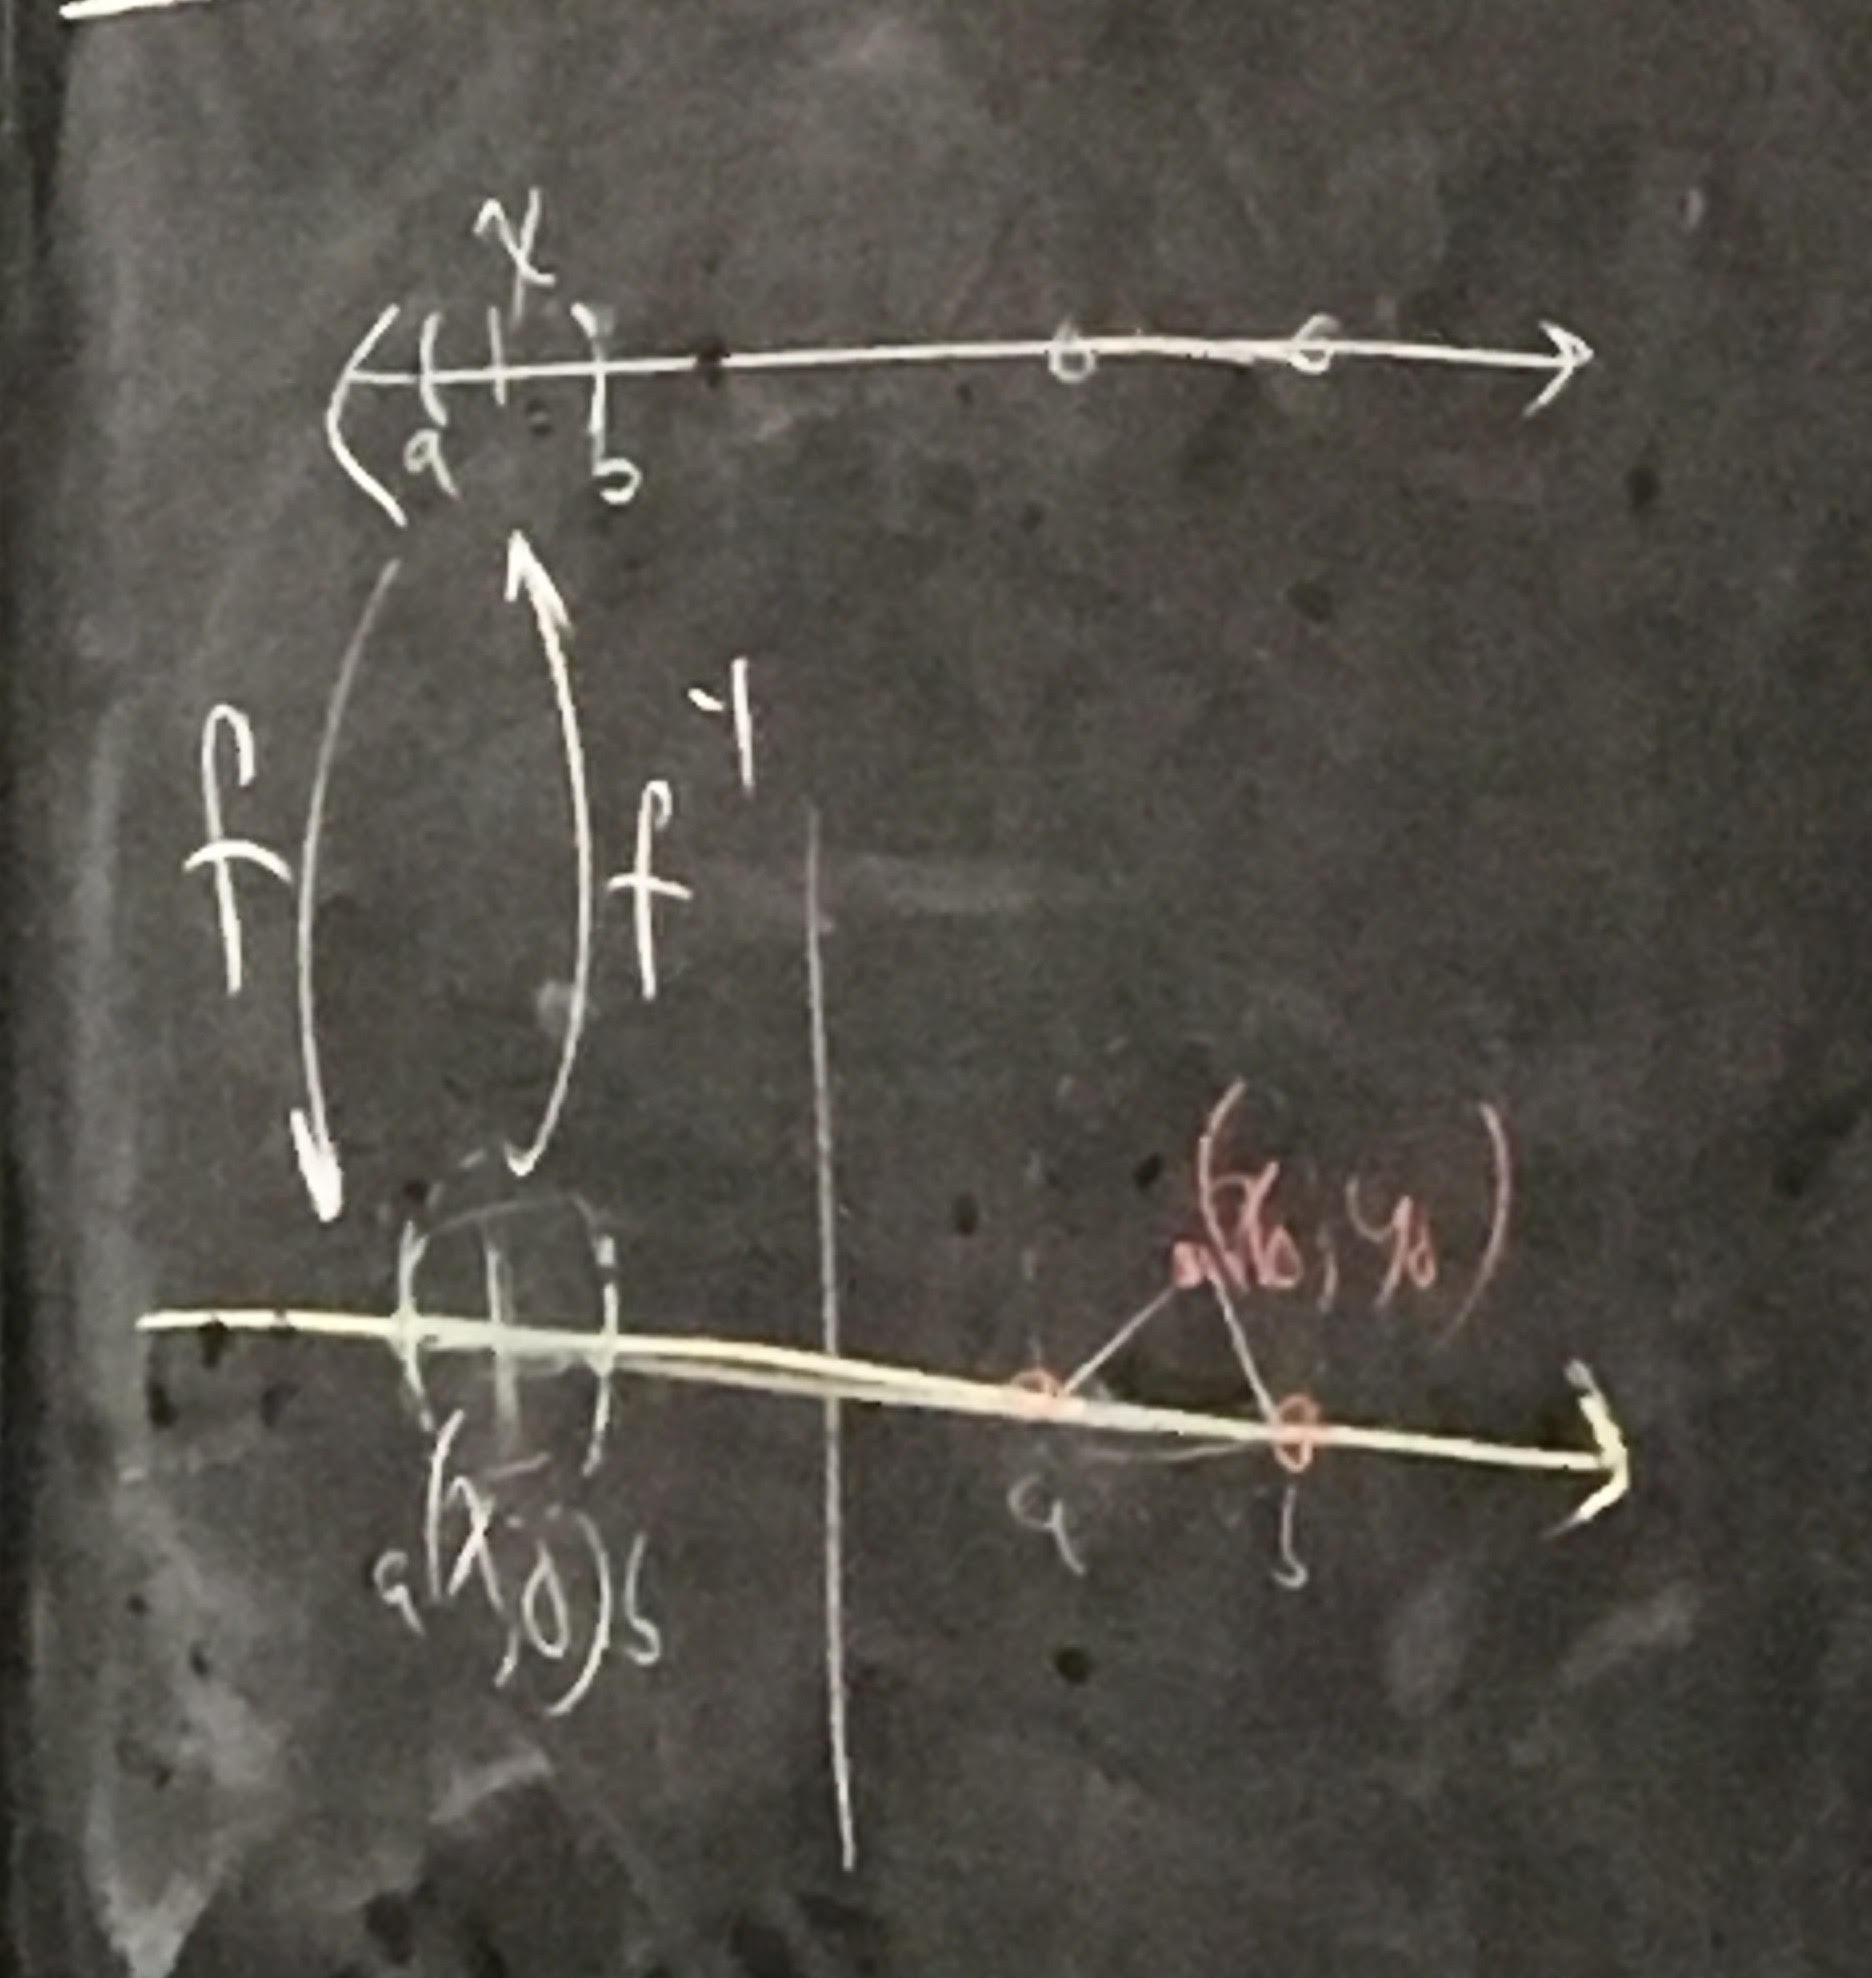
\includegraphics[width=3in, height=1.5in]{images/line_r2_r_homeo}
\end{center}
\end{example*}


\begin{example*}\textbf{(4)}
Let $S=\{(x,y):x^2+y^2=1\}\in\R^2$. Let $T=\{(x,y):|x|=1\text{ or } |y|=1\}$ in $\R^2$. 

\begin{center}
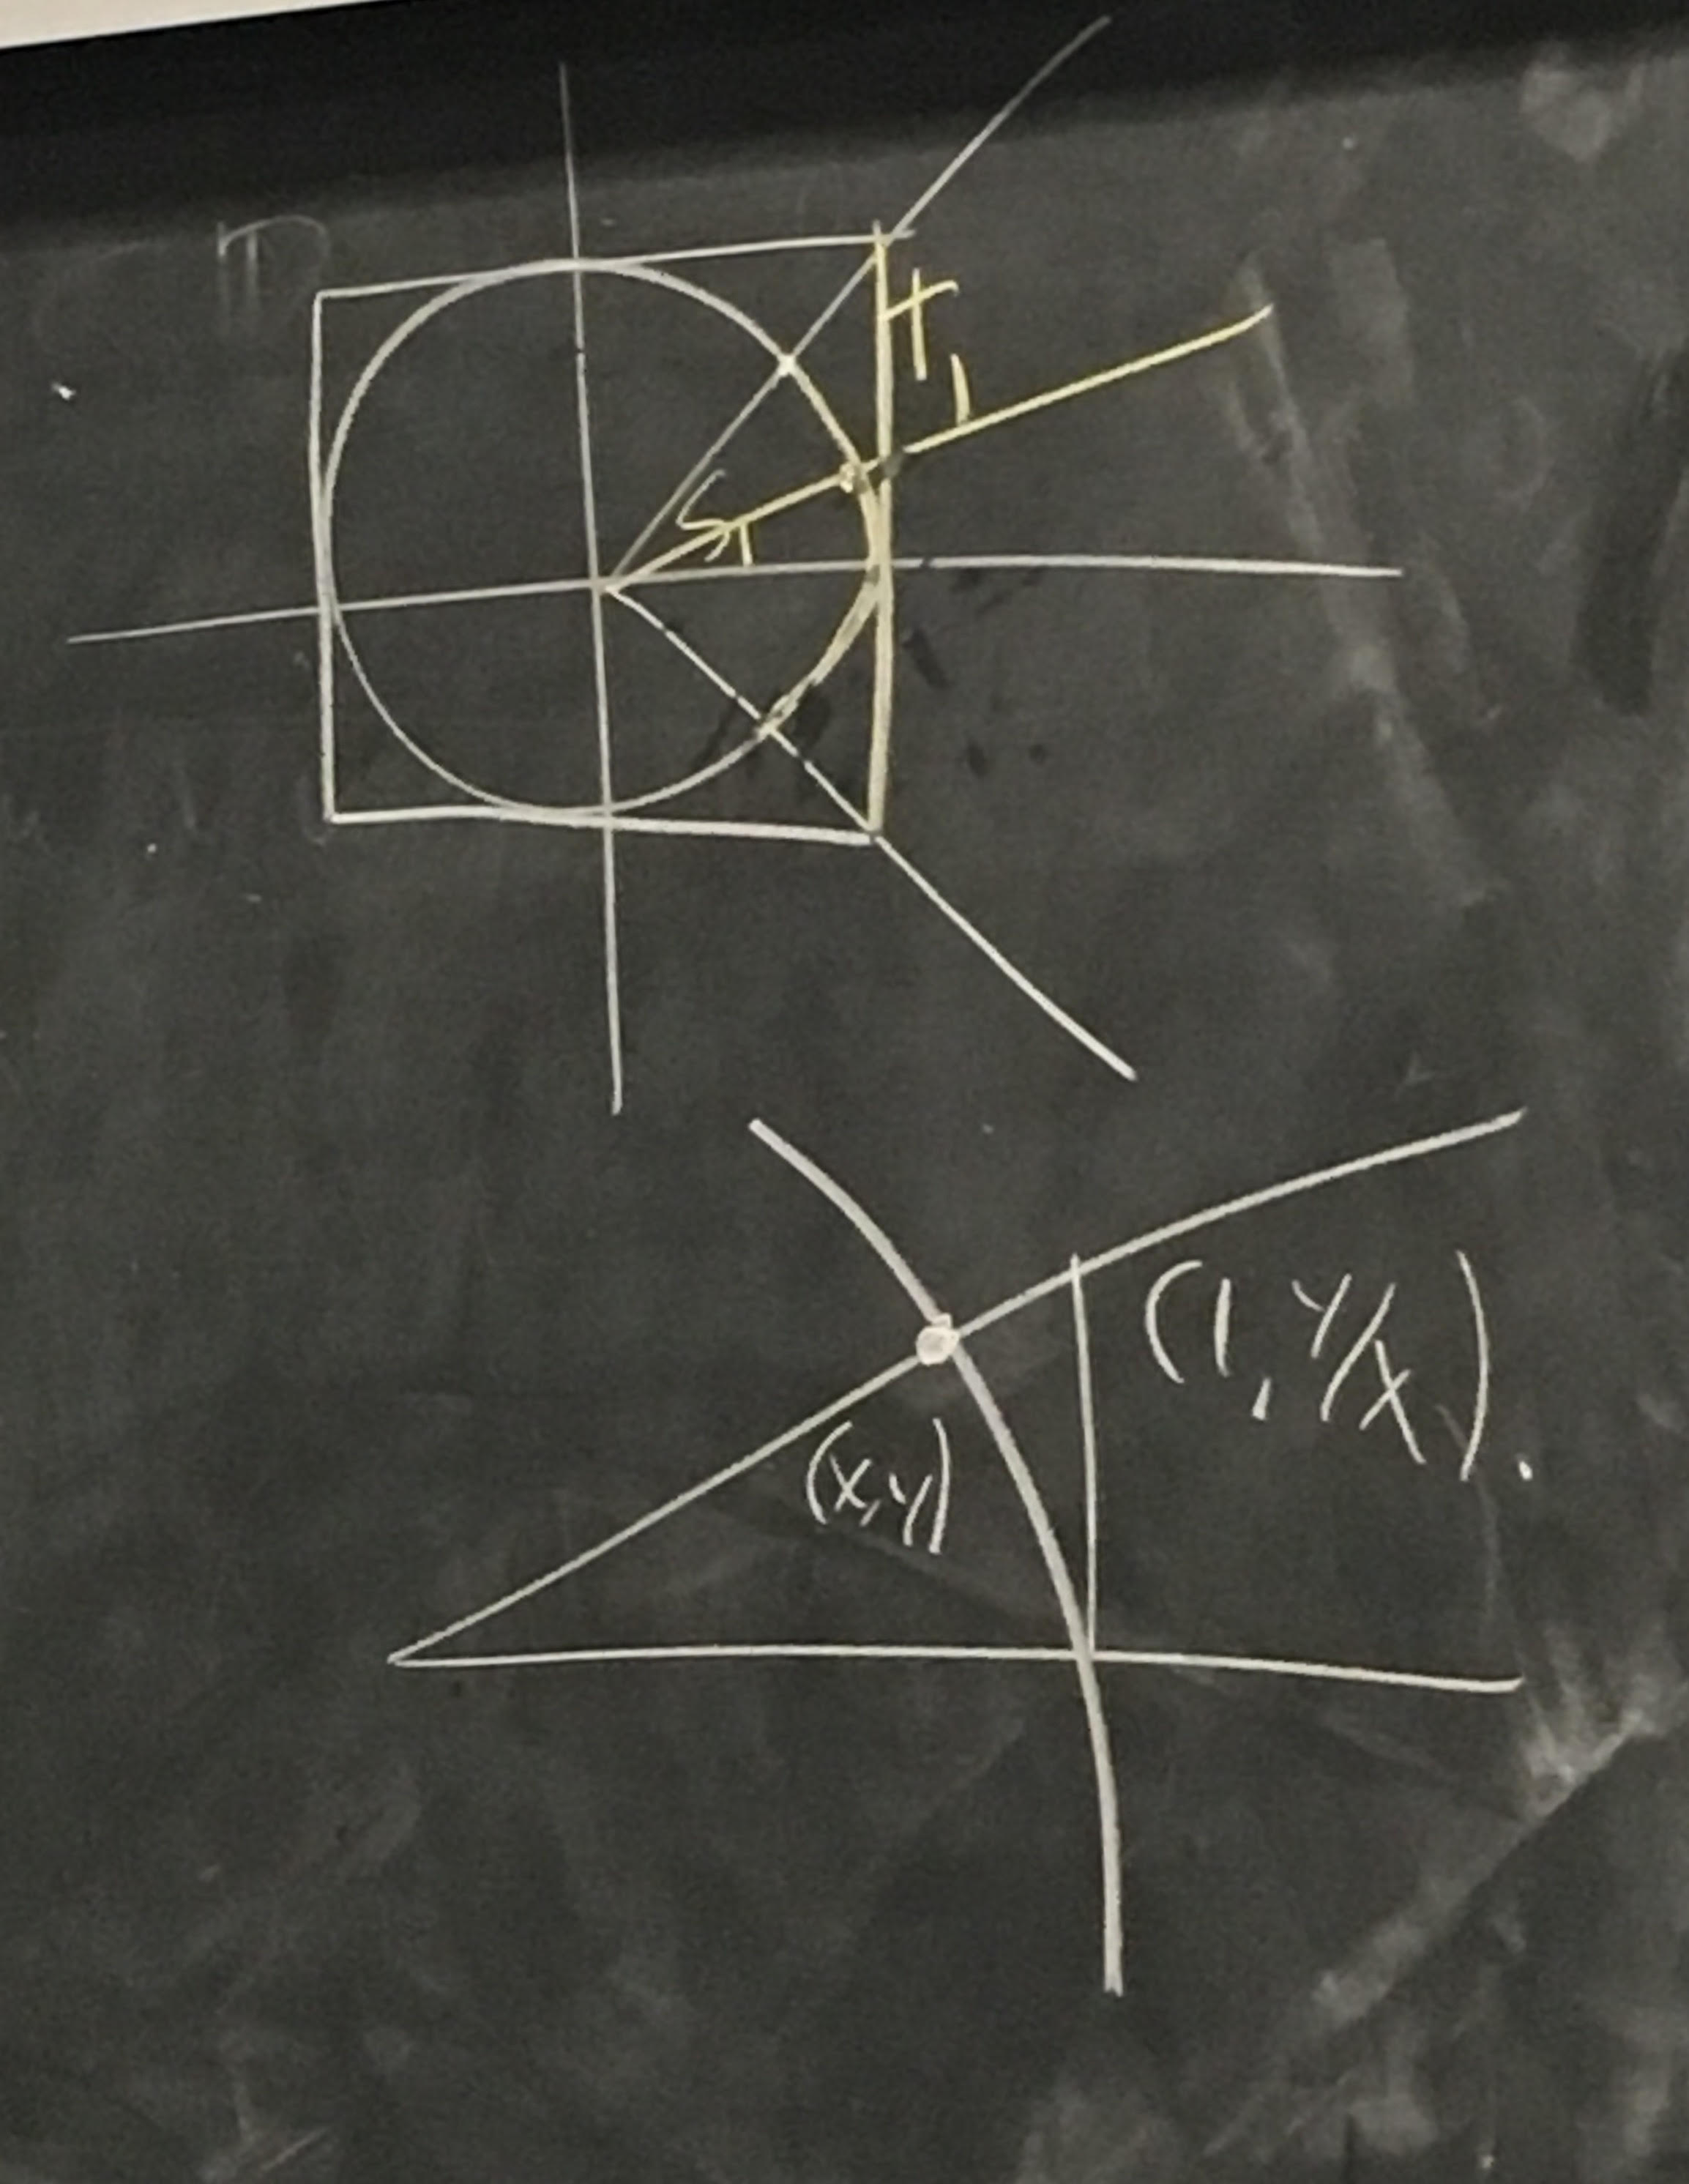
\includegraphics[scale=.04]{images/s_t_figs}
\end{center}

$f_1:S_1\to T_1$ such that $f_1(x,y)=(1,\frac{y}{x})$. 
$g_1:T_1\to S_1$ such that $g_1(u,v)=(\frac{u}{\sqrt{u^2+r^2}},\frac{v}{\sqrt{u^2+r^2}})$.

It is easily checked that these are inverses of each other, and they are continuous because they are restrictions of continuous functions. 

Similarly, we can define $f_i:S_i\to T_i, i=2,3,4$. 

By the Piecing Lemma (prop 10 i think?), together they give a homeomorphism $f:S\to T$. 
\end{example*}

\begin{example*}\textbf{(5)}\\
Let $S$ denote the unit circle centered at the origin. $S-\{(0,1)\}$ is homeomorphic to $\R$ (We're going to think of $\R$ as the $x$-axis in $\R^2$).

\begin{center}
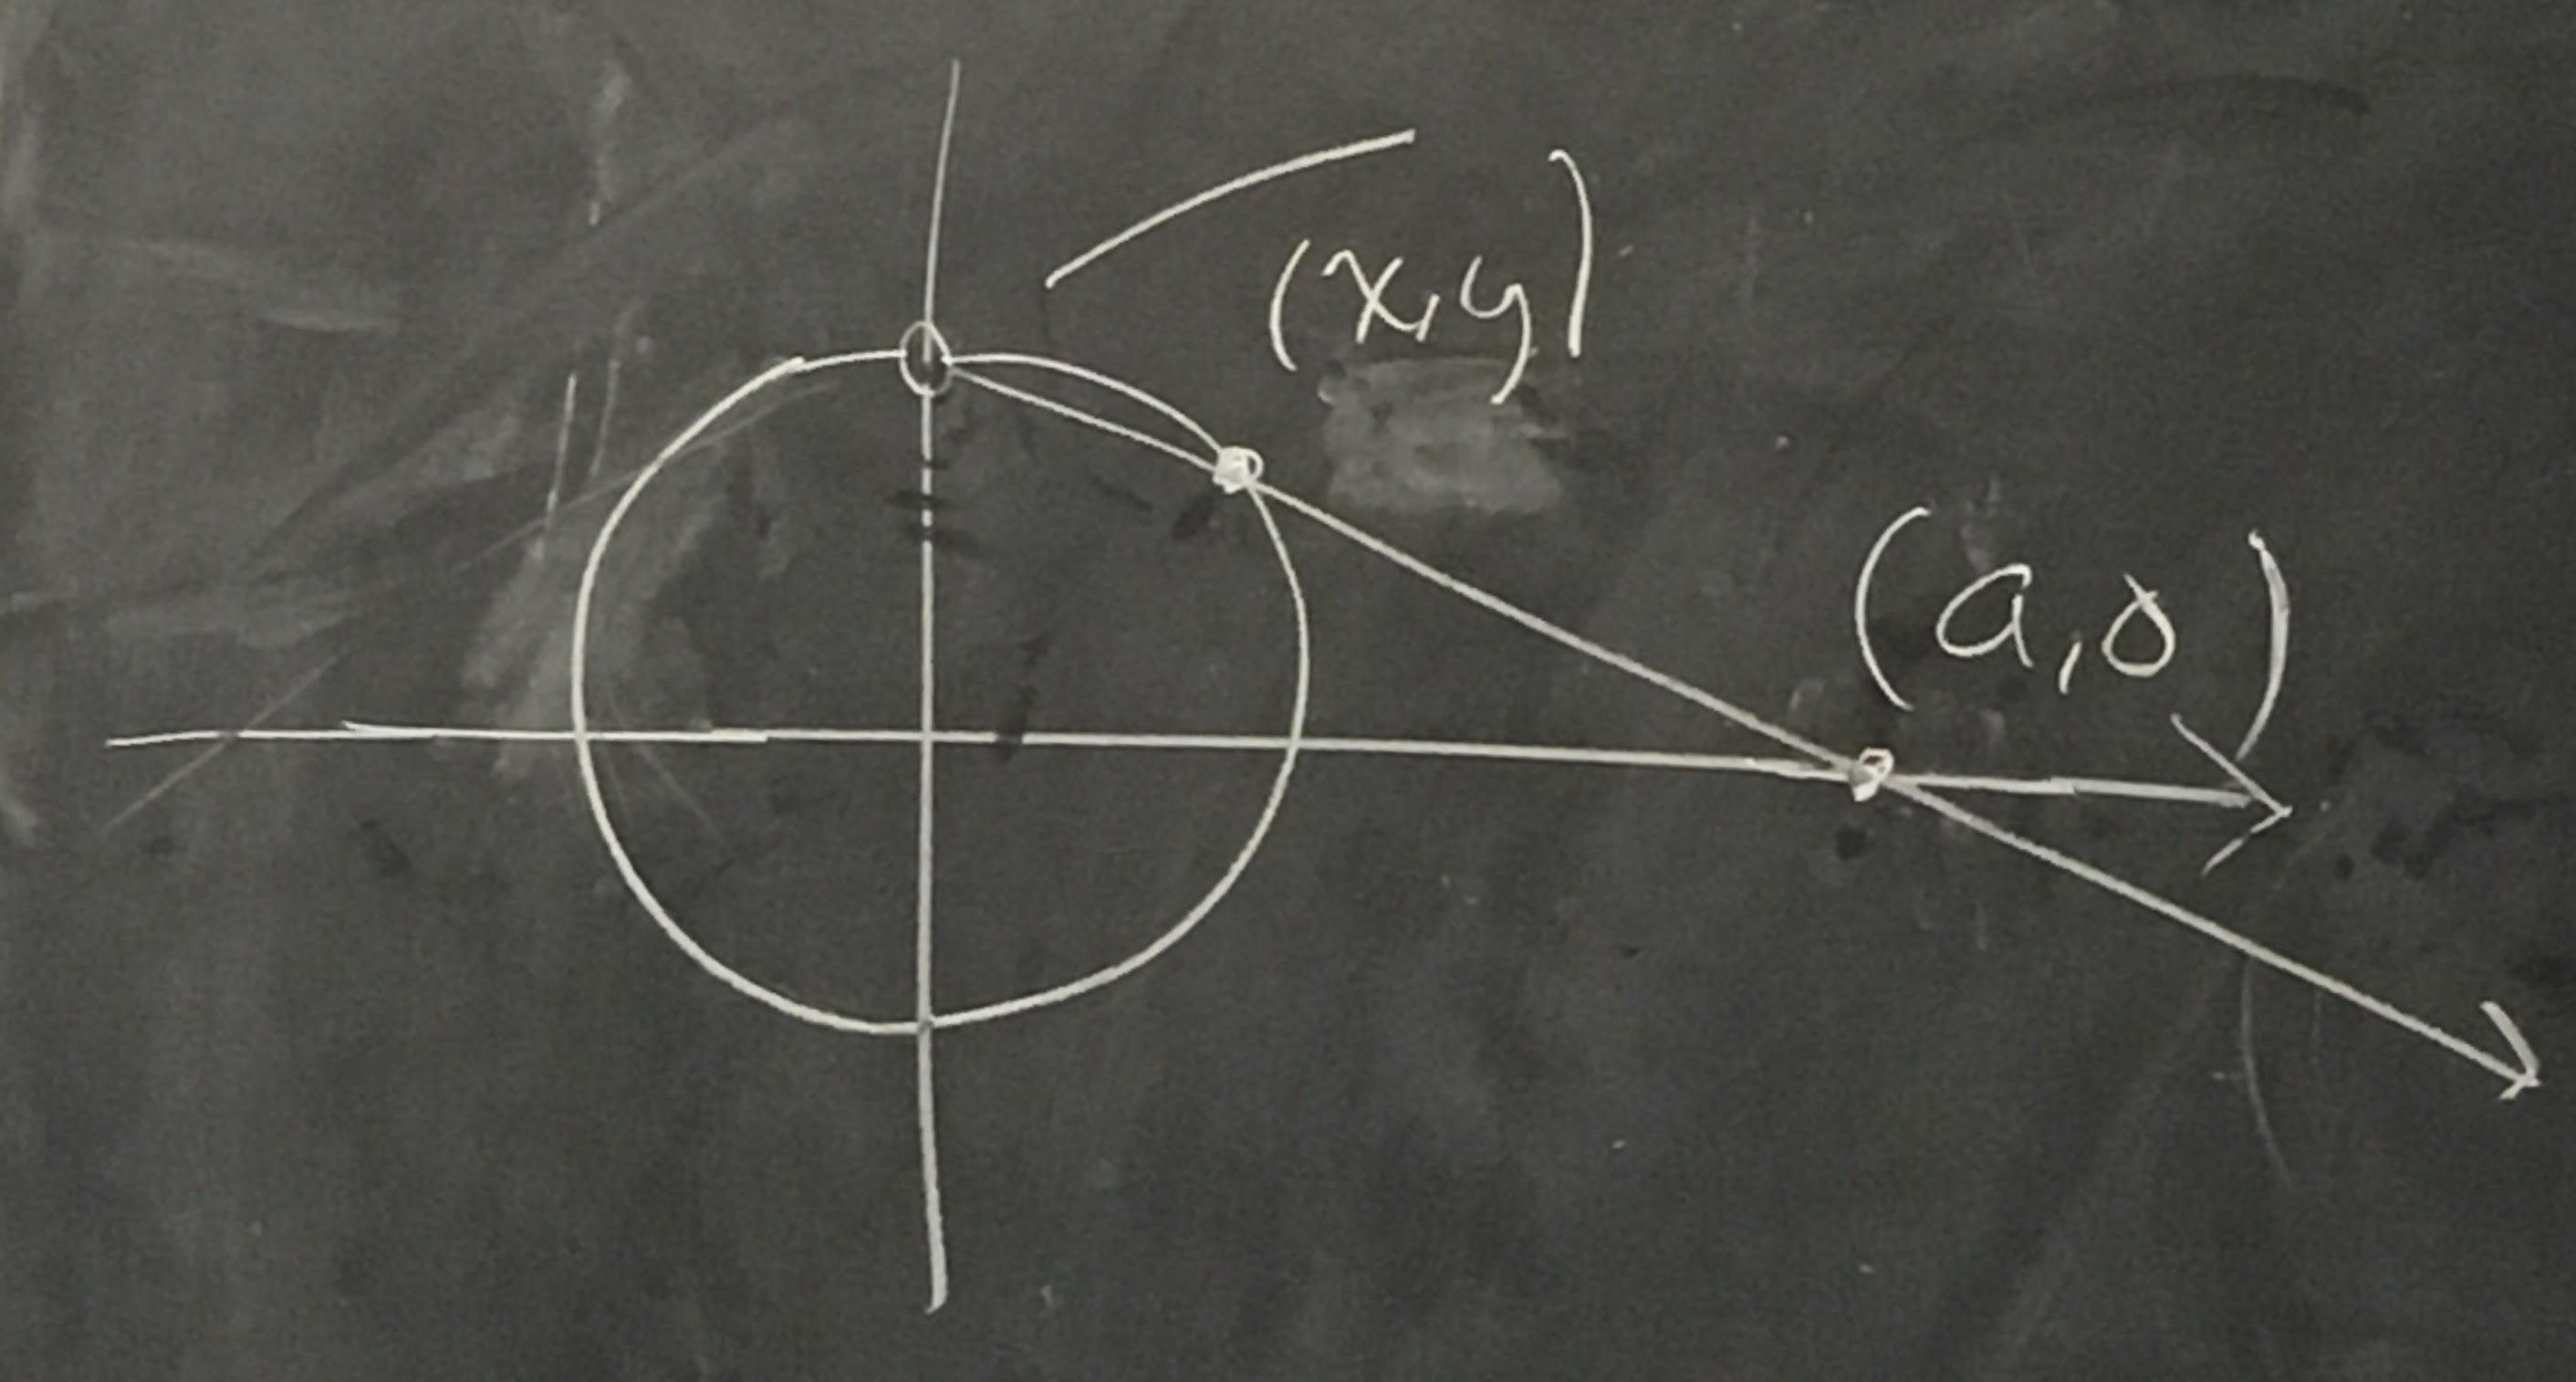
\includegraphics[scale=.07]{images/s_circ_projec}
\end{center}

Let $f:S-\{(0,1)\}\to \R$ such that $f((x,y))=(\frac{x}{1-y	},0)$. 

We also have $g:\{x\text{-axis}\}\to S-\{(0,1)\}$ such that $g(a,0)=\left(\frac{2a}{a^2+1}, \frac{a^2-1}{a^2+1}\right)$

It can be checked that $(g\circ f)(x,y)=(x,y),$ and $(f\circ g)(u,0)=(u,0),$ so $f$ and $g$ are bijections. $f$ and $g$ are continuous, because they are restrictions of continuous functions of $\R^2-\{y=1\}$ and $\R^2$, respectively. 
\end{example*}

\section{Compactness}

\begin{definition*}
Let $X$ be a space or subspace. A collection $\{U_\alpha\}_{\alpha\in\Gamma}$ of open sets is an \emph{open cover} of $X$ is $X\subseteq\arbcup{U}$. 
\end{definition*}

\begin{definition*}

If $\arbcoll{U}$ is a cover of $A\subset X$, then a $\emph{subcover}$ of $\arbcoll{U}$ is a subcollection $\{U_\alpha\}_{\alpha\in\Gamma'}$ for some $\Gamma'\subset\Gamma$ which is also an open cover of $A$. 

\end{definition*}

\begin{highlight}
\begin{definition*}
Let $X$ be a space. $X$ is \emph{compact} if every open cover of $X$ has a finite subcover. 

A subset $A\subset	X$ is a \emph{compact subset} of $X$ ($X$ may or may not be compact) if every open cover of $A$ (by open sets in $X$) has a finite subcover. 
\end{definition*}
\end{highlight}

\begin{proposition*}
Let $A$ be a subset of a topological space $X$. The following are equivalent:
\begin{itemize}
	\item $A$ is a compact subset of $X$. 
	\item $A$ is a compact space with regard to the subspace topology in $X$. 
\end{itemize}
\end{proposition*}
\begin{proof}\mbox{}\\
($\impliedby$) Suppose $A$ is a compact space. and $A\subset \arbcoll{U}$, with all $U_\alpha$ open in $X$. But then 
$A=A\cap(\arbcoll{U})=\arbcoll{A\cap U}.$
So since $A$ is a compact space, there is a finite subcover of $\arbcoll{A\cap U}$, which implies that $\arbcoll{U}$ also covers $A$. So, $A$ is a compact subset of $X$.

\noindent ($\implies$) Suppose $A$ is a compact subset of $X$. let $A=\arbcoll{V}$ with all $V_\alpha$ open in $X$. By definition, each $V_\alpha=A\cap U_\alpha$, with $U_\alpha$ open in $X$. So $A\subset \arbcup{U}$. Since $A$ is a compact subset of $X$, we have $A\subset \bigcup U_{\alpha i}$, so then $A=A\cap \bigcup U_{\alpha i}=\bigcup(A\cap U_{\alpha i})=\bigcup V_{\alpha i}$. 
\end{proof}

\begin{remark*}
You may have a set $A\subset X$, with $A$ compact. Don't let yourself say things like "$A$ is compact in $X$". This doesn't have much of a meaning, since a set $A$ is either compact or it isn't. It doesn't matter what the ambient space is. Another way to say this is, if $A$ is compact, then it is compact as subset of $X$, or as a subset of $Y$, or whatever else.
\end{remark*}

\begin{example*}\textbf{(1)}:\\
$(\R,usual)$ is not compact. Now, $\{(-n,n):n\in \N\}$ is an open cover with no finite subcover, since any finite subcollection has a set with greatest $n$, and that subcollection does not include $n+1$. 
\end{example*}

\begin{example*}\textbf{(2)}:\\
$(\R,finite\ complement)$ is compact. Suppose $\arbcoll{U}$ is an open cover of $\R$. Pick any $U_{\alpha_0}, \alpha_0\in\Gamma$. If $U_{\alpha_0}=\R$, then we are done. Otherwise, $U_{\alpha_0}=\R-\{a_1, \ldots a_N\}, a_i\in \R$. Now, each $a_1, \ldots a_N$ is in some other open set $U_{\alpha_i}$, and $\bigcup\limits_{0\leq i \leq K} U_{\alpha_i}$ is our finite subcover. 
\end{example*}

\begin{example*}\textbf{(3)}:\\
$[a,b)$ is not a compact subset of $(\R, usual)$, since $\{(a-1,b-\frac{1}{n}):n\in\N\}$ is an open cover of $[a,b)$, but any finite subcollection leaves out the point $\{b-\frac{1}{\max(n)+1}\}$. 
\end{example*}

\begin{highlight}
\begin{theorem}
$[a,b]$ is a compact subset of $(\R, usual)$.
\end{theorem}
\end{highlight}
\begin{proof}
Let $\arbcoll{U}$ be an open cover of $[a,b]$. Let $A=\{x\in[a,b] : \exists$ a finite subcover of $\arbcoll{U}$ for $[a,x]\}$. Now, $A\neq\emptyset$ because $a\in A$. \\
$a\in U_{\alpha_0}$, for some $\alpha_0$. Now, $A$ is bounded above by $b$. So, let $u=\sup A$. \\
\textbf{Claim:} $u=b$. To see this, suppose $u<b$. We know that $u\in U_{\alpha_1}$ for some ${\alpha_1}$.
\end{proof}

\subsection{Results Involving Compactness}

\begin{highlight}
\begin{proposition}
Suppose $X,Y$ are spaces, where $X$ is compact, and $f:X\to Y$ is continuous. Then, $f(X)$ is a compact subset of $Y$. 
\end{proposition}
\end{highlight}
\begin{proof}
Let $\arbcoll{V}$ be an open cover of $f(X)$. Then, $\{\inv{f}(V_\alpha)\}_{\alpha\in\Gamma}$ is an open cover of $X$. So, since $X$ is compact, it has a finite subcover $\inv{f}(V_{\alpha_1}), \ldots, \inv{f}(V_{\alpha_n})$. Now, $V_{\alpha_1}, \ldots, V_{\alpha_n}$ is a finite subcover of $f(X)$, because any $y\in f(X)$ is such that $y=f(x)\subset f(\inv{f}(V_{\alpha_k}))\subset V_{\alpha_k}$. 

\begin{center}
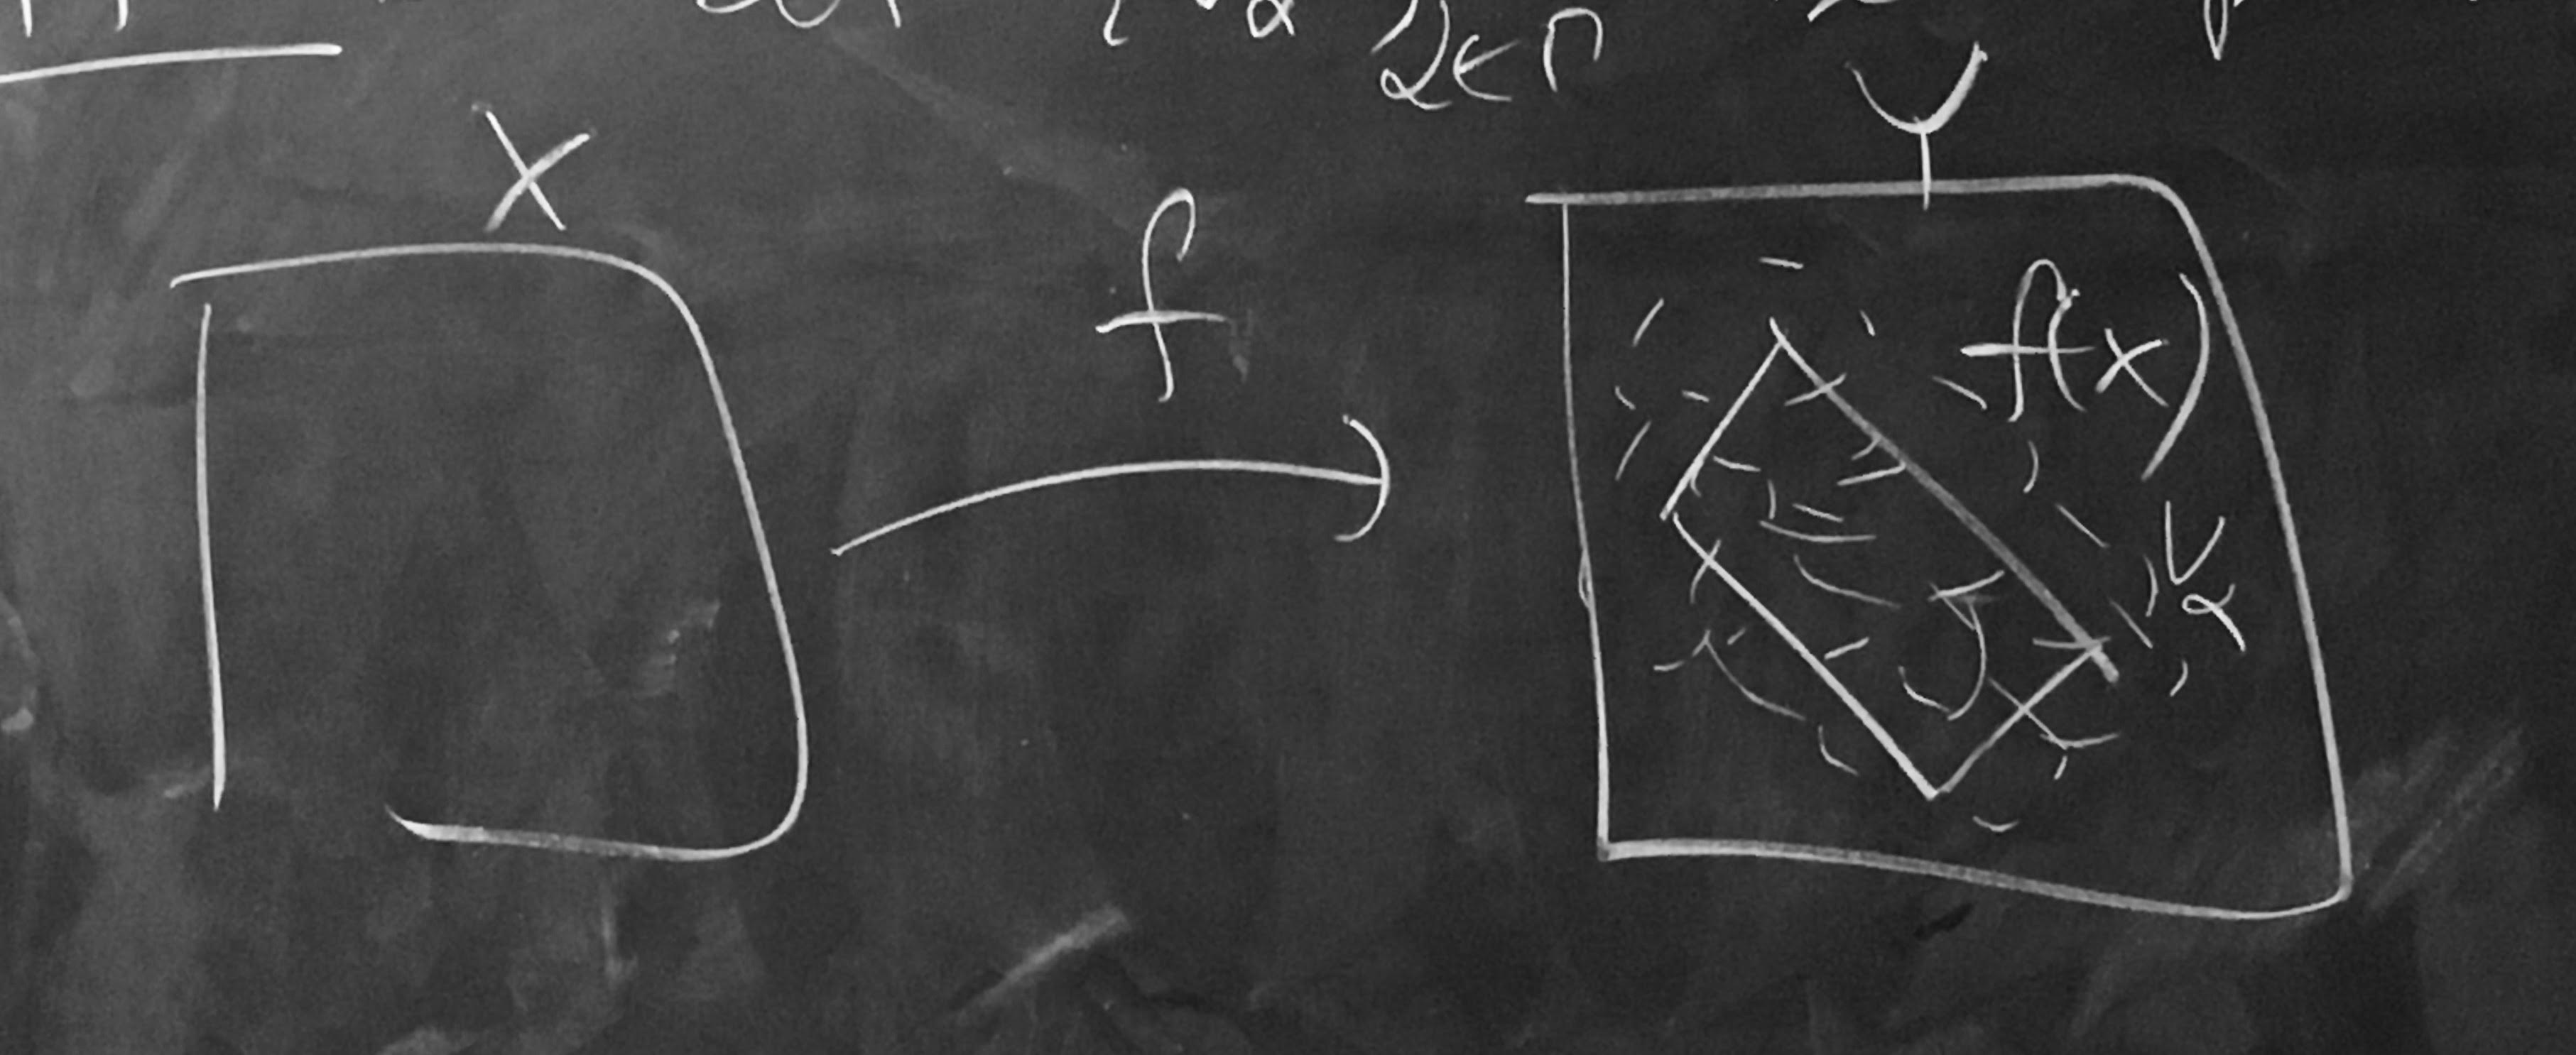
\includegraphics[scale=.06]{images/pf16_fig}
\end{center}

\end{proof}

\begin{highlight}
\begin{corollary}
Suppose $X,Y$ are spaces, where $X$ is compact, and $f:X\to Y$ is continuous and onto. Then, $Y$ is compact. 

In particular, if $f$ is a homeomorphism, then $Y$ is compact. That is, compactness is preserved by homeomorphisms. 
\end{corollary}
\end{highlight}

\begin{highlight}
\begin{theorem}
Let $X$ be a compact space, with $A$ a closed subset of $X$. Then, $A$ is a compact subset. (A closed subset of a compact space is compact.)
\end{theorem}
\end{highlight}
\begin{proof}
Let $\arbcoll{U}$ be an open cover of $A$. Then, $\arbcoll{U}\bigcup(X-A)$ is an open cover of $X$. Since $X$ is compact, then this cover has a finite subcover $U_{\alpha_1}, \ldots, U_{\alpha_n}, X-A$. In particular, $U_{\alpha_1}, \ldots, U_{\alpha_n}$ is a finite subcover of $A$. 

\begin{center}
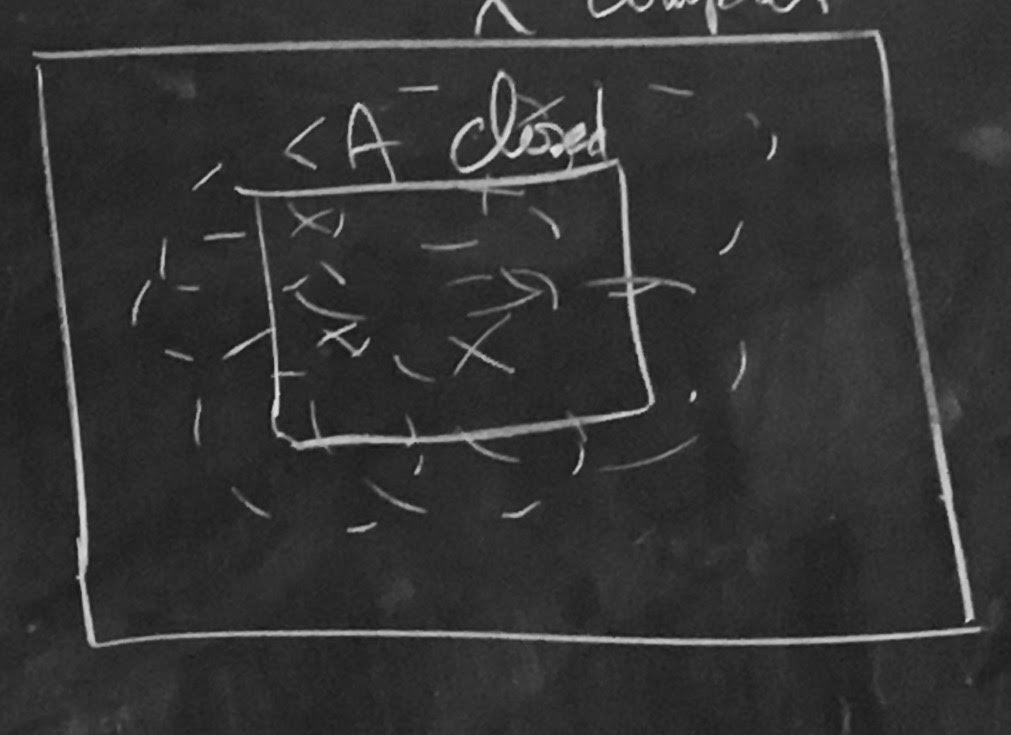
\includegraphics[scale=.12]{images/thm18_fig}
\end{center}

\end{proof}

\begin{highlight}
\begin{theorem}
Let $X$ be Hausdorff, with $A$ a compact subset of $X$. Then, $A$ is closed. (A compact subset of a Hausdorff space is closed.)
\end{theorem}
\end{highlight}
\begin{proof}
Let $x\in X-A$ be fixed. For every $y\in A$, there exist open sets $U_y$, $V_x$ with $y\in U_y$, $x\in V_y$, $U_y\cap V_y = \emptyset$. Now, $\{U_y\}_{y\in A}$ is an open cover of $A$, so it has a finite subcover $U_{y_1}\ldots U_{y_n}$. Let $V = V_{y_1}\cap \ldots \cap V_{y_n}$. Now $V$ is open, and $x\in V$ by construction.
Claim: $V\cap A=\emptyset$. To see this, if not, then suppose $z\in V \cap A$. Then $z\in A$, so $z\in U_{y_k}$, but also $z\in V$ implies $z\in V_{y_k}$ which is a contradiction. \\
So we have $x\in V\subset X-A$. By the openness criterion, for any $x\in X-A$, there exists open $V$ such that $X\in V$, so $X-A$ is open and $A$ is closed. 
\end{proof}

\begin{definition*}
$A\subset\R$ is \emph{bounded} if there exists $N>0$ such that $|x|\leq N$ for all $x \in A$. 

Equivalently, $A$ is bounded if there exists $N>0$ with $A\subset [-N,N]$. 
\end{definition*}

\begin{definition*}\textit{(More general)}
Let $X$ be a metric space with metric $d$. We say $A\subset X$ is \emph{bounded} if there exists $x_0\in A$, and $N>0$ such that $A\subset \closure{B_d}(x_0,N)$. 

Equivalently, $A$ is bounded if there exists $x_0\in A$, and $N>0$ such that $d(x,x_0)\leq N$ for all $x\in A$. 
\end{definition*}

\begin{highlight}
\begin{theorem}[Heine-Borel Theorem]\mbox{}\\
Let $A\subset (\R, usual)$. Then, $A$ is compact iff $A$ is closed and bounded. 
\end{theorem}
\end{highlight}
\textit{Warning:} This equivalence is false in general. 
\begin{proof}\mbox{}\\
$\implies:$ If $A$ is compact, then $A$ is closed by Thm 19. To see that $A$ is bounded, note that $\{(-n,n)\}_{n\in\N}$ is an open cover of $A$, which must have a finite subcover. In fact, $A\subset (-N,N)$, for some $N\in\N$. \\
%
$\impliedby$: Suppose $A$ is closed and bounded. Since $A$ is bounded, $A\subset[-N,N]$, for some $N\in\N$. Now, $A$ is closed in $\R$, and $A=A\cap[-N,N]$, so $A$ is closed in $[-N,N]$. So, $A$ is a closed subset of a compact space, so by Thm 18, $A$ is compact in $[-N,N]$. It follows that $A$ is compact in $\R$:\\
Let $\arbcoll{U}$ be an open cover of $A$, open in $\R$. Since $A\subset [-N,N]$, $[-N,N]\cap\arbcoll{U}$ covers $A$. So, since $A$ is compact in $[-N,N]$, there exists a finite subcover $[-N,N]\cap \{U_n\}_1^{N'}$. Now, since $A\subset [-N,N]$, $\{U_n\}_1^{N'}$ still covers $A$. Thus, $A$ is compact in $\R$. 
\end{proof}

\begin{highlight}
\begin{theorem}
Let $X$ be compact space, and let $F:X\to (\R,usual)$ be continuous. Then, "$f$ attains its maximum and minimum." That is, there exists $x_0,x_1\in X$ such that $f(x_0)\leq f(x)$ for all $x\in X$ and $f(x)\leq f(x_1)$ for all $x\in X$. 
\end{theorem}
\end{highlight}
\begin{proof}
Since $X$ is compact, $f(X)$ is a compact subset of $\R$, so the image is bounded. Let $s=\inf f(X)$ and $t=\sup f(X)$. \\
Claim: $s,t\in f(X)$. \\
Note, $f(X)$ is closed by Heine-Borel. If $s\not\in f(X)$, then $s\in\R-f(X)$, so there exists $\epsilon>0$ such that $(s-\epsilon, s+\epsilon)\subset \R-f(X)$. However, $s+\frac{\epsilon}{2}\leq f(x)$ for all $x\in X$, so $s+\frac{\epsilon}{2}>s$ is also a lower bound for $f(X)$, which contradicts $s=\inf f(X)$. 
\end{proof}

\begin{definition*}
Let $X,Y$ be topological spaces. A continuous function $f:X\to Y$ is call an \emph{open} map or function if $f(U)$ is open for all open $U\subset X$. 
\end{definition*}

\begin{definition*}
Let $X,Y$ be topological spaces. A continuous function $f:X\to Y$ is call an \emph{closed} map or function if $f(K)$ is closed for all closed $K\subset X$. 
\end{definition*}

\begin{remark*}
A homeomorphism $f:X\to Y$ is 1-1, onto, and continuous by defintion. As a result, it is also both open and closed. 
\end{remark*}

\begin{highlight}
\begin{theorem}
Let $X,Y$ be topological spaces, and let $f:X\to Y$ be a function which is 1-1, onto, and continuous, with $X$ compact, and $Y$ Hausdorff. Then, $f$ is a homeomorphism. 
\end{theorem}
\end{highlight}
\begin{proof}
It suffices to show that $f$ is closed. Let $K\in X$ be closed. Since $X$ is compact, and $K$ is closed, then $K$ is compact. So $f(K)$ is compact, and is a subset of $Y$ which is Hausdorff. So $f(K)$ is closed by Thm 19. 
\end{proof}

\section{Metric Spaces}

\begin{definition*}
Let $X$ be any set. We say that a \emph{metric} is a function $d:X\times X \to \R^+$ such that 
\begin{enumerate}
\item $d(x,y)=0$ iff $x = y$. \\
(Definiteness)
\item $d(x,y)=d(y,x)\quad$ for all $x,y \in X$.\\
(Symmetric property)
\item $d(x,z) \leq d(x,y) + d(y,z) \quad$ for all $x,y,z \in X$. \\
(Triangle Inequality)
\end{enumerate}
Define $B_d(x,r)=\{y\in X : d(x,r)<r\}$.\\
$U \subset X$ is \emph{open} if for all $x \in U$, there is $r(x)>0$ such that $B_d(x,r(x))\subset U$. 
A proof similar to example (1) will show that this forms a topology on $X$. We say that these open sets comprise the topology on $X$ generated by $d$.
\end{definition*}

\begin{highlight}
\begin{theorem}[Lebesque's Lemma]\mbox{}\\
Let $X$ be a compact metric space, with metric $d$. Let $\arbcoll{U}$ be an open cover of $X$. Then, there exists a $\delta>0$ such that for all $x\in X$, we have that $x\in B(x,\delta)\subset U_{\alpha_x}$ for some $\alpha_x\in\Gamma$. 
\end{theorem}
\end{highlight}
\begin{proof}
For every $x\in X$, there is a $\delta_x$ such that $B(x,\delta_x)\subset U_{\alpha_x}$, for some $\alpha_x\in\Gamma$. Now, $\{B(x,\frac{\delta_x}{2})\}_{x\in X}$ is an open cover of $X$. Since $X$ is compact, $\{B(x,\frac{\delta_x}{2})\}_{x\in X}$ has a finite subcover, $B(x_1,\frac{\delta_{x_1}}{2})\ldots, B(x_n,\frac{\delta_{x_n}}{2})$. \\
Let $\delta=\min(\frac{\delta_{x_1}}{2}\ldots\frac{\delta_{x_n}}{2})$. \\
\\
Now we need to show that this works for any $x$. Let $x\in X$. We have $x\in B(x_k, \frac{\delta_{x_k}}{2})$, for some $k\in\{1\ldots n\}$. So, if $y\in B(x,\delta)$, then 
$$d(y,x_k) \leq d(y,x) + d(y,x_k)< \delta + \frac{\delta_{x_k}}{2} \leq \frac{\delta_{x_k}}{2} + \frac{\delta_{x_k}}{2} = \delta_k. $$
So $y\in B(x_k, \delta_{x_k})\subset U_{\alpha_{x_k}}$. This gives $B(x,\delta)\subset U_{\alpha_{x_k}}$.
\end{proof}

\begin{remark*}
Let $X,Y$ be metric spaces, with metrics $d_x, d_y$, respectively. $f:X\to Y$ continuous is equivalent to:\\
For every $x\in X$ and $\epsilon>0$, there is $\delta=\delta(\epsilon,x)>0$ such that \\
$d_x(x',x)<\delta$ implies that $d_y(f(x'),f(x))<\epsilon.$
\end{remark*}

\begin{highlight}
\begin{definition*}
Let $X,Y$ be metric spaces, with metrics $d_x, d_y$, respectively. $f:X\to Y$ is \emph{uniformly continuous} if for every $\epsilon>0$, there is $\delta>0$ such that for all $x_1, x_2\in X$, if $d_x(x_1,x_2)<\delta$, then $d_y(f(x_1),f(x_2))<\epsilon$.
\end{definition*}
\end{highlight}

\begin{highlight}
\begin{theorem}
Let $X,Y$ be metric spaces with metrics $d_x, d_y$, and $X$ compact. Then every continuous $f:X\to Y$ is uniformly continuous. 
\end{theorem}
\end{highlight}

\subsection{Convergence and Cauchy}

\begin{highlight}
\begin{definition*}
Let $X$ be a metric space, with metric $d$. \\
A sequence $(X_n)_{n=1}^\infty$ \emph{converges} to $x_0\in X$ if for every $\epsilon>0$, there is $N$ such that 
$$\forall n \geq N, \quad d(x_n, x_0)<\epsilon.$$
\end{definition*}

\begin{definition*}
Let $X$ be a metric space, with metric $d$. \\
A sequence $(X_n)_{n=1}^\infty$ is \emph{Cauchy} if for every $\epsilon>0$, there is $N$ such that 
$$\forall m,n \geq N, \quad d(x_m, x_n)<\epsilon.$$ 
\end{definition*}
\end{highlight}

\begin{highlight}
\begin{definition*}
Let $X$ be a metric space, with metric $d$. \\
We say $X$ is \emph{complete} (or \emph{d-complete}) if every Cauchy sequence in $X$ converges to a point in $X$ (with respect to $d$). 
\end{definition*}
\end{highlight}

\begin{example*}(1)
$\R$ together with $d(x,y)=|x-y|$ is complete. \\
However, $\R$ together with $d(x,y)=|\arctan x-\arctan y|$ is \emph{not} complete. For example, consider $(n)_{n=1}^\infty$. 
\end{example*}

\begin{example*}(2)
Consider $\Q$ with subspace topology of $(\R,usual)$. $d(x,y)=|x-y|.$ This is not complete, since $(3.14, 3.141, 3.1415, \ldots)$ is a Cauchy sequence which does not converge to a rational. 
\end{example*}

\begin{example*}(3)
Consider $(0,1)$ as a subspace of $(\R,usual)$, together with the usual metric. This space is not complete. For example, $(\frac{1}{n})_{n=1}^\infty$ is Cauchy but does not converge in $(0,1)$. 
\end{example*}

\begin{highlight}
\begin{theorem}
Let $X$ be a compact metric space with metric $d$. Then, $X$ is complete. 
\end{theorem}
\end{highlight}
\begin{proof}
Let $(x_n)_{n=1}^\infty$ be Cauchy. We can find $N$ such that $d(X_m,X_n,)<\frac{\epsilon}{2}$, for all $m,n\geq N$. Consider the set $A={x_n}_{n=1}^\infty$. 

If $A$ is finite, let $0<\lambda<\min(d(x_i-x_j))$. Since the sequence is Cauchy, by taking $\epsilon=\delta$, we see that there is some $N$ such that $X_m=X_n$ for all $m,n>N$. (We say the sequence is \emph{eventually constant} in this case.) So certainly this Cauchy sequence convergerges to $x_N$. 

If $A$ is infinite, then since $X$ is compact, then $A$ has a limit point $x_0$. Furthermore, there exists $M>N$ such that $d(x_m, x_0)<\frac{\epsilon}{2}$. To see this, note that if not, let $$\lambda=\min(\{\frac{\epsilon}{2}\}\cup \{d(x_1,x_0), \ldots d(x_N,x_0):d(x_k,x_0)\neq0\})$$. Then, $B(x_0,\lambda)-\{x_0\}\cap A \neq \emptyset$, contradicting that $x_0$ is a limit point. Now, for $n\geq N$, $$d(x_n, x_0) \leq d(x_n,x_m)+d(x_m,x_0)<\frac{\epsilon}{2}+\frac{\epsilon}{2}=\epsilon.$$ 
\end{proof}

\begin{highlight}
\begin{proposition}
If $X$ is a metric space with complete metric $d$, and $A\subset X$ is closed, then $A$ with metric $d$ is complete. 
\end{proposition}
\end{highlight}
\begin{proof}
Let $(x_n)_{n=1}^\infty$ be a Cauchy sequence in $A$. Since $X$ is complete with respect to $d$, there exists $x\in X$ with $(x_n)_{n=1}^\infty$ converging to $x$. But, $x$ is a limit point of $A$, and since $A$ is closed, $x\in A$. 
\end{proof}

\subsection{Baire Category Theorem}

Recall the following facts from earlier:
\begin{definition*}
A set $A$ is \emph{dense} in $X$ if $\closure{A}=X$.
\end{definition*}
\begin{proposition*}
A subset $A$ is dense in $X$ if and only if for all $U$ open in $X$, we have $U\cap A\neq\emptyset$. That is, every open set contains an element of $A$. 
\end{proposition*}

\begin{highlight}
\begin{theorem}[Baire Category Theorem]
Let $X$ be a complete metric space, with metric $d$. If $\{U_i\}_{i=1}^\infty$ is a collection of dense open sets, 
$$\bigcap_{i=1}^\infty U_i \text{ is dense.}$$
\end{theorem}
\end{highlight}
\begin{proof}
To prove this theorem, it suffices to show that for all $x\in X, \epsilon>0$, we have $B(x,\epsilon)\cap (\bigcap_{n=1}^\infty U_n)\neq\emptyset$. Since $U_1$ is dense, there is $x_1\in U_1\cap B(x,\epsilon)$. Sicne $U_1$ is open, we can find $r_1>0$ such that $B(x_1,r_1)\subset U_1\cap B(x,\epsilon)$. 
\end{proof}

\begin{example*}
To see why completeness is necessary, Consider $\Q$ with $d_{usual}$. We know $\Q$ is countable,

(I didn't finish typing this proof)
\end{example*}

\begin{definition*}
For $X$ space, a $A\subset X$ is called \emph{nowhere dense} if $\text{int}(\closure{A})=\emptyset$. 
\end{definition*}

\begin{proposition*}
A set is nowhere dense iff $X-\closure{A}$ is dense.
\end{proposition*}

\begin{highlight}
\begin{corollary}[Baire Category Theorem version 2]
Let $X$ be a complete metric space, with metric $d$. $X$ is not a countable union of nowhere dense closed sets. 
\end{corollary}
\end{highlight}

\section{Product Topology of Spaces}

\begin{definition*}
Let $X,Y$ be sets. The set of all ordered pairs $X\times Y = \{(x,y):x\in X,y\in Y\}$ is called the \emph{Cartesian product} of $X$ and $Y$. 
\end{definition*}

\begin{highlight}
\begin{definition*}
Let $X,Y$ be sets. The collection of sets $U\times V$ with $U$ open in $X$ and $V$ open in $Y$ forms the basis for a topology on $X\times Y$ (You can prove this). 

This collection is called the \emph{product topology} on $X\times Y$. 
\end{definition*}
\end{highlight}

\begin{exercise}
(For fun) What is the product topology of $\R^1_\text{bad}\times\R^1_{usual}$?
\end{exercise}

\begin{definition*}
Given spaces $X,Y$, we have projection functions as follows:
$$\pi_X:X\times Y \to X \quad \pi_X(x,y)=x$$
$$\pi_Y:X\times Y \to Y \quad \pi_X(x,y)=y$$

We also have inclusion functions as follows:
$$ \text{For all } x\in X, i_x:Y\to X\times Y \quad i_x(y)=(x,y)$$
$$ \text{For all } y\in Y, i_y:X\to X\times Y \quad i_y(x)=(x,y)$$
\end{definition*}

\begin{proposition}
Given spaces $X,Y$ and $X\times Y$ with the product topology, then $\pi_X, \pi_Y, i_x \forall x\in X, i_y \forall y\in Y$ are all continuous. 
\end{proposition}
\begin{proof}
The proof follows directly from the definitions. The preimage of an open set is open. You can do the proof if you have to. 
\end{proof}

\begin{corollary}\mbox{}\\
$X\cong X\times {y}$ for any $y\in Y$. \\
$Y\cong \{x\}\times Y$ for any $x\in X$. 
\end{corollary}
\begin{proof}
For any $y$, $\pi_X$ is a homeomorphism between $X$ and $X\times\{y\}$ with inverse $i_y$. Similiarly, for any $x$, $\pi_Y$ is a homeomorphism between $X$ and $X\times\{x\}$ with inverse $i_x$. 
\end{proof}

\begin{highlight}
\begin{proposition}
Suppose $X,Y$ are Hausdorff. Then, $X\times Y$ is Hausdorff. 
\end{proposition}
\end{highlight}
\begin{proof}
Exercise.
\end{proof}

\begin{highlight}
\begin{theorem}
Suppose $X,Y$ are compact. Then $X\times Y$ is compact. 
\end{theorem}
\end{highlight}
\begin{proof}
Let $\arbcoll{W}$ be an open cover of $X\times Y$. Fix $x\in X$. Now, $\arbcoll{W}$ is an open cover of $\{x\}\times Y$. Since $\{x\}\times Y$ is compact, then this has a finite subcover $W_{x,\alpha_1}, W_{x,\alpha_1}, \ldots, W_{x,\alpha_n(x)}$. Let $W_x=\bigcup_{i=1}^{n(x)} W_{x,\alpha_i}$. Notice that for all $y\in Y$, there are open sets $U_y$ in $X$, $V_y$ in $Y$ with $(x,y)\in U_y\times V_y\subset W_x$. The collection $\{U_y\times V_y\}_{y\in Y}$ is an open cover of $\{x\}\times Y$, so it has a finite subcover $U_{y_1}\times V_{y_1}, \ldots, U_{y_r}\times V_{y_r}$. Let $U_x=\bigcap_{i=1}^r U_{y_i}$. Notice $U_x\times Y \subset W_x$.\\

Now observe that we can produce a $U_x$ for every $X\in X$. So, $\{U_x\}_{x\in X}$ is an open cover of $X$. Since $X$ is compact, there is a finite subcover $\{U_{x_i}\}_{i=1}^p$. Now, $\{U_{x_i}\times Y\}_{i=1}^p$ covers $X\times Y$. So, since each $U_x\times Y \subset W_x$ for all $x$, then $\{W_{x_i}\times Y\}_{i=1}^p$ covers $X\times Y$. But, recall that each $W_{x}=\bigcup_{i=1}^{n(x)} W_{x,\alpha_i}$. However, ${W_{x_j,\alpha_i} : 1\leq j \leq p, 1\leq i\leq n(x_j)}$ is finite, so we have a finite subcover. 
\end{proof}

We now prove the Heine-Borel Theorem again using our new tools, and the proof is much simpler. 
\begin{theorem}[Heine-Borel Theorem]\mbox{}\\
Let $A\subset\R^n_{usual}$. $A$ is compact if and only if $A$ is closed and bounded. 
\end{theorem}
\begin{proof}
Suppose $A$ is compact. $\R^n$ being Hausdorff implies that $A$ is closed. To see that it is bounded, consider the open cover $\{B(0,n):n\in\N\}$. 

Conversely, suppose $A$ is closed and bounded. Since $A$ is bounded, $A\subset [a_n,b_1, \ldots [a_n,b_n]$, and thus it is compact by Thm 32. Now $A$ is a closed subset of a compact space, so $A$ is compact by Thm 18. 
\end{proof}

\pagebreak
\section{Compactification}

\begin{highlight}
\begin{definition*}
Let $X$ be a Hausdorff space. The \emph{one-point compactification topology} $\tilde{X}$ is defined as 
$$\tilde{X}=X\cup\infty.$$
%We define a topology on $\tilde{X}$ as follows:\\
$U$ is open in $\tilde{X}$ if either 
\begin{enumerate}[label=(\alph*)]
\item $U\subset X$ and $U$ is open in $X$, or 
\item $\infty\in U$, and $\tilde{X}-U$ is compact in $X$. 
\end{enumerate}
\end{definition*}
\end{highlight}

\begin{example*}
$\widetilde{\R^1}=\R^1\cup \{\infty\}$. 
\end{example*}

\noindent \emph{Claim:} $\widetilde{\R^1}$ is homeomorphic to $S^1$ (recall $S^1=\{(x,y)\in \R^2 : x^2+y^2=1\}$). 
\begin{proof}
Define $f:S^1 \to \widetilde{\R^1}$ by 
$$f(x,y)=
\begin{cases}
\left( \frac{x}{1-y}, 0 \right) & \text{if }(x,y)\neq(0,1)\\
\infty & \text{if } (x,y)=(0,1)
\end{cases}_.
$$
$f$ is a bijection. We know $S^1$ is compact, and we will see that $\widetilde{\R^1}$ is Hausdorff, so by Theorem 22, it is sufficient to confirm that $f$ is continuous. 

Now suppose $U$ is open in $\widetilde{\R^1}$ of type (b). By def, 
$$\widetilde{\R^1}-U=k,$$
where $k$ is compact in $\R^1$. We want to confirm that $\preimage{f}{U}$ is open in $S^1$. 
$$S^1-\preimage{f}{U}=\preimage{f}{\widetilde{\R^1}-U}=\preimage{f}{k},$$
and $k$ is compact. Now, $\inv{f}|_\R$ is known to be continuous, so $\preimage{f}{k}$ is a compact subset of $S^1$. Thus, $\preimage{f}{k}$ is closed be Theorem 18. So, f$f(U)$ is open in $S^1$ since we have already confirmed $f|_{S^1-(0,1)}$ is continuous. 
\end{proof}

\begin{highlight}
\begin{definition*}
A space $X$ is \emph{locally compact} if for all $x\in X$, there is an open set $U$ containing $x$ with $\closure{U}$ compact. 
\end{definition*}
\end{highlight}

(Example: $\R^n, usual$)

\begin{proposition}
Let $X$ be a locally compact Hausdorff space. Then, $\widetilde{X}$ is a compact Hausdorff space. 
\end{proposition}
\begin{proof}
(I need to copy this from my notes still.)
\end{proof}

\section{Separation Properties}

\begin{highlight}
\textbf{Separation Properties}
\begin{enumerate}
\item $X$ is $T_1$ (or \emph{Dumbledorff}) if for all $x,y\in X$, there is $U$ containing $x$ with $U\cap \{y\}=\emptyset$. Important note: this is equivalent to "singleton sets are closed". 
\item $X$ is \emph{Hausdorff} if for all $x,y\in X$ there are open sets $U$ containing $x$, $V$ containing $y$, with $U\cap V=\emptyset$. 
\item $X$ is \emph{regular} if for all $x\in X$ and all closed sets $A$ with $x\not\in A$, there exist open sets $U,V$ with $X\in U$, $A\subset V$, and $U\cap V=\emptyset$. 
\item $X$ is \emph{normal} if for all disjoint closed sets $A,B$, there exist open sets $U,V$ with $A\subset U, B\subset V, U\cap V=\emptyset$. 
\end{enumerate}
\end{highlight}

\begin{remark*}\mbox{}
\begin{itemize}
\item Normal + $T_1$ implies regular.
\item Regular + $T_1$ implies Hausdorff.
\end{itemize}
\end{remark*}

\begin{highlight}
\begin{theorem}
If $X$ is a metric space, then $X$ is normal. 
\end{theorem}
\end{highlight}
\begin{proof}
Let $A$ and $B$ be closed sets with $A\cap B =\emptyset$. Since $B$ is closed, for every $a\in A$, there is $r_a$ with $B(a,r_a)\cap B = \emptyset$. Simlilarly, for every $b\in B$, there is $r_b$ with $B(b,r_b)\cap A = \emptyset$. Let $U=\bigcup_{a\in A}B(a,\frac{r_a}{2}), V=\bigcup_{b\in B}B(b,\frac{r_b}{2})$. Now clearly $A\subset U, B\subset V$. 

\begin{center}
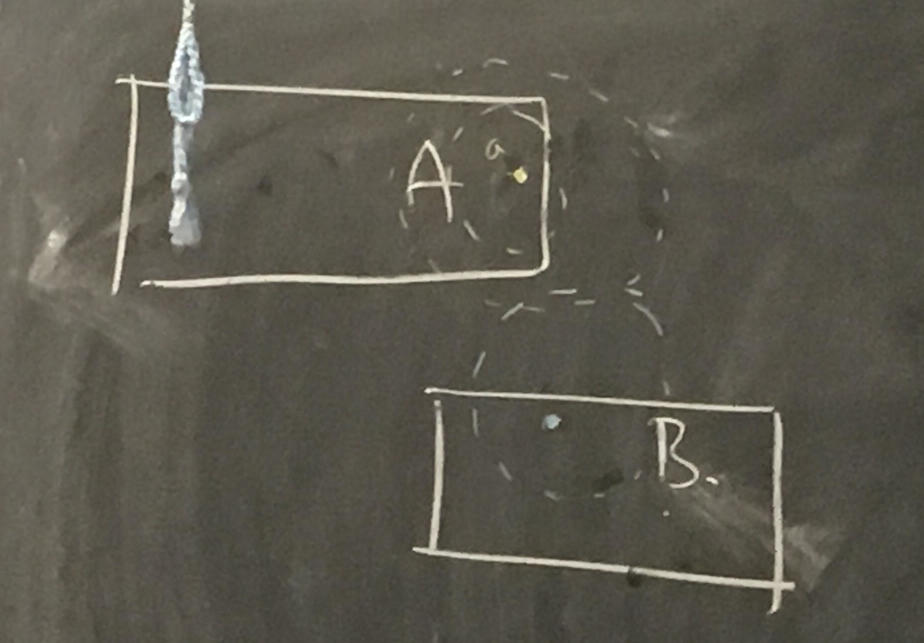
\includegraphics[scale=.12]{images/separation_1}
\end{center}

To see that $U\cap V=\emptyset$, suppose $z\in U\cap V$. Since $z\in U$, we have $z\in B(a,\frac{r_a}{2})$ for some $a\in A$, and also $z\in B(b,\frac{r_b}{2})$ for some $b\in B$. Now, 
$$d(a,b)\leq d(a,z)+d(z,b)< \frac{r_a}{2}+\frac{r_b}{2} <\max\{r_a,r_b\}.$$
If, say, $\max\{r_a,r_b\}=r_b$, this says that $a\in B(b,r_b)$, which is a contradiction. 
\end{proof}

\begin{highlight}
\begin{theorem}
If a space $X$ is compact and Hausdorff, then $X$ is normal.
\end{theorem}
\end{highlight}
\begin{proof}
We first show that $X$ is regular. Let $A$ be a closed set with $y\not\in A$. For every $a\in A$, there are open sets $U_a, V_a$, with $a\in U_a, y\in V_a, U_a\cap V_a = \emptyset$. 

\begin{center}
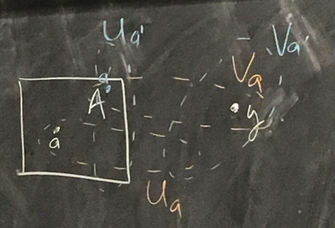
\includegraphics[scale=.4]{images/separation_2}
\end{center}

Note $\{U_a\}_{a\in A}$ is an open cover of $A$, so it has a finite subcover $U_{a_1}, \ldots U_{a_n}$. Let 
$$U=\bigcup_{i=1}^n U_{a_i}, \quad V=\bigcap_{i=1}^n V_{a_i}. $$
To see that $U\cap V=\emptyset$, suppose $z\in U\cap V$. Now, $z$ is in some $U_{a_k}$ for some k and $V_{a_i}$ for every $i$, so in particular, it is also in $V_{a_k}$, which is a contradiction.\qedwhite

Now we show that $X$ is normal. Let $A,B$ be disjoint closed sets. For for all $b\in B$, by regularity, we can find open sets $U_b, V_b$ with $A\subset U_b, b\in V_v, U_B\cap V-b=\emptyset$. $\{V_b\}_{b\in B}$ is an open cover of $B$ (and $B$ is compact), so it has a finite subcover, $V_{b_1}, \ldots V_{b_n}$. Let 
$$U=\bigcap_{j=1}^n U_{b_j}, \quad V=\bigcup_{j=1}^n V_{b_j}. $$
Now, $U\cap V=\emptyset$ as before. 
\end{proof}

\begin{highlight}
\begin{proposition}
$X$ is normal if and only if for any closed set $A$ and open set $U$ with $A\subset U$, there exists an open set $V$ with 
$$A\subset V \subset \closure{V} \subset U.$$
\end{proposition}
\end{highlight}
\begin{center}
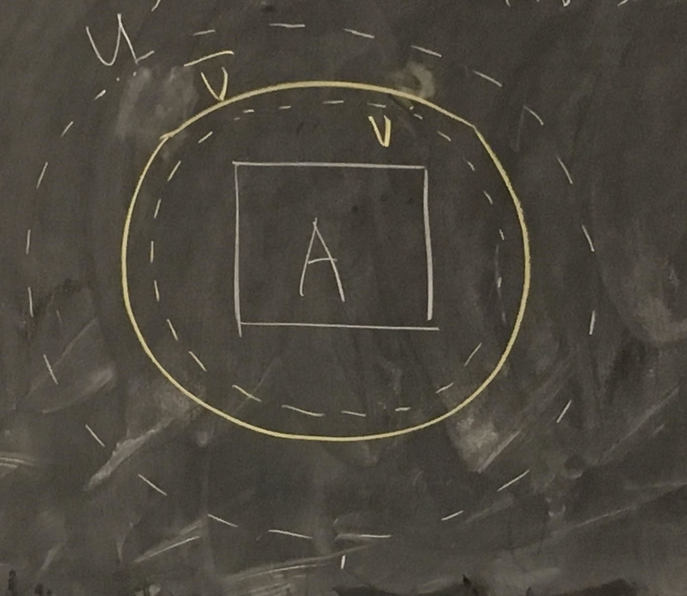
\includegraphics[scale=.16]{images/separation_3}
\end{center}
\begin{proof}
homework.
\end{proof}

\subsection{Urysohn's Lemma and Tietze's Extension Theorem}
\begin{highlight}
\begin{theorem}[Urysohn's Lemma]
Suppose $X$ is normal, and $A$ and $B$ are disjoint closed sets. Then there exists a continuous function $f:X\to [0,1]$ with the following property:
$f(a)=0$ for all $a\in A$, and $f(b)=1$ for all $b\in B$. 
\end{theorem}
\end{highlight}
\begin{center}
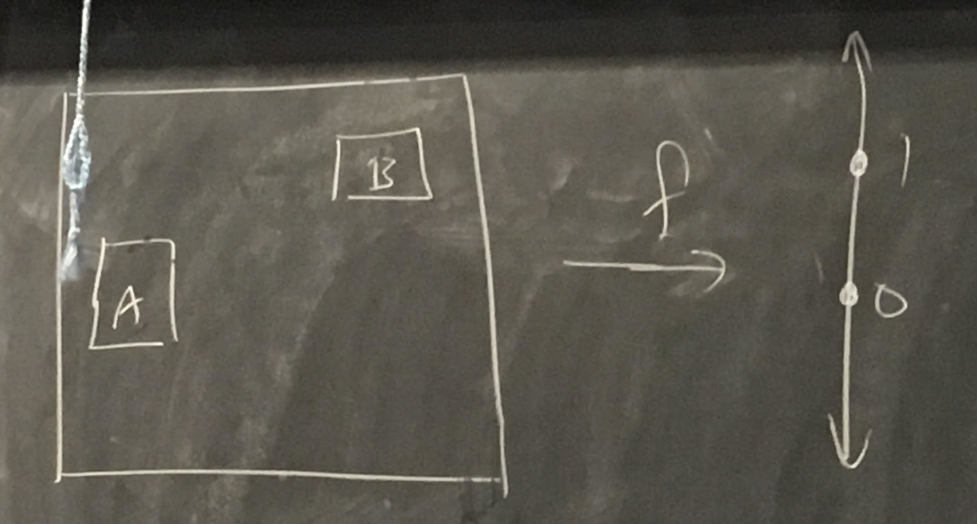
\includegraphics[scale=.18]{images/separation_4}
\end{center}

\begin{remark*}\mbox{}
\begin{enumerate}
\item This property characterizes normal spaces, i.e. if $X$ is a space that has this property for all disjoint closed pairs of sets, then $X$ is normal. 
\item In a statement of Urysohn's Lemma, we can replace $[0,1]$ with any closed interval. 
\end{enumerate}
\end{remark*}

\begin{proof}
Ennumerate the rational numbers in $[0,1]$ as $0,1,r_1, r_2, \ldots$. By Prop 37, there is an open set $U_0$ with $A \subset U_0 \subset \closure{U_0} \subset X-B$. 

\begin{center}
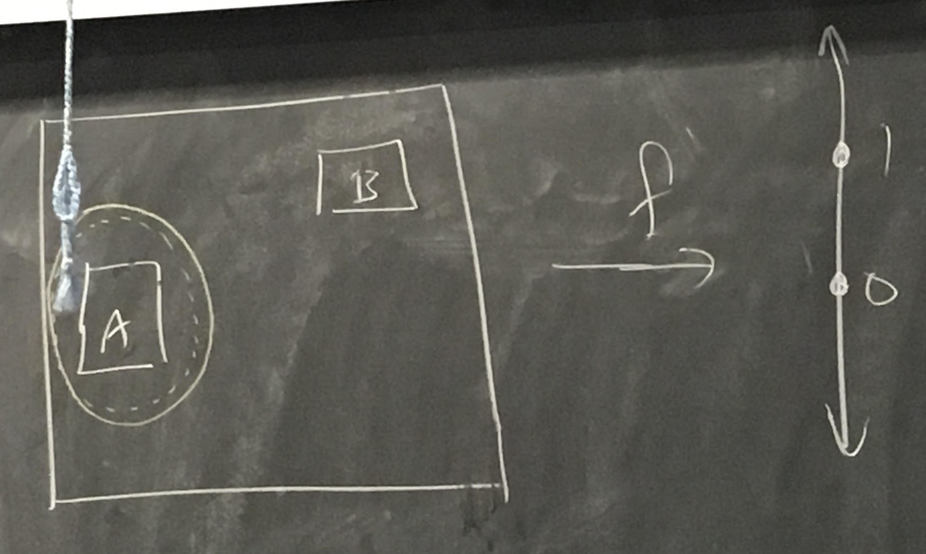
\includegraphics[scale=.18]{images/separation_5}
\end{center}

Let $U_1=X-B$. Now, we can select $U_{r_1}$ with 
$$U_0 \subset U_{r_1} \subset \closure{U_{r_1}} \subset U_1.$$
Inductively, suppose we have defined $U_{r_1}, \ldots U_{r_n}$ such that $r_i<r_j$ implies $\closure{U_{r_i}}\subset U_{r_j}$. Given $r_{n+1}$, we have that $r_j<r_{n+1}<r_k$, for some $1\leq j,k \leq n$ and all other $r_i$ have either $r_i<r_j$ or $r_i>r_k$; OR
$0<r_{n+1}<r_i$ for all $i\in \N$, OR $r_i<r_{n+1}<1$ for all $i\in \N$. In any case, use Prop 37 to find and open set $U_{r_{n+1}}$ with 
$$\closure{U_{r_j}}\subset U_{r_{n+1}} \subset \closure{U_{r_{n+1}}} \subset U_k.$$

\begin{center}
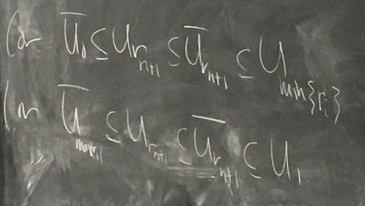
\includegraphics[scale=.35]{images/separation_6}
\end{center}

Basically, we have constructed a collection of nested open sets, such that the nesting has the same ordering as the rationals. Again, we have a collection of open sets $U_r, r\in \Q$, with $A\subset U_0$ and $p<q$ implies $\closure{U_p} \subset U_q$. 

$$\text{Let } f(x)=\inf\{r:x\in U_r\}.$$
\end{proof}

\begin{highlight}
\begin{theorem}[Tietze's Extension Theorem] Let $X$ be normal, with $A$ being closed in $X$, and let $f:A\to \R$ be a continuous function. Then there exists $F:X\to \R$ with $F(a)=f(a)$ for all $a\in A$. 
\end{theorem}
\end{highlight}

\begin{remark*}
The proof follows from Urysohn's Lemma, and also in the homework, we prove that Urysohn's Lemma follows from Tietze's Extension Theorem. There exist proofs of Tietze's Extension Theorem which do not rely on Urysohn's Lemma, so the two statements are equivalent. 
\end{remark*}

\section{Connectedness}

\begin{highlight}
\begin{definition*}
A space $X$ is \emph{connected} if it is not the union of two non-empty disjoint sets. 
\end{definition*}
\end{highlight}
Specifically, this means $X$ is connected if whenever $X=U\cup V$ with $V,U$ open and $U\cap V=\emptyset$, we must have $U=\emptyset$ or $V=\emptyset$. 

\begin{definition*}
If $X$ is not conected, we say $U\cup V=X$ with $U,V$ non-empty disjoint sets is a \emph{separation} of $X$. 
\end{definition*}

\begin{highlight}
\begin{theorem}[Characterization of a Connected Space]\mbox{}\\
The following are equivalent:
\begin{enumerate}[label=(\roman*)]
\item $X$ is not the union of two non-empty disjoint open sets. 
\item $X$ is not the union of two non-empty disjoint closed sets. 
\item The only sets in $X$ which are both open and closed are $\emptyset$ and $X$. 
\item There is no continuous onto function $f:X\to \{0,1\}$, where $\{0,1\}$ has the discrete topology. 
\end{enumerate}
\end{theorem}
\end{highlight}

\begin{proof}[(i)$\implies$(ii)]
Suppose $X=C\cup D$, with $C,D$ closed and disjoint. Now, this means that $C=(X-D)$ and $D=(X-C)$, so $X=(X-C)\cup (X-D)$, where $(X-C),(X-D)$ are both open and disjoint. Now, since $X$ is connected, then either $(X-C)=\emptyset$ or $(X-D)=\emptyset$, thus either $C=\emptyset$ or $D=\emptyset$. 
\end{proof}

\begin{proof}[(ii)$\implies$(iii)]
Suppose $C$ is both open and closed. Now obviously, $X=(X-C)\cup C$, for any $C$. Since $C$ is both open and closed, then $(X-C)$ is closed and $C$ is closed. So by (ii), either $X-C=\emptyset$ or $C=\emptyset$. 
\end{proof}

\begin{proof}[(iii)$\implies$(iv)]
Suppose $f:X\to \{0,1\}$ is continuous. Note that $\{0\},\{1\}$ are both open and closed. Consider $\preimage{f}{\{0\}}$. Since $f$ is continuous,$\preimage{f}{\{0\}}$ is closed and open. So by (iii), $\preimage{f}{\{0\}}$ is either $X$ or $\emptyset$. This means either $f\equiv0$ or $f\equiv1$, so it is not onto. \end{proof}

\begin{proof}[(iv)$\implies$(i)] (Proof by contrapositive)
Suppose $X=U\cup V $ is a separation of $X$. Define $f:X\to \{0,1\}$ as follows:
$$f(x)=
\begin{cases}
0 & x\in U\\
1 & x\in V\\
\end{cases}
$$
Now clearly, $f$ is both continuous and onto. (If you're not convinced, consider the preimage of each open set in $\{0,1\}$. There are only four of them.)
\end{proof}

\begin{highlight}
\begin{theorem}\mbox{}
\begin{enumerate}[label=(\roman*)]
\item $\R$ is connected. 
\item $\Q$ is not connected. 
\end{enumerate}
\end{theorem}
\end{highlight}
\begin{proof}(i)
Suppose for contradiction that $\R= A\cup B$, with $A,B$ closed, disjoint, and nonempty.\\
 Pick $a_0\in A$, $b_0\in B$, and without loss of generality, assume that $a_0<b_0$. Let $$S_{b_0}=\{a\in A: a<b_0\}.$$ Now, $a_0\in S_{b_0}$, so $S_{b_0}$ is nonempty and bounded above. So there exists $\alpha=\sup{S_{b_0}}$. Since $\alpha=\sup{S_{b_0}}\in \closure{A}$ and $A$ is closed, then $\alpha\in A$. By our definition of $S_{b_0}$, we have that $(\alpha, b_0)\not\subset A$, so it must be a subset of $B$. Since $(\alpha, b_0)\subset B$ and $B$ is closed, then $\alpha \in B$. Thus, $\alpha\in A\cap B$, which contradicts our assumption that $A$ and $B$ are disjoint. 
\end{proof}
\begin{proof}(ii)
To see that $\Q$ (as a subspace of $\R$) is not connected, let 
$$U=\left((-\infty, \pi)\cap\Q\right),$$
$$V=\left((\pi, \infty)\cap\Q\right).$$
Now observe that $\Q=U\cup V$, and $U$ and $V$ are disjoint open sets in $\Q$. Thus, we have produced a separation of $\Q$, so it is not connected. 
\end{proof}

\subsection{Properties of Connected Sets}
\begin{highlight}
\begin{proposition}
Suppose $C$ is a connected subset of $X$, and we have ${C\subset U \cup V}$, with $U,V$ being open and disjoint. 

Then, $C\subset U$ or $C\subset V$. 
\end{proposition}
\end{highlight}
\begin{proof}
(to be added soon)
\end{proof}

\begin{highlight}
\begin{theorem}
Suppose $A$ is a connected subset of $X$, and $B$ is a subset $A\subset B\subset \closure{A}$. 

Then $B$ is connected. In particular, $A$ connected implies $\closure{A}$ is connected. 
\end{theorem}
\end{highlight}
\begin{proof}
(homework exercise)
\end{proof}

\begin{highlight}
\begin{theorem}
Suppose $f:X\to Y$ is a continuous function, and $X$ is connected.

Then, $f(X)$ is connected. In particular, if $f$ is onto, then $Y$ is connected. 
\end{theorem}
\end{highlight}
\begin{proof}
Suppose for contradiction that $f(X)$ is not connected. Then $f(X)=V\cup W$, for some sets $V,W$ which are nonempty, disjoint, and open in $Y$. This means that $X=\preimage{f}{V}\cup \preimage{f}{W}$, with $\preimage{f}{V}, \preimage{f}{W}$ being nonempty, disjoint, and open in $X$. Thus, we have a separation of $X$, which contradicts our assumption that $X$ is connected. 
\end{proof}

\begin{highlight}
\begin{theorem}
Suppose that $\arbcoll{A}$ is a collection of connected subsets of a space $X$, and $p\in A_\alpha$ for all $\alpha\in\Gamma$. Then, $\arbcup{A}$ is connected. 
\end{theorem}
\end{highlight}
\begin{proof}
Suppose $\arbcup{A}=U\cup V$ with $U\cap V=\emptyset$. For each $\alpha$, we have $A_\alpha\in U\cup V$, so by Proposition 42, $A_\alpha \subset U$ or $A_\alpha \subset V$. But if $p\in U$, then we have $A_\alpha \subset U$ for all $\alpha \in \Gamma$. So $\arbcup{A}\subset U$, and $V=\emptyset$. 
\end{proof}

\begin{highlight}
\begin{definition*}
Let $X$ be a space, with $p\in X$. The \emph{connected component of $p\in X$}, denoted $C_p$, is 
$$\bigcup_{p\in k,  k \text{connected}} k.$$
\end{definition*}
\end{highlight}
Observe that by Thm 45, $C_p$ is connected. Furthermore, $C_p$ is closed. This follows from Thm 43, since $\closure{C_p}$ is then connected, and so $\closure{C_p}\subset C_p$. 

\begin{highlight}
\begin{theorem}
Let $X,Y$ be spaces. $A\times Y$ is connected if and only if $X$ and $Y$ are connected. 
\end{theorem}
\end{highlight}
\begin{proof}[$\implies$]
If $X\times	Y$ is connected, then $\Pi_x(X\times Y)=X$ and $\Pi_y(X\times Y)=Y$ are connected by Thm 44. 
\end{proof}
\begin{proof}[$\impliedby$]
Suppose $X$ and $Y$ are both connected. Let $(x_0, y_0)\in X\times Y$. Let $(x,y)$ be and arbitrary element of $X\times Y$. 
[image]
Now, $(X\times \{y\})\cup (\{x_0\}\times Y)$ is the union of connected subsets with $(x_0,y)$ in common, so it is connected. Thus, $(x,y)\in C_{(x_0,y_0)}$. Since $(x,y)$ was arbitrarily chosen, this gives $C_{(x_0,y_0)}=X\times Y$. 
\end{proof}
\begin{example*}
This shows that $\R^n$ is connected. 
\end{example*}

\subsection{Path Connectedness}

\begin{highlight}
\begin{definition*}
Let $X$ be a space. A \emph{path (in X)} is a continuous function $f:[0,1]\to X$. 
\end{definition*}
\end{highlight}

\begin{highlight}
\begin{definition*}
A space $X$ is \emph{path-connected} if for every $x,y\in X$, there is a path $f:[0,1]\to X$ with $f(0)=x$ and $f(1)=y$. 
\end{definition*}
\end{highlight}

\begin{highlight}
\begin{theorem}
If $X$ is path-connected and $g:X\to Y$ is continuous, then $g(X)$ is path-connected. 
\end{theorem}
\end{highlight}
\begin{proof}\mbox{}
$$\text{[image]}$$
Let $y_1, y_2 \in g(X)$. There are $x_1, x_2\in X$ with $g(x_1)=y_1, g(x_2)=y_2$. Since $X$ is path-connected, there is some $f:[0,1]\to X$ with $f(0)=x_1$ and $f(1)=x_2$. Then, $g\circ f:I\to g(X)$ is a path such that $0 \mapsto y_1$ and $1 \mapsto y_2$. 
\end{proof}

\begin{example*}
$$\text{[image]}$$

$$\text{[image]}$$

$$\text{[image]}$$
\end{example*}

\begin{highlight}
\begin{theorem}
If $X$ is path-connected, then $X$ is connected. 
\end{theorem}
\end{highlight}
\begin{proof}
Let $x_0\in X$, and let $x\in X$ be arbitrary. 

$$\text{[image]}$$

Since $X$ is path-connected, then there exists $f_X:[0,1]\to X$ with $f(0)=x_0, f(1)=x$. this gives us that 
$$X=\bigcup_{x\in X} f_x([0,1]),$$
which is connected by Thm 45. (Note: each $f_x([0,1])$) is connected and contains $x_0$.)
\end{proof}

\begin{highlight}
\begin{remark*}
The converse of Theorem 48 is false. 
\end{remark*}
\end{highlight}
\begin{example*}
$$\text{[image]}$$

\textit{Claim:} $A$ is not path-connected. \\
Suppose for contradiction that there is a path $f:[0,1]\to A$ with $f(0)=x_0\in A_0, f(1)=x_1\in A_1$. Note that $A_0$ is closed in $A$, so $\preimage{f}{A_0}$ is closed in $[0,1]$. 

\textit{Subclaim:} $\preimage{f}{A_0}$ is open in $A$. (If this is the case, then $A_0$ is both open and closed.) \\
Let $t\in\preimage{f}{A_0}$. Let $B=B(f(t), \sfrac{1}{4})$, and consider $A\cap B$.

$$\text{[image]}$$

$$\text{[image]}$$

Observe that the connected component of $f(t)$ in $A\cap B$ is $A_0\cap B$. Note $t\in \preimage{f}{A\cap B}$ is open, so there exists $\epsilon>0$ such that $(t-\epsilon, t+\epsilon)\subset\preimage{f}{A\cap B}$. So $f(t-\epsilon, t+\epsilon)\subset A\cap B$. But $f(t-\epsilon, t+\epsilon)$ is connected, so in fact, 
$$f(t-\epsilon, t+\epsilon)\subset A_0\cap B \subset A_0.$$
So $(t-\epsilon, t+\epsilon)\subset \preimage{f}{A_0}$. This shows $\preimage{f}{A_0}$ is open. \qedwhite \\
Now, we have shown that $\preimage{f}{A_0}$ is both open and closed. Since $\preimage{f}{x_0}\in \preimage{f}{A_0}$ so it is non-empty, and $\preimage{f}{A_0}\neq [0,1]$ because $\preimage{f}{x_1}\not\in \preimage{f}{A_0}$. \qed
\end{example*}

\begin{highlight}
\begin{theorem}
If $W$ be a connected open subset of $\R^n_{usual}$, then $W$ is path-connected. 
\end{theorem}
\end{highlight}
\begin{proof}
Let $x_0\in W$. Let\\
$U=\{x\in W:$ There is a path in $W$ from $x_0$ to $x\}$\\
$V=\{x\in W:$ There is NOT a path in $W$ from $x_0$ to $x\}$\\
with $W=U\cup V, U\cap V=\emptyset$. 

\begin{center}
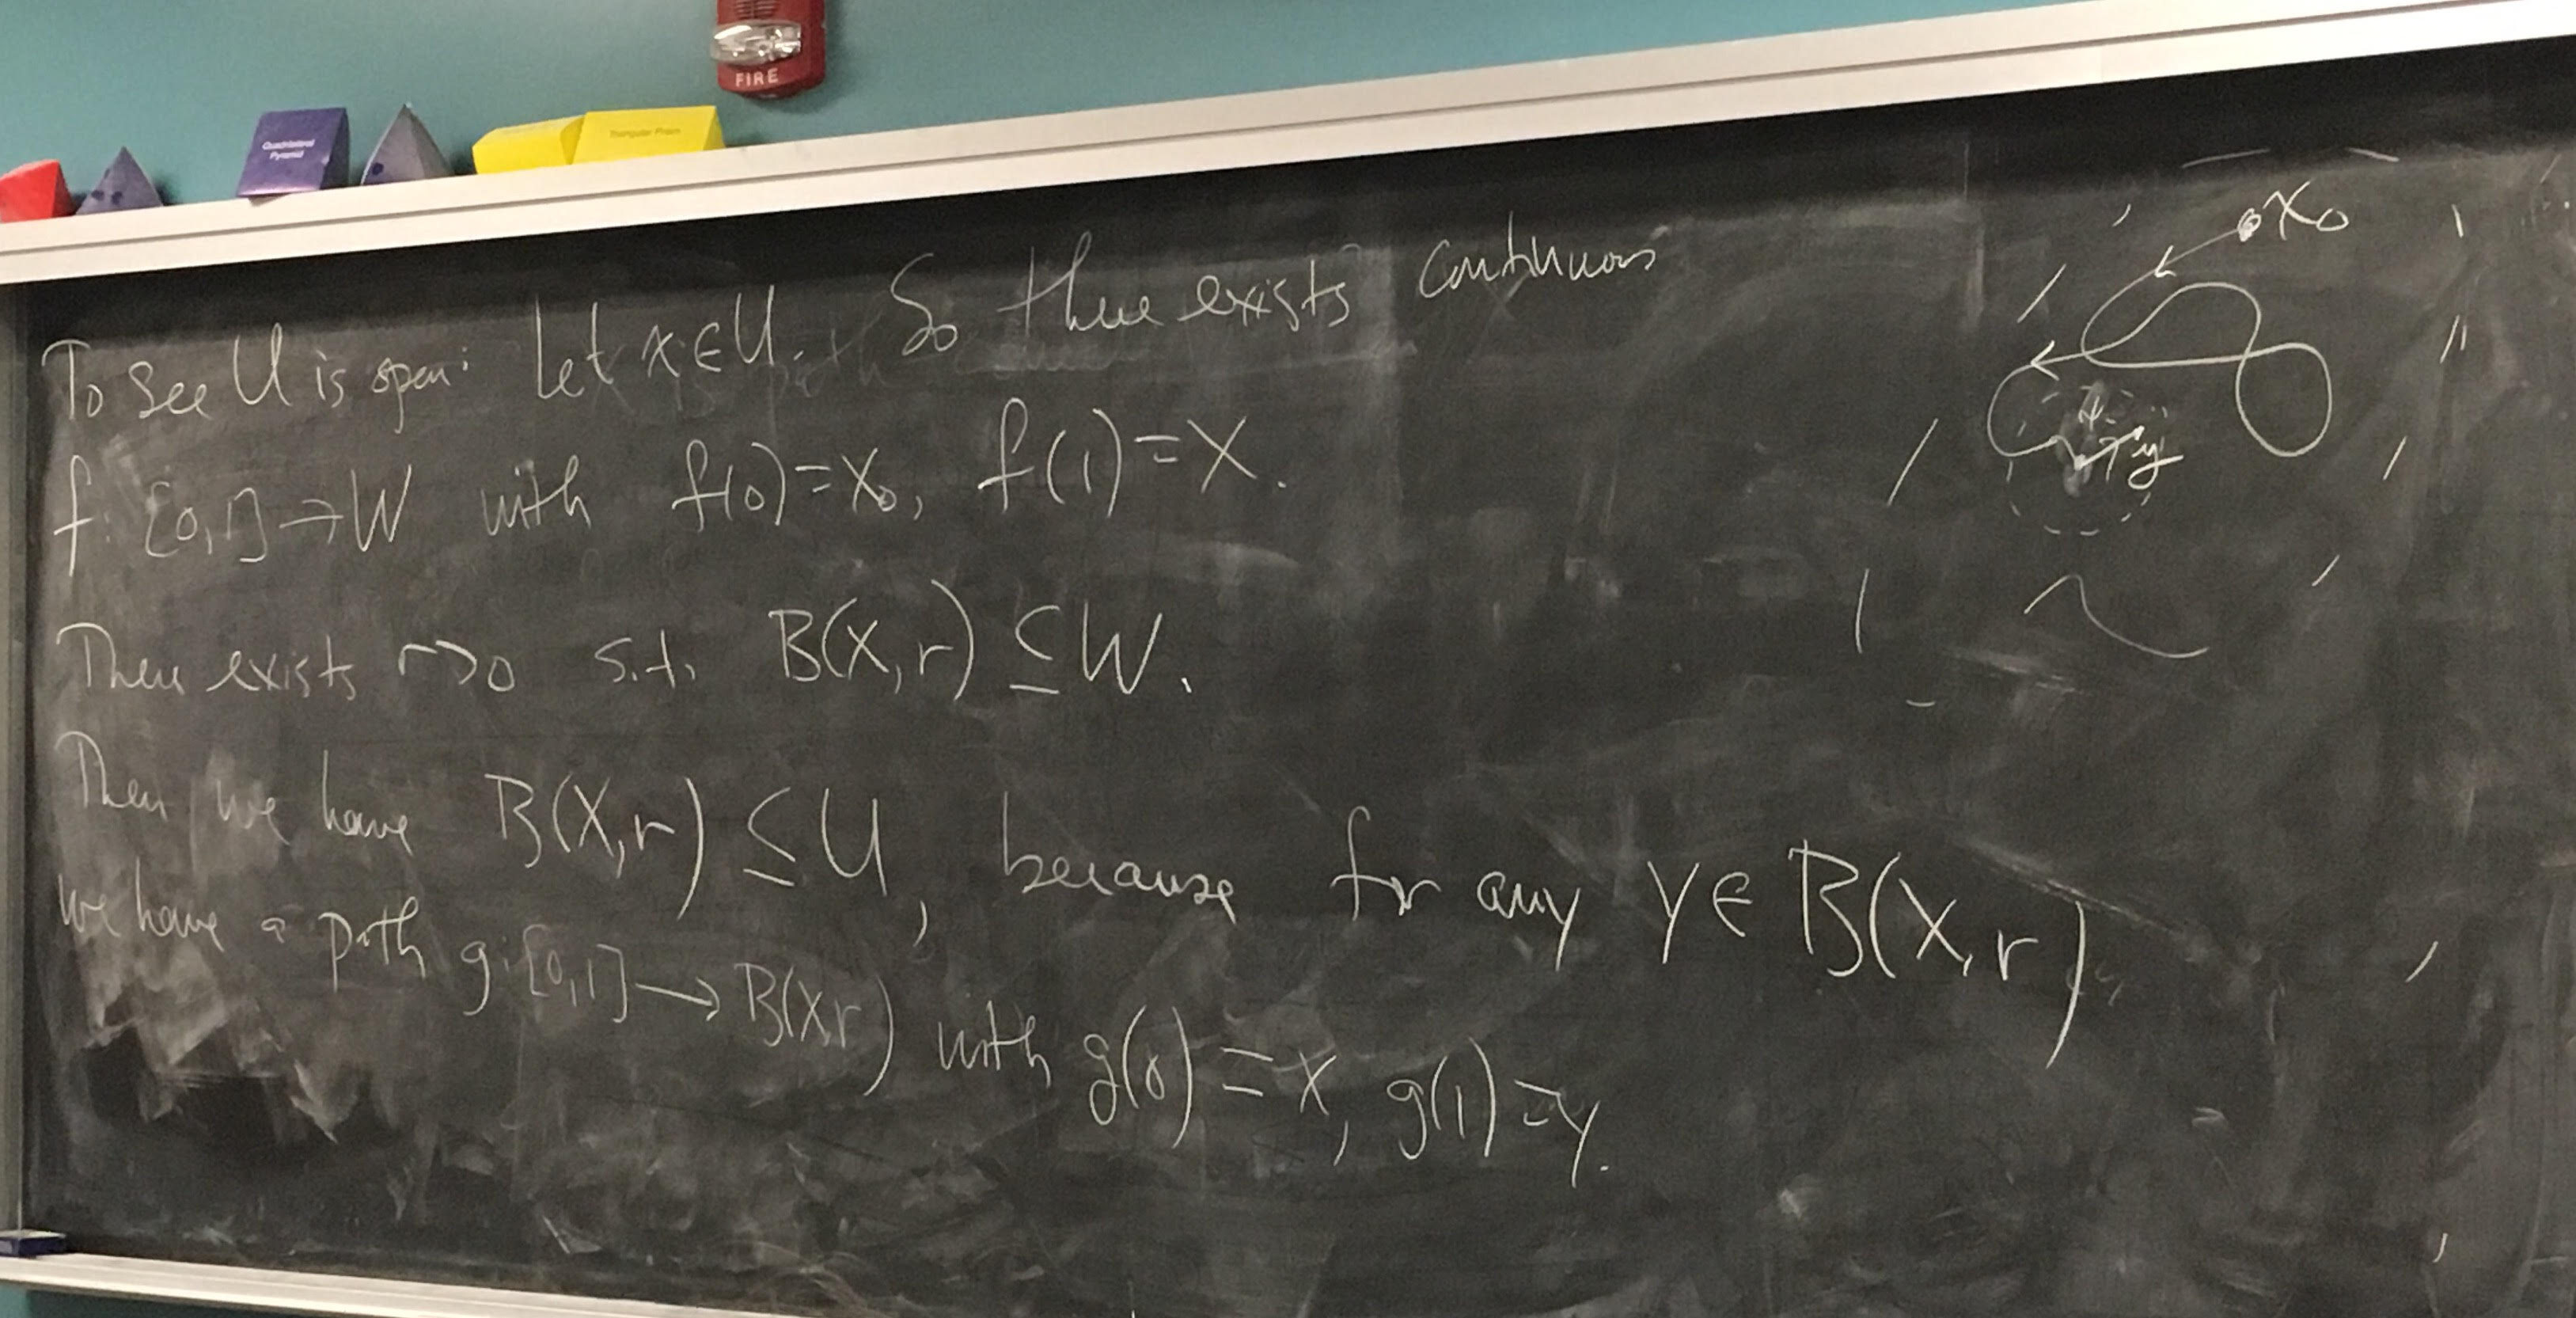
\includegraphics[scale=.08]{images/path_connectedness1}
\end{center}

So, we can concatenate these paths to get a path (sometimes called $f\dot g$)  $f\dot g: [0,1]\to W$
$$(f\dot g)(t) = 
\begin{cases}
f(2t) & 0\leq t\leq \frac{1}{2}\\
g(2t-1) & \frac{1}{2}\leq t\leq 1\\
\end{cases}_.$$
Then, $y\in U$. We have $x\in B(x,r)\subset U$, so $U$ is open. 

To see that $V$ is open: Let $x\in V$. So there does not exist any path from $x_0$ to $x$. Since $W$ is open, there is $r>0$ such that $B(x,r)\subset W$. In fact, $B(x,r)\subset V$, because if $y\in B(x,r)$, then there is a path $h:[0,1]\to B(x,r)$ with $h(0)=$ some $y$ and $h(1)=x$. If $y\in U$, there would be a path $k:[0,1]\to W$ from $x_0$ to $y$. But then the concatenated path $kh$ (defined as before) connects $x_0$ and $x$, which contradicts $x\in V$. So in fact, $y\in V$, and we have $B(x,r)\subset V$, showing $V$ is open. 

Now, $W=U\cup V$ with $U,V$ both being open and disjoint, and $U$ being nonempty (since $x_0\in U$). Since $W$ is connected, then $V$ is empty, and $W=U$. 

\end{proof}

\pagebreak
\section{Product Spaces in General}
\subsection{Motivation}

Recall: 
\begin{itemize}
\item If $X,Y$ are spaces, $X\times Y = \{(x,y):x\in X, y\in Y\}$ has the \emph{product topology} defined with basis sets of the form $U\times V$, where $U$ open in $X,$ and $V$ open in $Y$. 

\item Similarly, this generalizes to, given $X_1, \ldots X_n$ spaces, 
$$X_1 \times \ldots \times X_n = \{(x_1, \ldots, x_n)\}$$
has product topology defined as you would expect.


\item You already know of some general product spaces:
$$\R^n = \R \times \R \times \ldots \R = \{(x_1, \ldots, x_n): x_i\in\R \}$$
You can think of this as a sequence or, more formally, a function $a: \{1,2,3, \ldots n\} \to \R$, (or whatever your space is), where $a(n)$ is the $n$-th term of the sequence.  
\end{itemize} 

\subsection{Definition of Arbitrary Product Spaces}

\begin{highlight}
\begin{definition*}
Let $\arbcoll{X}$ be a collection of sets. 
$$\arbprod{X} = \{f:\Gamma \to \arbcup{X} | f(\alpha)\in X_\alpha\}$$
Given some $f\in\arbprod{X}$, we refer to $f(\alpha)$ as the $\alpha$-th coordinate of $f$, and we sometimes write $f=\arbcoll{f}$, where $f_\alpha=f(\alpha)$. 
\end{definition*}
\end{highlight}

\begin{highlight}
\begin{definition*}
We define $\pi_\beta : \arbprod{X}\to X_\beta$ by $\pi_\beta(f)=f(\beta)$, for any $\beta\in\Gamma$. 

This is called \emph{projection onto $X_\beta$.}
\end{definition*}
\end{highlight}

\begin{example*}
Let $\Gamma=\{1,2,\ldots, n\}$.\\
Let $\R_1, \R_2, \ldots, \R_n$ be $n$ copies of $\R$. 
$$\prod_{i\in\N} \R_i = \R^n. $$
\end{example*}

\begin{center}
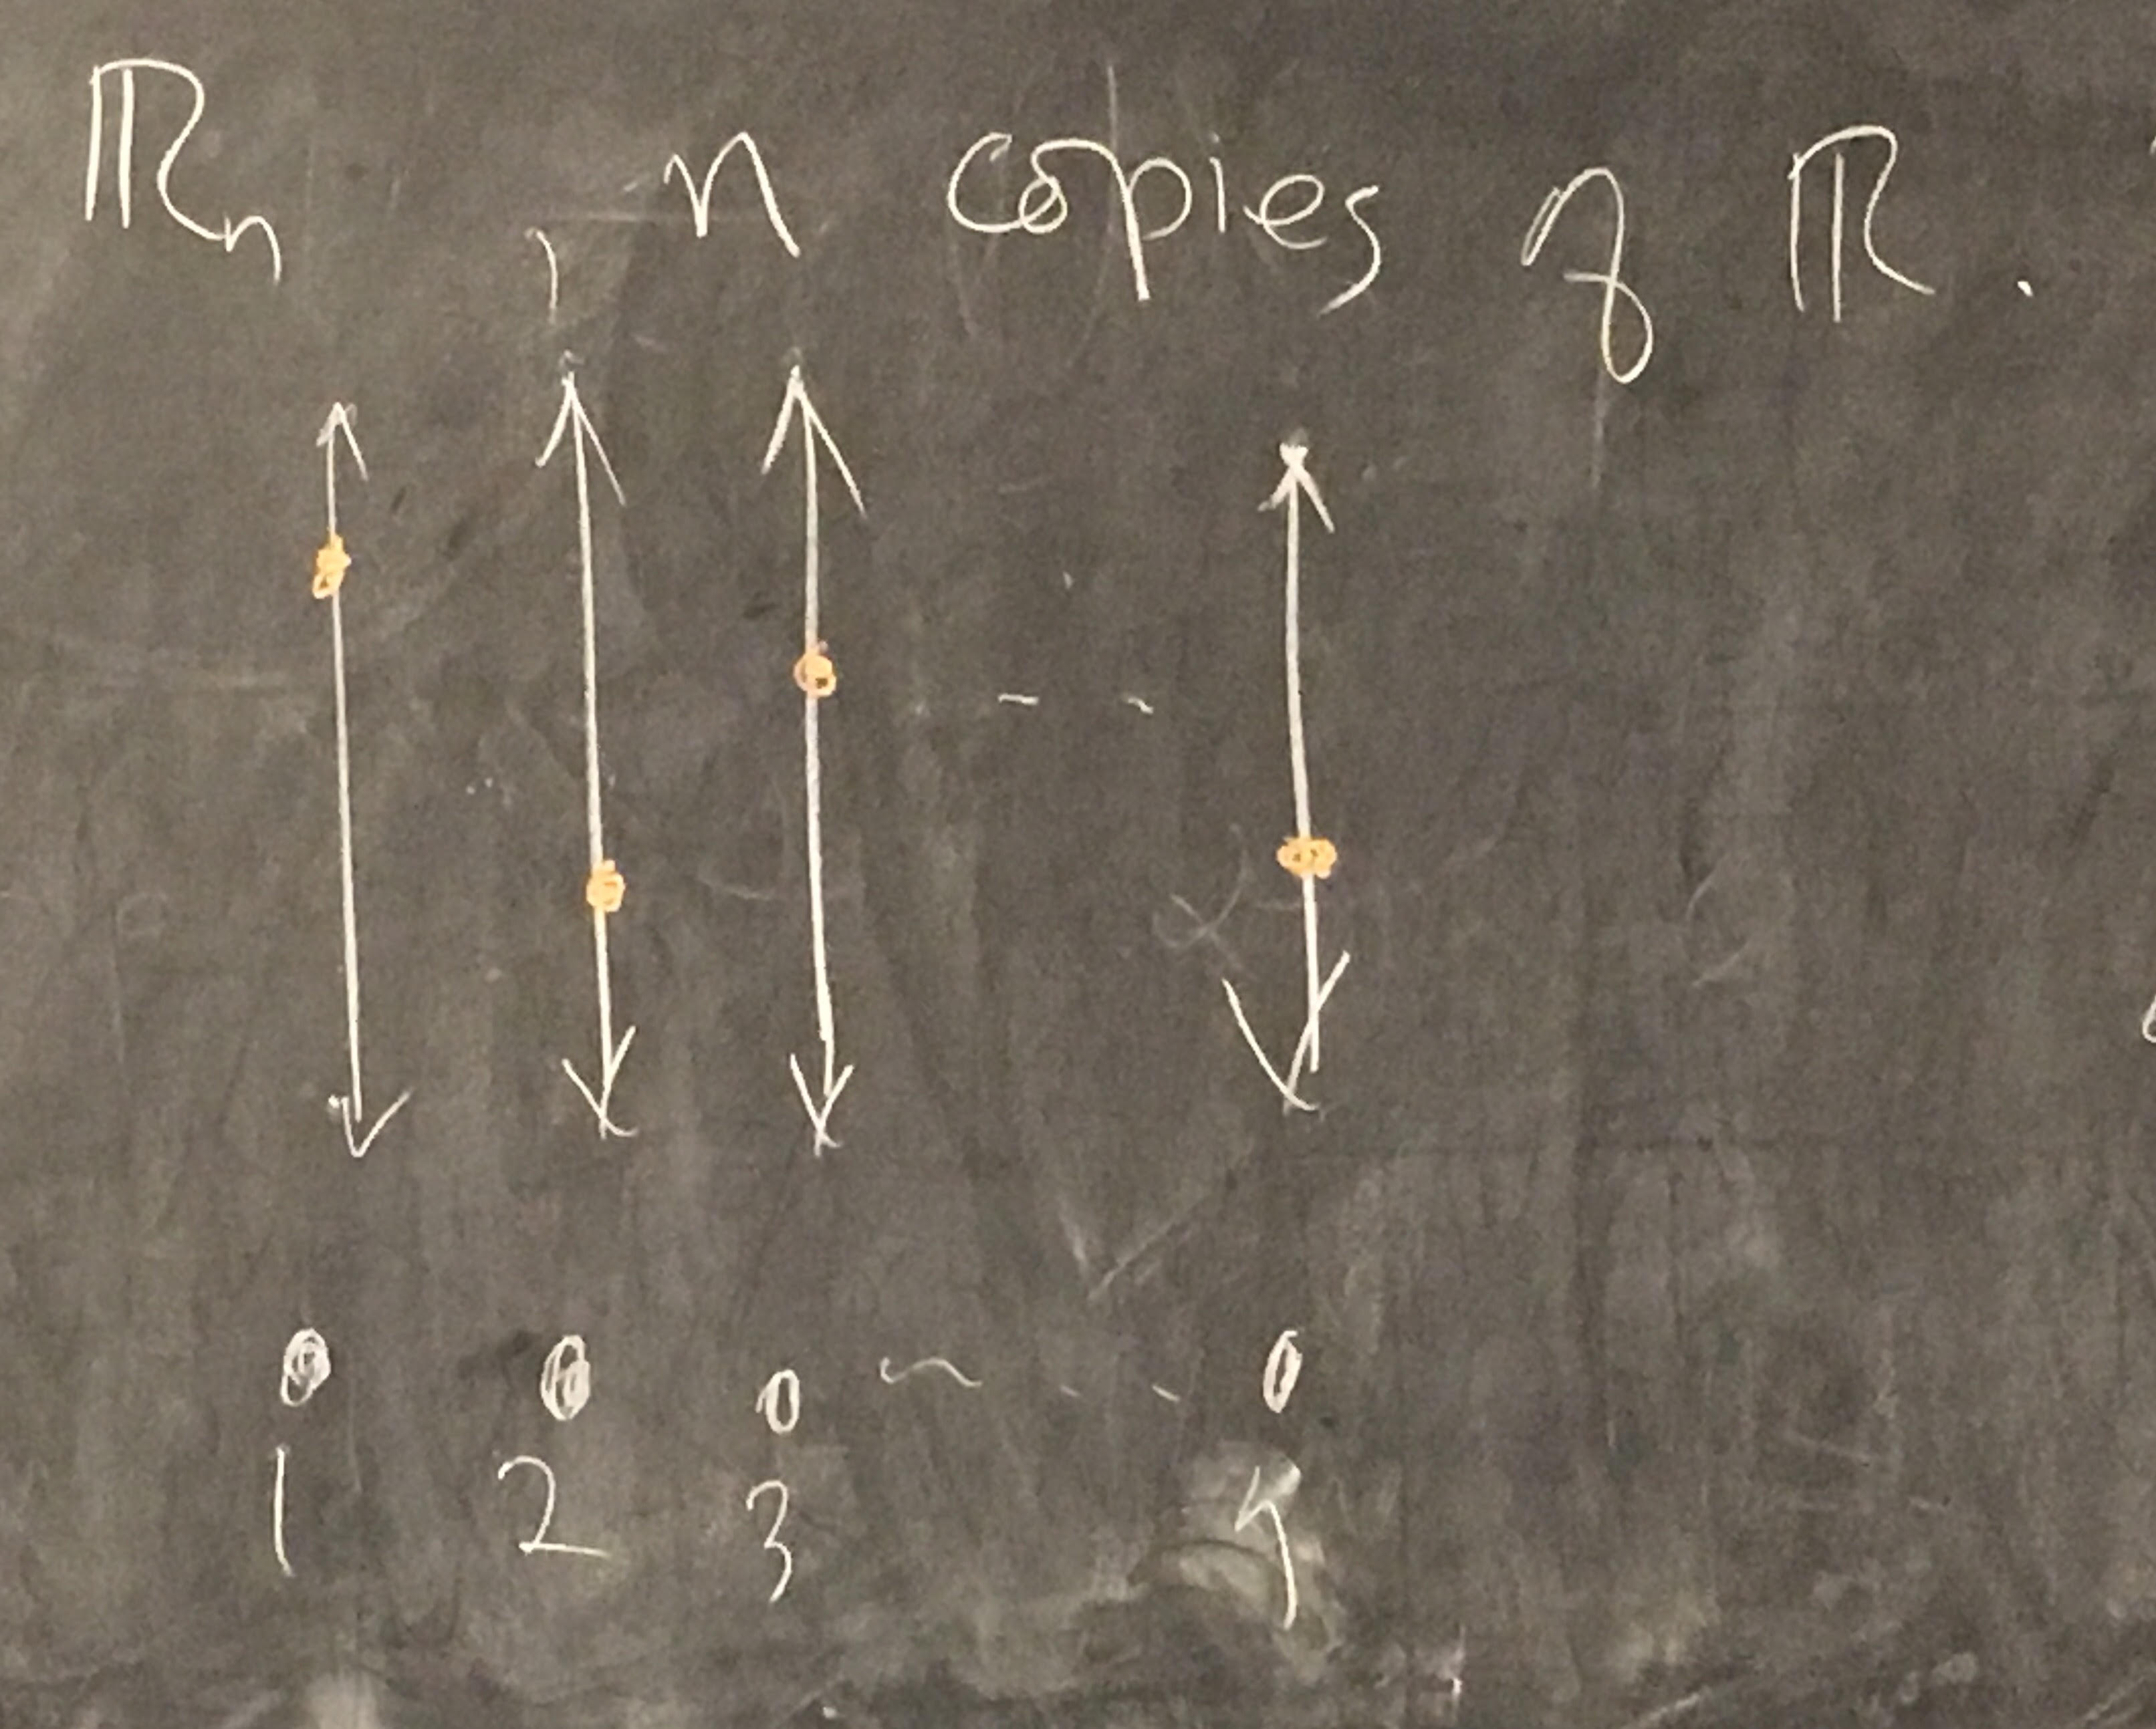
\includegraphics[scale=.04]{images/general_products3}
\end{center}

In general, a vector looks like this:
\begin{center}
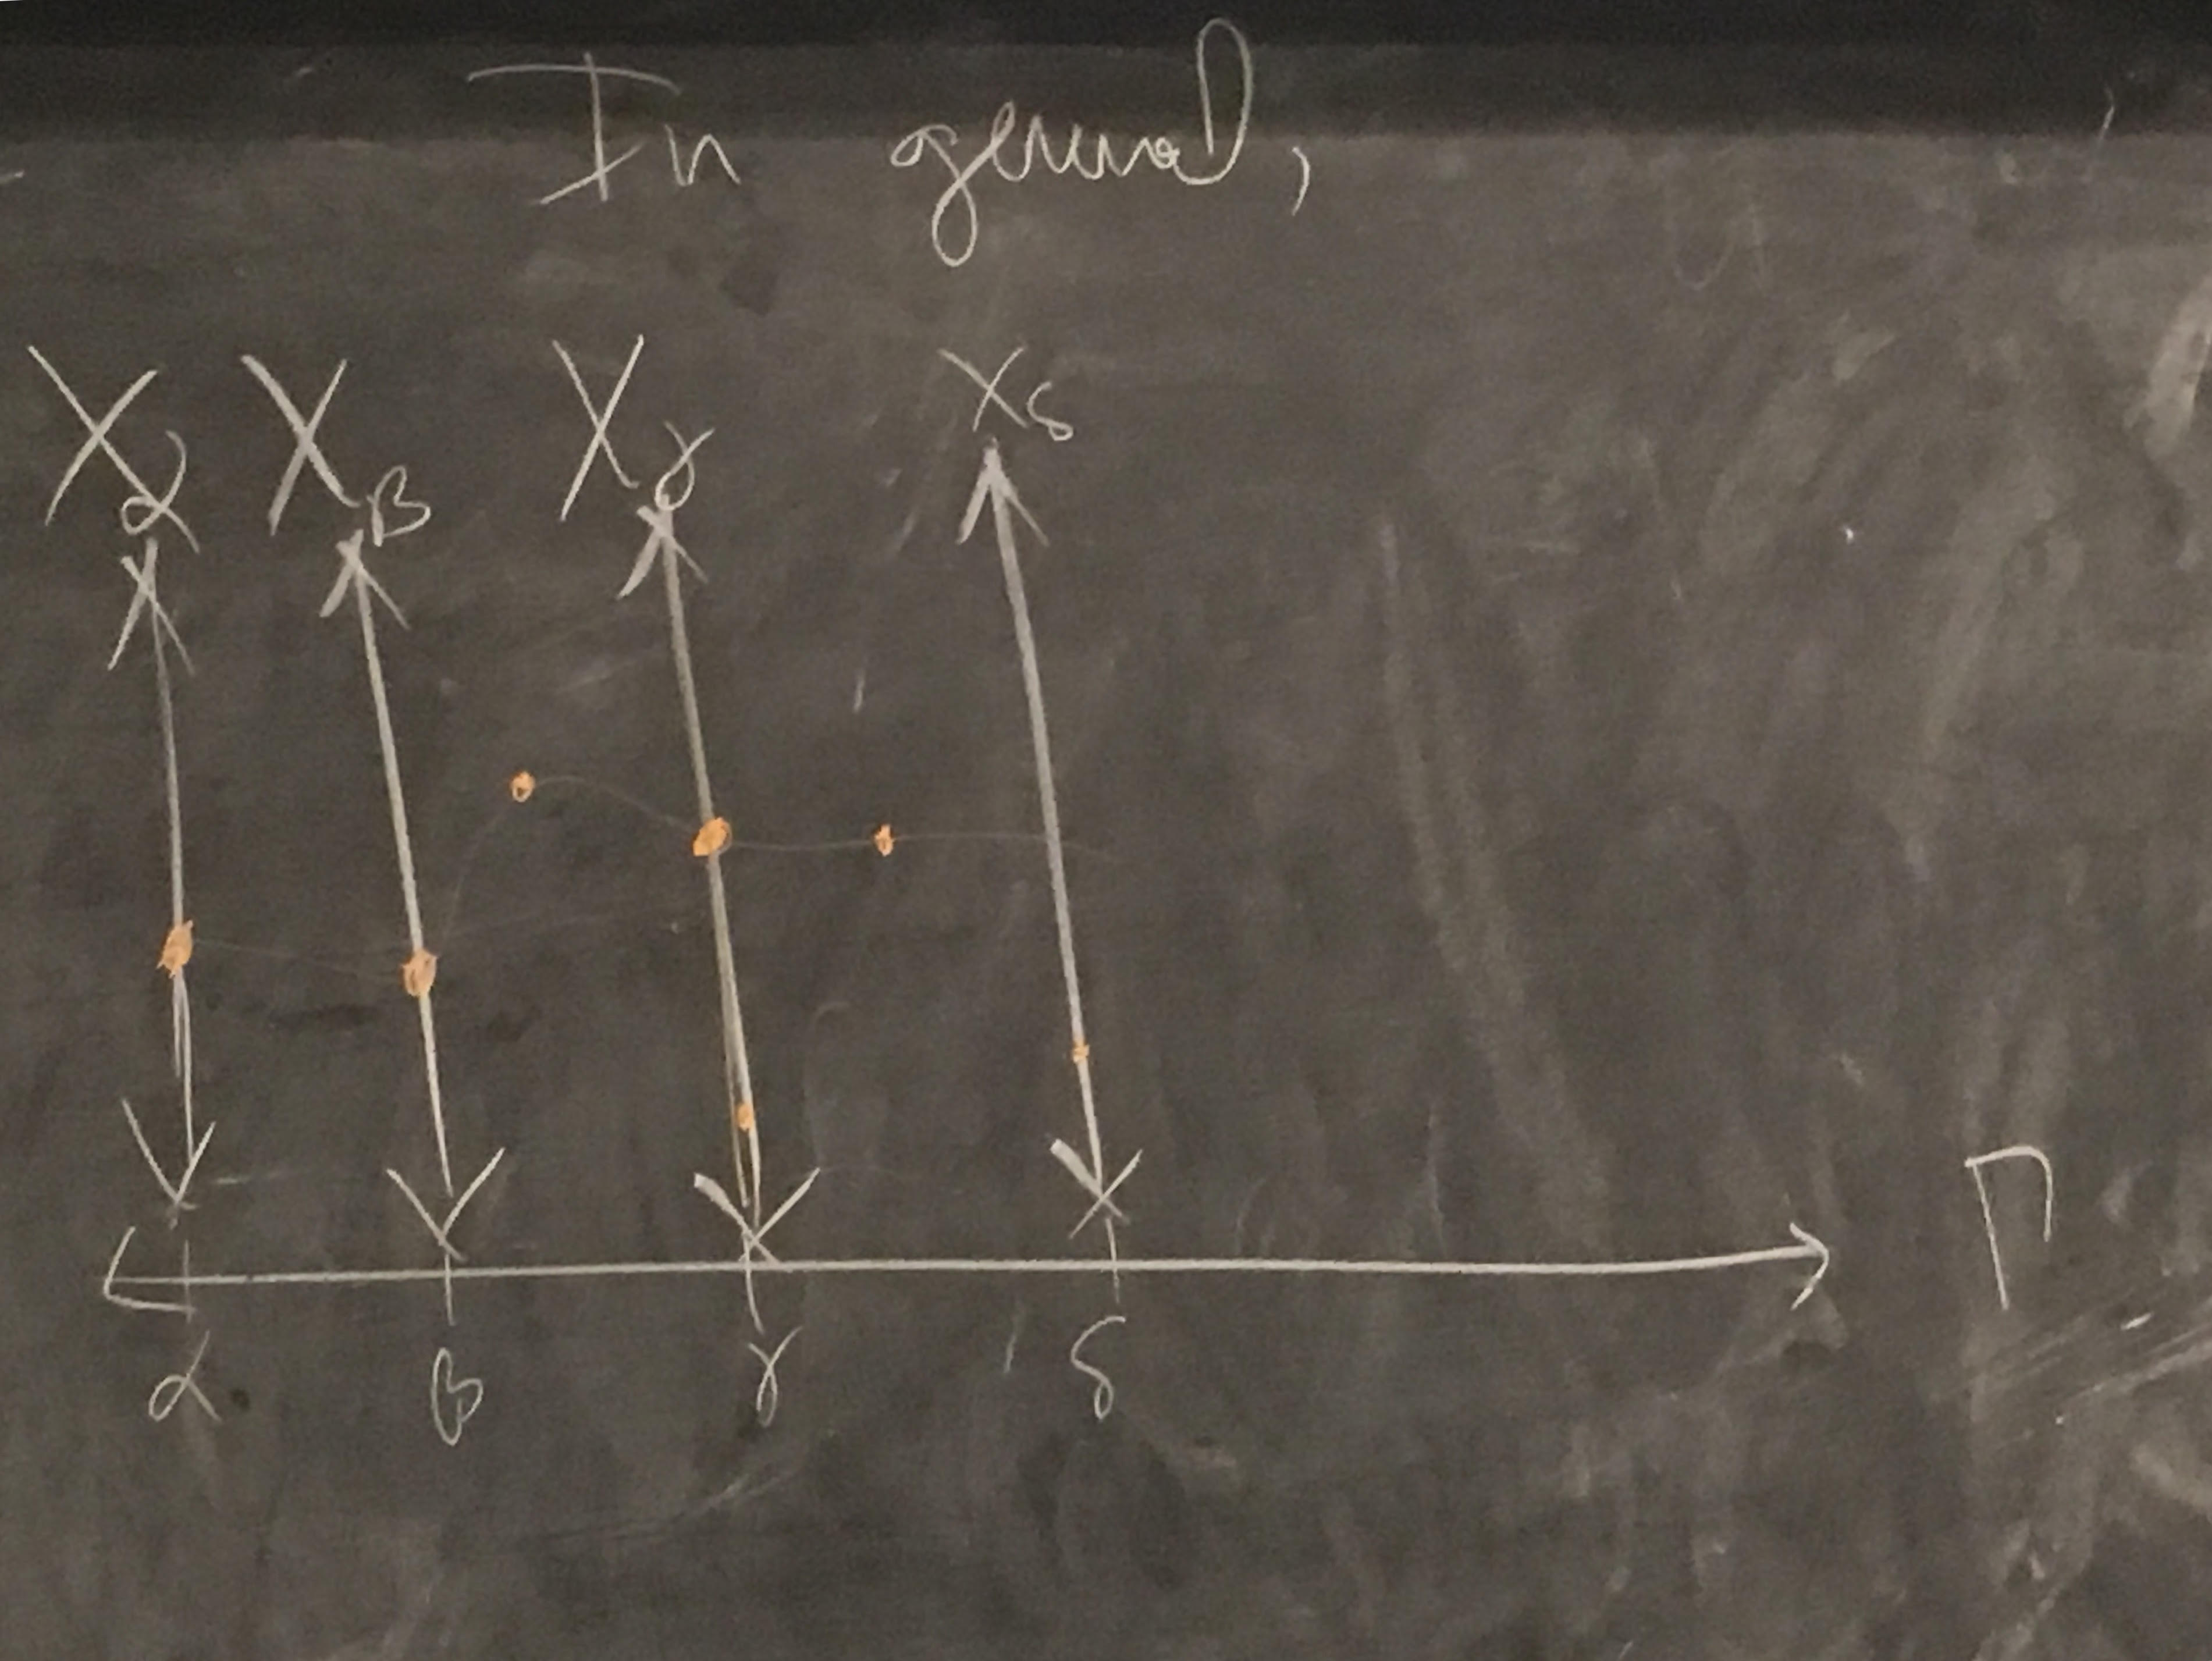
\includegraphics[scale=.04]{images/general_products4}
\end{center}

\begin{highlight}
\begin{definition*}
Given $\arbcoll{X}$ topological spaces, the collection of all $\pi^{-1}_\beta(U_\beta)$ for all open sets $U_\beta\in X_\beta$ and all $\beta\in\Gamma$, forms a subbasis for a topology on $\arbprod{X}$. This is called the \emph{product topology on $\arbprod{X}$}.
\end{definition*}
\end{highlight}
\begin{highlight}
That is, a basic sets in the product topology are of the form 
$$\arbprod{U}, \text{where each } U_\alpha\subset X_\alpha \text{is open and } U_\alpha=X_\alpha \text{ except finitely many } \alpha \text{s.}$$
\end{highlight}

\begin{example*}[1]\mbox{}\\
$\Gamma = [n] = \{1,2,\ldots, n\}$\\
$\arbprod{\R}=R^n$. 

If $U$ is open in $\R$, then 
$$\preimage{\Pi_1}{U}=\overbrace{U\times\R\times \ldots \R}^{n \text{ of these}}$$
\end{example*}

\begin{example*}[Another number 1]
Consider $X_1\times X_2$, $\Gamma=\{1,2\}$

\begin{center}
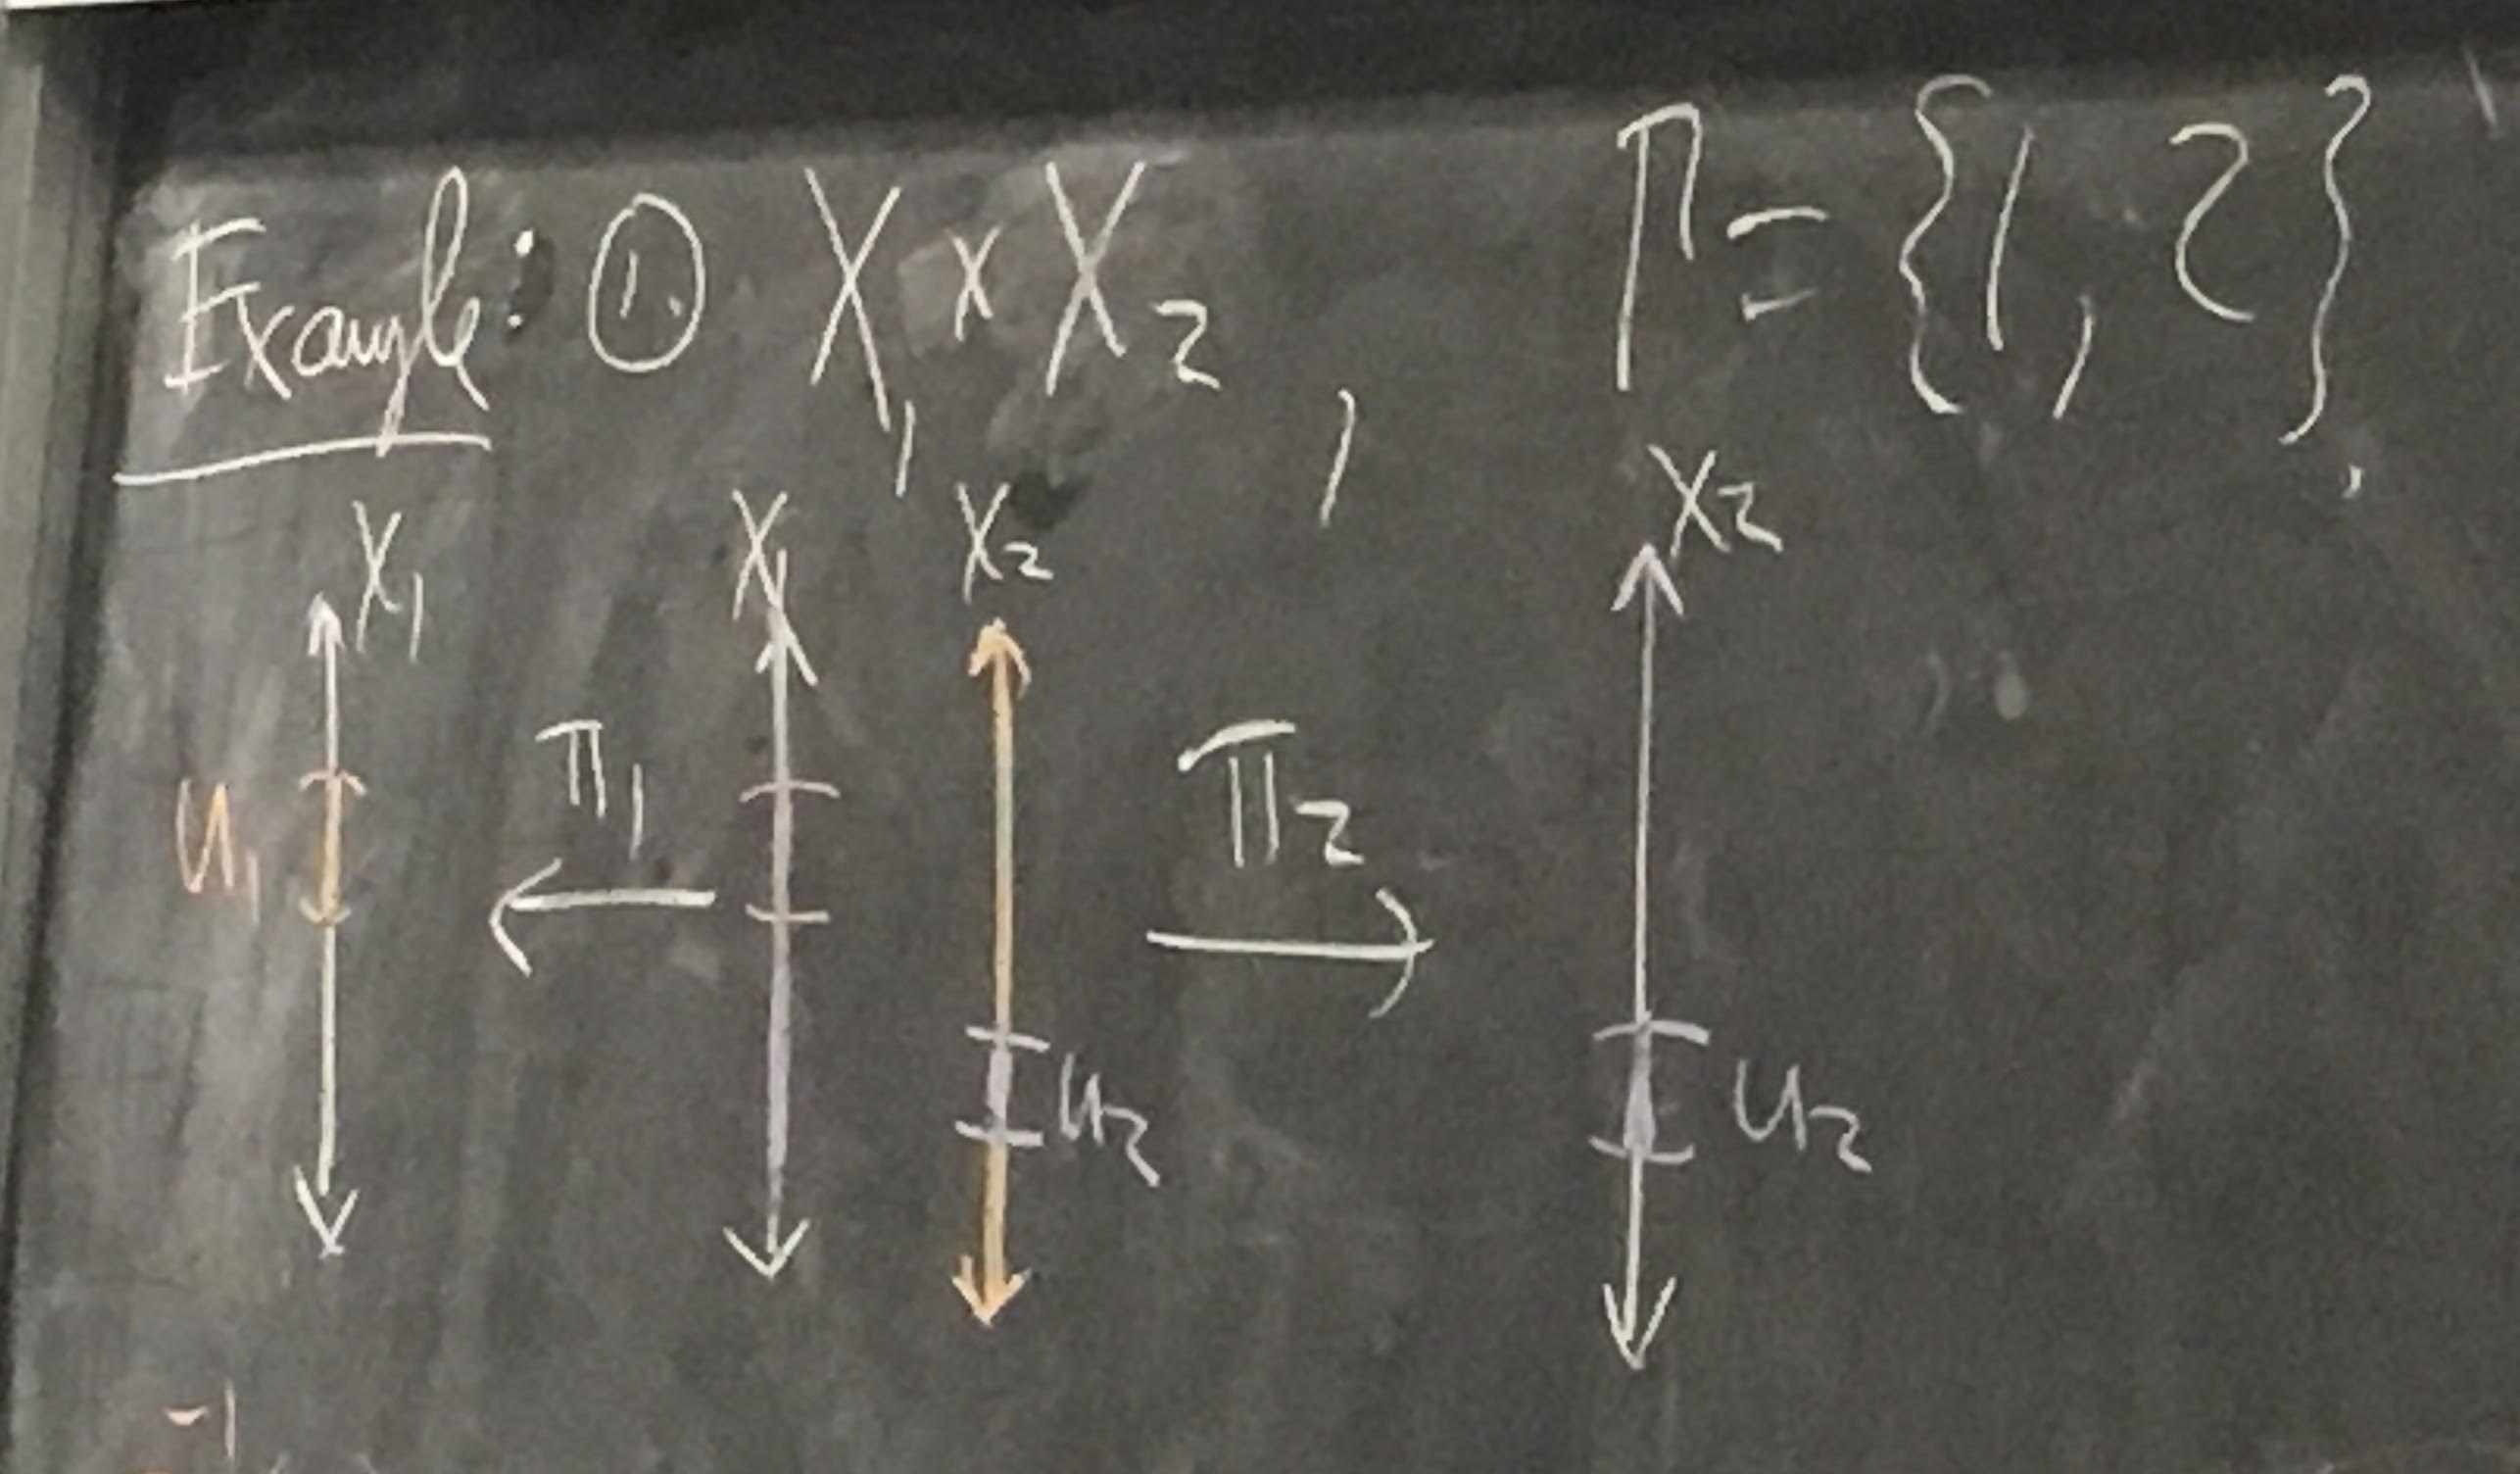
\includegraphics[scale=.08]{images/general_products1}
\end{center}

\end{example*}

\begin{example*}[2]
Consider $\prod_{i\in\N}R^1_i$

This is countable, so we could legitimately write a sequence of real number to represent vectors in this topology. 

Here's what a set from the subbasis looks like:
\[\prod_{i\in N} U_i,\text{ where }U_i=
\begin{cases}
\R^1 & i\neq j\\
U_j & i=j
\end{cases}
\]

So, the product topology on $\prod_{i\in\N}R^1_i$ has as a basis, sets of the form 
\[\prod_{i\in N} U_i,\text{ where }U_i=
\begin{cases}
\R^1 & i\neq j_1, \ldots, j_N\\
U_j & i = j_1, \ldots, j_N
\end{cases}
\]

So, for instance  
$$(0,1) \times \R \times \R \times  (e,\pi) \times \R \ldots \text{ is open, }$$
but 
$$(0,1) \times (0,1) \times (0,1) \times \ldots \text{ is \emph{not} open, }$$

\end{example*}

\begin{example*}[HW 4.5]
Recall that $\{0,1\}^X := \{f:X\to \{0,1\}\}$. \\

The problem asks to show that given $x\in X$, and $\epsilon=0,1$, and $U(x,\epsilon) = \{f:f(x)=\epsilon\}$; we have that the collection of all $U(x,\epsilon)$ forms a subbasis for a topology on $\{0,1\}^X$. 

(image)

Note that $\{0,1\}^X = \prod_{x\in X}\{0,1\}_x$. Note also that $U(x,\epsilon)=\preimage{\pi_x}{\{\epsilon\}}$. So, the topology in HW 4.5 was actually the product topology on $\prod_{x\in X}\{0,1\}_x$, where each $\{0,1\}_x$ has the discrete topology. 
\end{example*}

\begin{highlight}
\begin{theorem}
Let $\arbcoll{X}$ be a collection of spaces, and let $\arbprod{X}$ have the product topology. Then, for any $\beta\in\Gamma$, $\quad \pi_\beta :\arbprod{X} \to X_\beta$ is continuous, onto, and open. 
\end{theorem}
\end{highlight}
\begin{proof}\mbox{}
\begin{itemize}
\item Let $U_\beta$ be open in $X_\beta$. Then, $\preimage{\pi_\beta}{U_\beta}$ is open in $\arbprod{X}$ by definition. 
\item To see that projections are onto, let $x_\beta\in X_\beta$. Then for any $f\in\arbprod{X}$ with $f(\beta)=x_\beta$, then $\pi_\beta(f)=f(\beta)=x_\beta$. 
\item To see that $\pi_\beta$ is open, consider a basic open set $\bigcap\limits_{i=1}^N \preimage{\pi_{\alpha_i}}{U_{\alpha_i}}$, for some $\alpha_1, \ldots \alpha_N \in \Gamma$. Then the image in $\pi_\beta$ is as follows: 
\[\pi_\beta\left(\bigcap\limits_{i=1}^N \preimage{\pi_{\alpha_i}}{U_{\alpha_i}}\right)=
\begin{cases}
X_\beta & \beta\neq\alpha_1, \ldots \alpha_N\\
U_\beta & \beta=\alpha_1, \ldots \alpha_N\\
\end{cases}\]
which is a basic open set in the product topology. 
\end{itemize}
\end{proof}

\begin{highlight}
\begin{theorem}
Let $\arbcoll{X}$ be a collection of Hausdorff spaces. Then, $\arbprod{X}$ is Hausdorff (with respect to the product topology). 
\end{theorem}
\end{highlight}
\begin{proof}
Let $f\neq g\in \arbprod{X}$. In particular, there exists some $\alpha_0$ where $f(\alpha_0)\neq g(\alpha_0)$. 

\begin{center}
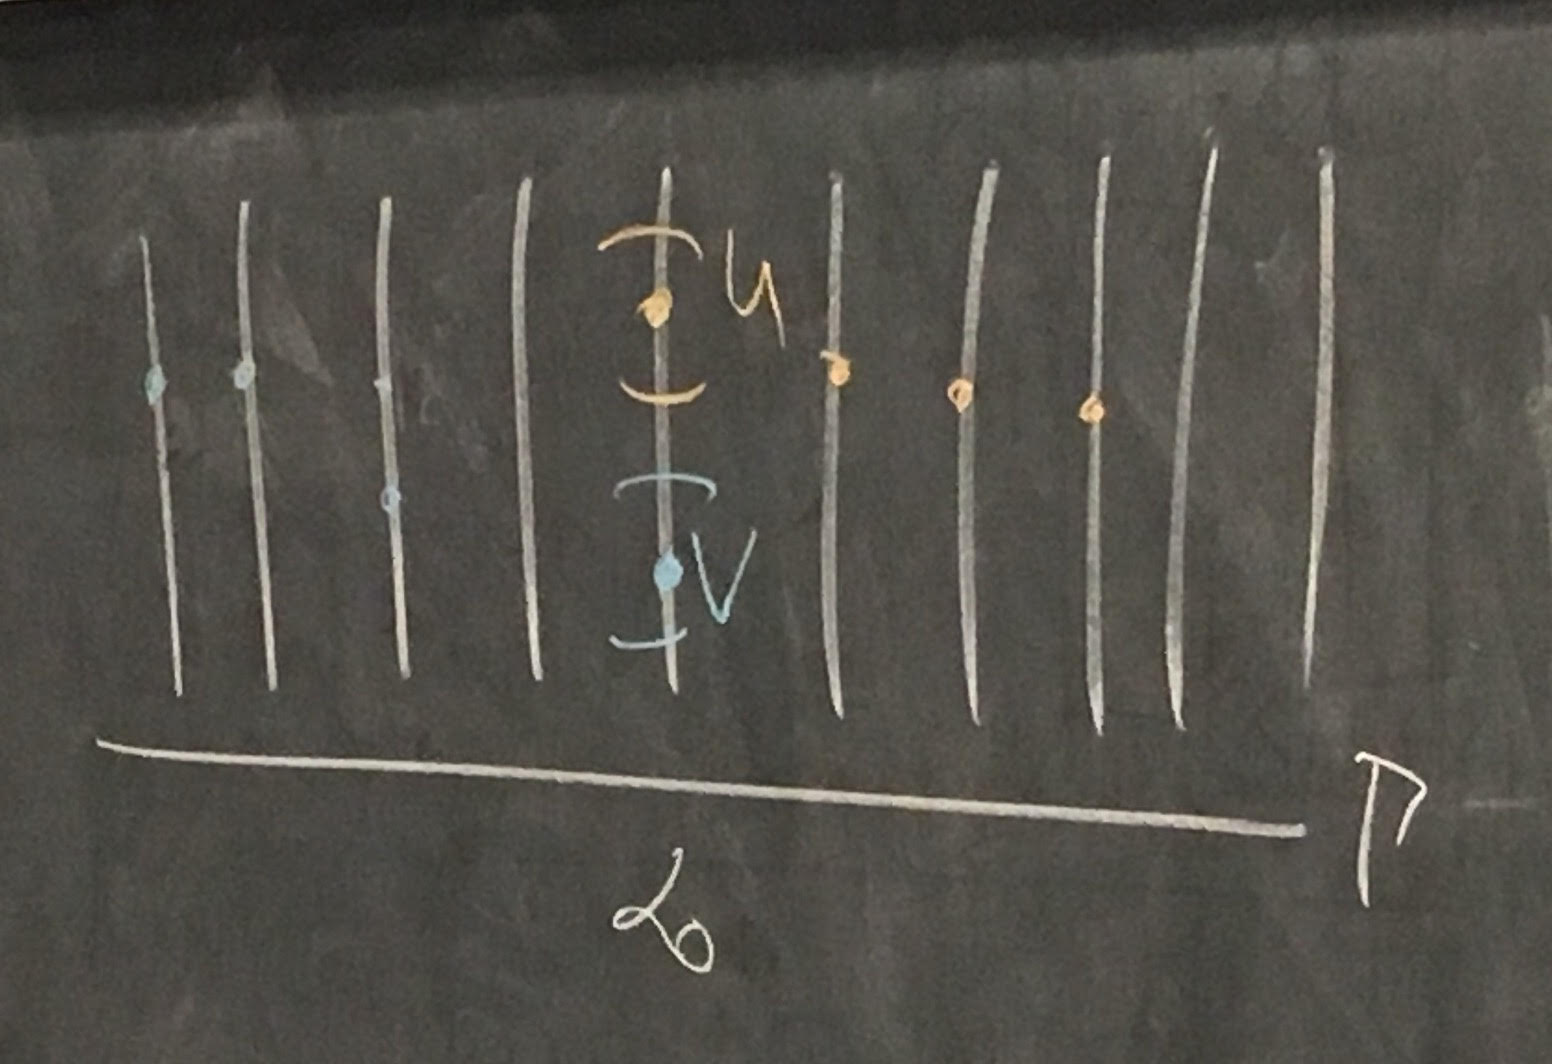
\includegraphics[scale=.12]{images/general_products2}
\end{center}

Since $X_0$ is Hausdorff, there exist open sets $U,V \in X_{\alpha_0}$ with $f(\alpha_0)\in U, g(\alpha_0)\in V$, and $U\cap V=\emptyset$. But then we have $f\in \preimage{\pi_{\alpha_0}}{U}$, and $g\in \preimage{\pi_{\alpha_0}}{V}$, and $\preimage{\pi_{\alpha_0}}{U} \cap \preimage{\pi_{\alpha_0}}{V} = \emptyset$. Thus, we have produced two disjoint open sets in the product topology (they are subbasic sets, by the way) which contain $f$ and $g$, respectively. 
\end{proof}

\begin{highlight}
\begin{definition*}
Let $\arbcoll{X}$ be a collection of scpaces. The collection of all sets $\arbprod{X}$ with $U_\alpha$ open in $X_\alpha$ for all $\alpha\in\Gamma$ is a basis for a topology on $\arbprod{X}$, called the \emph{box topology}. 
\end{definition*}
\end{highlight}

\begin{example*}[1]
If $\Gamma=\{1,\ldots, n\}$, there is no difference between the box topology on $\prod\limits_{i=1}^n X_i $ and the product topology. 
\end{example*}

\begin{example*}[2]
Consider $\prod\limits_{i\in\N}\R^1_i$ where each $\R^1_i$ has the usual topology. We saw already that $\prod\limits_{i\in\N}(0,1)$ is not open in the product topology, but $\prod\limits_{i\in\N}(0,1)$ \emph{is} open in the box topology. 
\end{example*}

\begin{highlight}
\begin{theorem}[Alexander Subbasis Theorem]
Suppose $X$ is a space given by a subbasis $\script{S}$. If every open cover of $X$ by sets in $\script{S}$ has a finite subcover, then $X$ is compact. 
\end{theorem}
\end{highlight}
\begin{proof}
To prove this, you need some axioms from set theory, so we won't prove it in this class. For more information, google these:
\begin{itemize}
\item Zorn's Lemma
\item The Axiom of Choice
\item Well-ordering Principle (this might not mean what you think it means)
\end{itemize}
By the way, it can be proved that these three axioms are equivalent. 
\end{proof}
\begin{highlight}
\begin{theorem}[Tychonoff Theorem]
$\arbcoll{X}$ compact, if and only if $\arbprod{X}$ with the product topology is compact. 

This does \emph{not} hold with the box topology. 
\end{theorem}
\end{highlight}
\begin{proof}$(\implies)$ (Using Alexander Subbasis Thm).
Suppose $\arbprod{X}$ is not compact, but each $X_\alpha$ is compact. By the Alexander Subbasis Theorem, there exists a subbasic open cover $\script{S}_0$ of $\arbprod{X}$ with no finite subcover. For each $\alpha\in\Gamma$, consider 
$$\script{C}_\alpha=\{U \text{ open in }X_\alpha: \preimage{\pi_\alpha}{U}\in\script{S}_0\}.$$
Note that for any $\alpha$, $\script{C}_\alpha$ cannot be an open cover of $X_\alpha$ (because if it were, we would have a finite subcover $\finitecoll{U}$, and then the collection $\finitefuncts{\inv{\pi_\alpha}}{U}$ would be an open cover by sets in $\script{S}_0$ of $\arbprod{X}$).
This mean for any $\alpha$, there is $x_\alpha\in X_\alpha$ with $x_\alpha\not\in\script{C}_\alpha$. 
Thus we can define a function $f:\Gamma\to \bigcup\limits_{\alpha\in\Gamma}X_\alpha$ by $f(\alpha)=x_\alpha\in X_\alpha$ (as constructed). We can then consider $f$ to be a point in $\arbprod{X}$, but $f$ is not contained in any member of $\script{S}_0$. This means that $\script{S}_0$ cannot cover $\arbprod{X}$, which contradicts our assumption. 
\end{proof}

\begin{highlight}
\begin{theorem}
Let $\arbcoll{X}$ be a collection of connected spaces. Then, $\arbprod{X}$ is connected (with respect to the product topology). 
\end{theorem}
\end{highlight}
\begin{proof}
Let $f\in\arbprod{X}$. For any $\alpha_0\in\Gamma$, let 
\[\script{C}_{\alpha_0}=\prod_{\alpha\in\Gamma}
\begin{cases}
X_{\alpha_0} &  \alpha=\alpha_0\\
\{f(\alpha)\} &   \alpha\neq\alpha_0\\
\end{cases}\]
%Let $f\in\arbprod{X}$. For any $\alpha_0\in\Gamma$, let $\script{C}_{\alpha_0}=\prod\limits_{\alpha\in\Gamma} D_\alpha$, where 
%\[D_{\alpha}=
%\begin{cases}
%X_{\alpha_0} &  \alpha=\alpha_0\\
%\{f(\alpha)\} &   \alpha\neq\alpha_0\\
%\end{cases}\]
\begin{center}
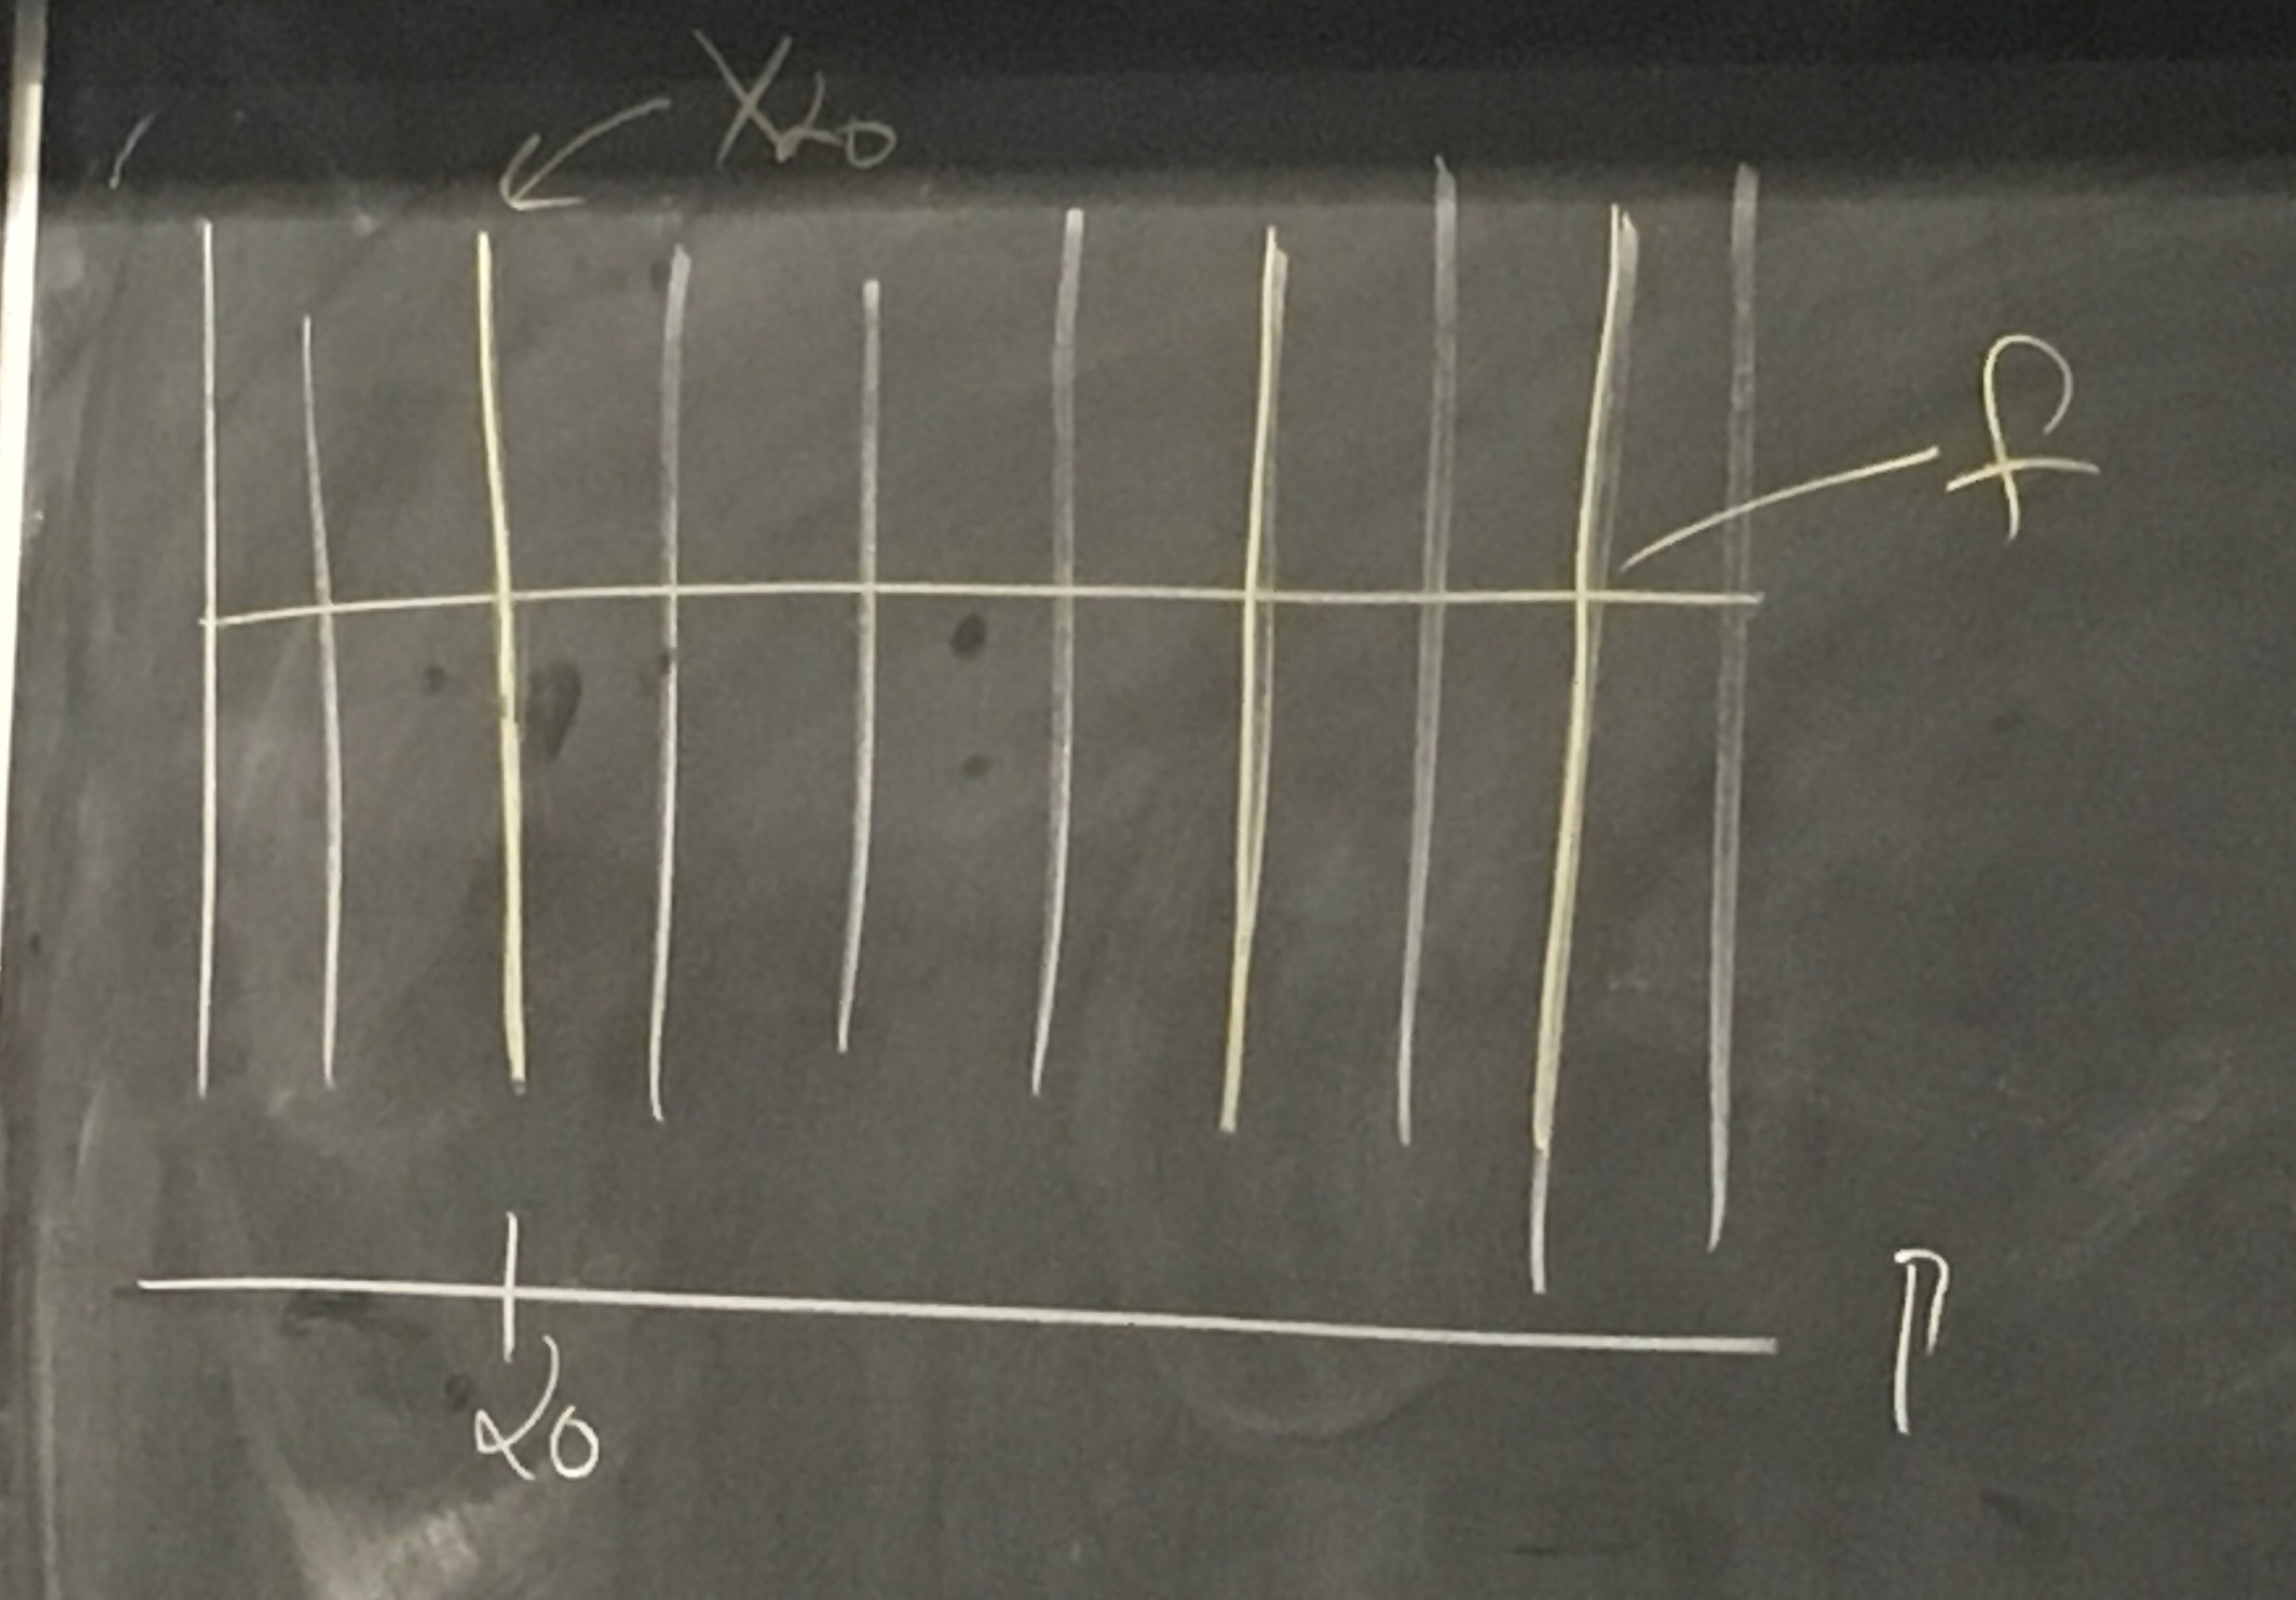
\includegraphics[scale=.08]{images/thm54_1}
\end{center}
We can show that $\script{C}_{\alpha_0} \cong X_{\alpha_0}$. For any finite collection $\beta_1, \ldots, \beta_n \in \Gamma$, we have that $\script{C}_{\beta_1} \cup \ldots \cup \script{C}_{\beta_n}$ is connected by Theorem 45.
Also, 
$$C = \bigcup_{\{\beta_1, \ldots, \beta_n\}\text{ is a finite subset of }\Gamma} \script{C}_{\beta_1} \cup \ldots \cup \script{C}_{\beta_n}$$
is connected, also by Thm 45. 

\noindent \textbf{Claim:} $\closure{C}=\arbprod{X}$. Note that if true, this suffices to prove the theorem.
\begin{proof}[\textbf{Proof of Claim}]\let\qed\relax
Let $g\in\arbprod{X}$, and let $U$ be a basic open set with $g\in U$. By definition, $U=\arbprod{U}$ with $U_\alpha = X_\alpha$ except for finitely-many component sets. 

\begin{center}
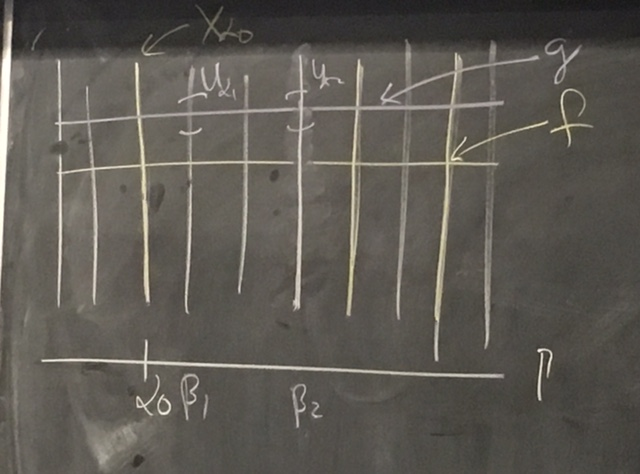
\includegraphics[scale=.3]{images/thm54_2}
\end{center}

But then $U\cap(\script{C}_{\beta_1} \cup \ldots \cup \script{C}_{\beta_n})\neq\emptyset$ because it contains 
\[h(\alpha)=
\begin{cases}
g(\alpha) & \alpha=\beta_1, \ldots, \beta_n \in \Gamma\\
f(\alpha) & \alpha\neq\beta_1, \ldots, \beta_n \in \Gamma\\
\end{cases}\]
\end{proof}
\end{proof}


\end{document}